\documentclass[11pt,a4paper]{article}
%\textheight = 630pt
%\textwidth = 480pt
%\topmargin = 3pt
%\voffset = 0pt
%\headsep = 2pt
%\headheight = 1pt
%\oddsidemargin = 1pt
%\marginparwidth = 1pt
%%%%%%%%%%%%%%%%%%%%%%%%%%%%%%%%%%%%%%%%%%%%%%%%%%%%
%TODO Use this website for formatting http://codeinthehole.com/writing/writing-a-thesis-in-latex/
%%%%%%%%%%%%%%%%%%%%%%%%%%%%%%%%%%%%%%%%%%%%%%%%%%%%
%% Save space packages and settings %%
\usepackage{cite}

%\usepackage{paralist}
%\usepackage[compact]{titlesec}
%\titlespacing{\section}{0pt}{0.5ex}{0.5ex}
%\titlespacing{\subsection}{0pt}{0.5ex}{0ex}
%\titlespacing{\subsubseSction}{0pt}{0.5ex}{0ex}
%\linespread{1}

\usepackage[left=1.5in, right=1in, top=1in, bottom=1in, includefoot, headheight=13.6pt]{geometry}

\usepackage{bm}
\usepackage{changepage}
%\usepackage[hmargin=2.5cm, vmargin=4cm]{geometry}
\usepackage{parskip}
\setlength{\parskip}{5pt}
\usepackage{fancyvrb}
\usepackage{graphicx}
\usepackage{amsmath}
\usepackage{capt-of}
\usepackage{amsfonts}
\usepackage{verbatim}
\usepackage{courier}
\usepackage{float}
\restylefloat{table}
\usepackage[english]{babel}
\usepackage{algorithm2e}
\usepackage{soul}
\usepackage{hyperref}


%%%%%%%%%%%%%%%%%%%%%%%%%%%%%%%%%%%%%%%%%%
%% Commands
\newcommand{\inreal}{\in \mathbb{R}}
\newcommand{\inrealmxn}{\in \mathbb{R}^{m\times n}}
\newcommand{\inintmxn}{\in \mathbb{Z}^{m\times n}}
\newcommand{\inints}{\in \mathbb{Z}}
\newcommand{\innatural}{\in \mathbb{N}}
\newcommand{\smat}{\mathbf{S}}
\newcommand{\covmat}{\mathbf{A}}
\newcommand{\xvec}{\mathbf{x}}
\newcommand{\vvec}{\mathbf{v}}
\newcommand{\vmat}{\mathbf{V}}
\newcommand{\tp}{^T}
\DeclareMathOperator{\Tr}{Tr}
\newcommand{\new}{_\text{new}}
\newcommand{\old}{_\text{old}}
\newcommand{\common}{_\text{common}}



%%%%%%%%%%%%%%%%%%%%%%%%%%%%%%%%%%%%%%%%%%
\begin{document}

\begin{titlepage}

\newcommand{\HRule}{\rule{\linewidth}{0.5mm}} % Defines a new command for the horizontal lines, change thickness here

\center % Center everything on the page
 
%----------------------------------------------------------------------------------------
%	HEADING SECTIONS
%----------------------------------------------------------------------------------------

\textsc{\LARGE Imperial College London}\\[1.5cm] % Name of your university/college
\textsc{\Large Department of Electrical \& Electronic Engineering}\\[0.5cm] % Major heading such as course name
\textsc{\large MEng Project Report}\\[0.5cm] % Minor heading such as course title

%----------------------------------------------------------------------------------------
%	TITLE SECTION
%----------------------------------------------------------------------------------------

\HRule \\[0.4cm]
{ \huge \bfseries Analysing Twitter Data Using Sparse PCA}\\[0.4cm] % Title of your document
\HRule \\[1.5cm]
 
%----------------------------------------------------------------------------------------
%	AUTHOR SECTION
%----------------------------------------------------------------------------------------

\begin{minipage}{0.4\textwidth}
\begin{flushleft} \large
\emph{Author:}\\
 \textsc{Theo Pavlakou} % Your name
\end{flushleft}
\end{minipage}
~
\begin{minipage}{0.4\textwidth}
\begin{flushright} \large
\emph{Supervisor:} \\
\textsc{Dr. Moez Draief} % Supervisor's Name
\end{flushright}
\end{minipage}\\[4cm]

% If you don't want a supervisor, uncomment the two lines below and remove the section above
%\Large \emph{Author:}\\
%John \textsc{Smith}\\[3cm] % Your name

%----------------------------------------------------------------------------------------
%	DATE SECTION
%----------------------------------------------------------------------------------------

{\large \today}\\[3cm] % Date, change the \today to a set date if you want to be precise

\vfill % Fill the rest of the page with whitespace

\end{titlepage}

\pagenumbering{gobble}




\newpage




\section*{\center Abstract}
\begin{comment}
- Inspired by the work of Dimakis and Microblogs, seek to combine the work.
- Evaluate Sparse PCA algorithms for the general case and for the specific binary matrix case. 
- Altered the input matrix to improve results. 
- Tests are done on Twitter data and results confirmed by real life events.
- A streaming app created with automatic event recognition. 
- Proof of concept. 
- Room for further work.
\end{comment}
With the explosive growth of social media users and the ease by which one can retrieve user data, there has recently been a plethora of research being done focusing on how this data can be used to make useful inferences and find trends in populations. The purpose of this study is to develop the framework for an application that can be used to automatically detect events from Twitter data in an online fashion, using a class of techniques collectively referred to as Sparse Principal Component Analysis (SPCA). These are similar to regular Principal Component Analysis, however, they produce vectors which do not have many non-zero entries, which helps with their interpretation in areas such as document analysis. Methods to improve the output of SPCA for the specific context are presented by altering the input co-occurrence matrix and one variant is shown to consistently outperform the rest. Added to this, various SPCA algorithms are evaluated against one another, bearing in mind the specific needs of the final application. A streaming application is then developed and its performance is tested using real Twitter data by confirming that the results obtained align well with events that happened within the time period being considered. 

\clearpage
\section*{\center Acknowledgments}
The work presented in this project would not be possible without the help and support of many people. 

Firstly, I would like to thank my supervisor, Dr. M. Draief, who has been there to advise and encourage me throughout the whole process. I would also like to thank Dr. A. Babaee, who has given me insights into the standard practices of research and has helped me with finding data so that the necessary measurements could be made and the mathematical concepts presented could be validated. 

My fiancee, my family, my friends and my community have also been understanding and supportive the whole way and their love and care has been a great comfort throughout.
\clearpage
\tableofcontents
\newpage
%\clearpage
\pagenumbering{arabic}

\section{Introduction}
Social media now shapes our lives in such a vast way. More than $98\%$ of 18-24 year olds use social media, such as Facebook, Twitter and Instagram, and most use them more than half an hour a day on average.\footnote{http://www.statisticbrain.com/social-networking-statistics, Accessed: 21-12-2013.} Recently there has been a lot of work that has gone into analysing this vast amount of data that is available freely on the internet to understand trends in populations and to be able to target particular groups for marketing purposes. The term ``Big Data'' has become very widely used and the data that we encounter in these social media fit straight into this category. Machine learning algorithms and mathematical techniques can be used on this noisy data to infer useful results that can further be used to predict future trends. 

One such technique is known as Principal Component Analysis (PCA) and is concerned with finding linear combinations of the variables in a set of features which lead to the highest variation in outcomes, which in turn means leading to the highest information gain. The problem with PCA is that it can be hard to interpret since the size of the vector that is returned could be immense in length, e.g. 3000 entries, with only a few entries being of significance. This has led to the creation of algorithms that return sparse representations approximating the principal components, but which lead to results that are much easier to interpret. In this project the algorithms currently present to perform sparse PCA are analysed and evaluated using primarily a batch of Twitter data gathered from London in 2012 \footnote{This data has been provided by the authors of \cite{microblogs}.}. Then methods of improvement to the algorithms is also considered by cleaning the data before using it as input to the algorithm. An application is then created which can be used to automatically detect events from a stream of Tweets, by using the Sparse PCA algorithm chosen, and methods to improve the final application are explored. 
%TODO possibly put organisation here. 

%% Mention only if reference is found
%Lots of money goes into this yearly, and companies such as Google and Facebook spend \textbf{(Find number and cite)} per year on such methods to maintain their competitive edge in industry. 

\begin{comment}
\section{Project Specification}
%TODO Change this title or merge with previous section

The purpose of this study is to examine how a certain implementations of Sparse PCA can help to infer results from data, focusing on that of social media which can be represented as a binary matrix. The performance of various algorithms are to be compared and evaluated against one another, with a special focus on the algorithm in \cite{dimakis} as this project can be seen as a continuation of their work. The data used is a batch of Tweets from London throughout the year 2012. The reason Twitter data has been chosen is due to the character limit imposed on each Tweet, which means that each message is typically quite information dense, which is best to test the algorithm and come up with useful results in the first iteration. Later improvements may be used on lengthier texts, but a more sophisticated parser may need to be used in that scenario. After concluding meaningful results from the data as a whole, windowing the data into smaller periods of time is also attempted and an evolution of the results is examined further to see how the principal components correlate to events that happened in 2012. Measures to improve the performance and the scalability of the resulting algorithm are also explored and further improvements are researched.

\end{comment}
\section{Notation}

Throughout the remaining sections, the following mathematical notations will be used. $\mathbf{S} \in \mathbb{Z^*}^{m\times n}$ is the data matrix consisting of $m$ data points (in the specific case considered in depth in this paper, the Tweets) evaluated on $n$ features (words), with $[\mathbf{S}]_{i,j} = 1$ when Tweet $i$ contains word $j$ and zero otherwise. Likewise, the variable $m$ is reserved for the number of Tweets and $n$ for the number of words. $\mathbf{A} \in \mathbb{Z^*}^{n \times n}$ is equal to $\mathbf{S}^T\mathbf{S}$ or a variant of this and it corresponds to the co-occurrence matrix of $\mathbf{S}$. $\mathbf{v}_i$ is to be used for the eigenvector with the $i$th largest eigenvalue, correspondingly denoted by $\lambda_i$. Both $\|\mathbf{x}\|$ and $\|\mathbf{x}\|_2$ denote the $l_2$ norm of a vector, defined as $\sqrt{\mathbf{x}^T\mathbf{x}}$ and $\|\mathbf{x}\|_0$ denotes the $l_0$ norm of a vector, defined as the number of non-zero elements in it. $[\mathbf{x} ]_i$ denotes the $i$th element in a vector and similarly $[\mathbf{A}]_{i, j}$ denotes the element specified by the $i$th row and the $j$th column. For a matrix, $\|\mathbf{A}\|_F$ defines the Frobenius norm, defined as $\sqrt{\sum^m_{i=1}{\sum_{j=0}^n{\mathbf{[A}]_{i, j}^2}}}$.

\section{Organisation}
%TODO
\section{Background}
%TODO Add a section that explains microblogs and other event finding algorithms
To understand the project in detail, it is necessary to first understand some of the underlying methods that are used and the theory supporting them. In this section, an attempt is made to give a thorough enough explanation whilst not going too in depth to diverge from the main topic of discussion. It also gives reasons as to why this project is important, what work has already been done in this field and why the particular direction has been chosen. 

%\textbf{Not done:}
%\begin{itemize}
%\item Explain SVD in this scenario and how it relates (see http://people.cs.pitt.edu/~milos/courses/cs3750-Fall2007/lectures/PCA.pdf)?
%\end{itemize}



\subsection{Principal Component Analysis (PCA)}
\subsubsection{Description}
Principal Component Analysis is a method that can be used to reduce the dimensionality of a data set by projecting it onto the principal subspace that is spanned by the eigenvectors with the largest eigenvalues of the covariance matrix. The reason that the largest eigenvalue eigenvectors are chosen is because these are the eigenvectors along which the largest variance occurs and therefore the most information can be retrieved from (see Appendix for a more thorough proof of this). This can be seen in Figure \ref{pca}. Here we have a two dimensional data set, say $\mathbf{S} \in \mathbb{R}^{m \times 2}$, where $m$ is the number of data points, which has been plotted on the first of the three graphs. It can be seen, however, that the points vary from the blue line only slightly, which means that, if the data can be projected onto this direction, the data can be approximated by only one component. When performing principal component analysis, the principal components that are found are:

\begin{equation*}
\mathbf{V} = 
\begin{pmatrix}
\mathbf{v}_1 && \mathbf{v}_2
\end{pmatrix} = 
\begin{pmatrix}
0.6956 && 0.7184\\
 0.7184 && -0.6956\\
\end{pmatrix}.
\end{equation*}

We can then project the data onto the new principal components, as such:

\begin{equation*}
\mathbf{S}_p = \mathbf{S}\mathbf{V},
\end{equation*}
where $\mathbf{S}_p \in \mathbb{R}^{m \times 2}$ is the data projected onto the new principal components, namely $\mathbf{v}_1$ and $\mathbf{u}_2$. The plot of this new data can be seen in the second graph. 

In the third graph we project the data only onto $\mathbf{v}_1$ i.e.
\begin{equation*}
\mathbf{S}_p = \mathbf{S}\mathbf{v}_1.
\end{equation*}

As it can be seen, this graph only differs by the second graph by a small amount but only half the features have been used. This is an example of dimensionality reduction (or compression). In this case, the number of features has been reduced to half the number before, but a lot more than half the variation has been maintained. In the application of PCA explored here, the second stage is more important, as the variation direction is what is considered most and not the compression, but this has been added for completeness.

The first principal component (i.e. the first eigenvector of the $n\times n$ matrix, $\mathbf{A}$) is:
\begin{equation}
\mathbf{v}_1 = \underset{\|\mathbf{x}\|^2 = 1}{\operatorname{argmax}}\left( \mathbf{x}^T\mathbf{A}\mathbf{x}\right).
\end{equation}
Here $\covmat$ is the covariance matrix associated with the data points. Principal Component Analysis alongside Singular Value Decomposition is explained further in \cite{datascience} and \cite{bishop}. 

\begin{figure}[H]
\centering
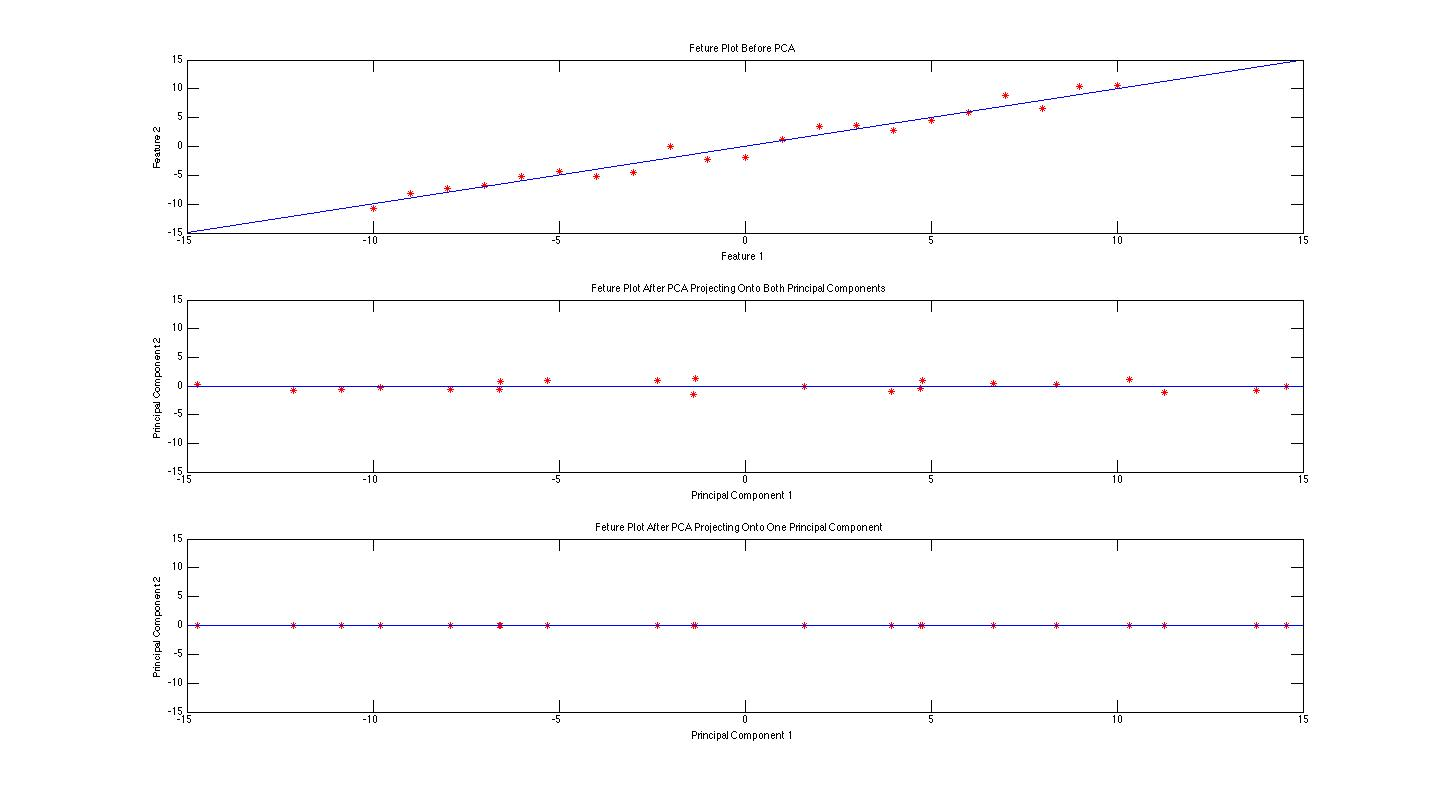
\includegraphics[scale=0.35]{PCA_EXPLAINED.jpg}
\caption{Graphs demonstrating what PCA does. The first graph shows the plot of the features before performing the PCA. The second shows the features projected onto both the new principal components and the third shows the data points only projected onto the first principal component.}
\label{pca}
\end{figure}

\subsection{Similarity to Singular Value Decomposition (SVD)}
This work is largely an extension of \cite{lecture_svd}.

\subsubsection{Description}
SVD is a decomposition method that is very important in many areas due to the way it factorises a matrix into 3 matrices, each with a very informative structure. The basic decomposition is as such:
\begin{equation}
\mathbf{S} = \mathbf{U}\mathbf{\Sigma}\mathbf{V}^T,
\end{equation}
where $\mathbf{S} \in \mathbb{R}^{m \times n}$,  $\mathbf{U} \in \mathbb{R}^{m \times r}$ and is a column orthonormal matrix, where $r$ is equal to the rank of the matrix,  $\mathbf{V} \in \mathbb{R}^{n \times r}$ is also a column orthonormal matrix, and  $\mathbf{\Sigma} \in \mathbb{R}^{r \times r}$ is a diagonal matrix where the elements are sorted in descending order.

\subsubsection{Example Related to Project}
In the scenario considered in this paper, the matrix $\mathbf{S}$ is a matrix with the rows representing the tweets and the columns representing the words (features). The matrix is made up of only ones and zeros, with $[\mathbf{S}]_{i,j} = 1$, if tweet $i$ contains word $j$ and zero otherwise. As a toy example, let:
\begin{equation}
\mathbf{S} = 
\begin{pmatrix}
1 & 1 & 1 & 0 & 0\\
1 & 1 & 1 & 0 & 0\\
1 & 1 & 1 & 0 & 0\\
0 & 0 & 0 & 1 & 1\\
0 & 0 & 0 & 1 & 1\\
0 & 0 & 0 & 1 & 1\\
0 & 0 & 0 & 1 & 1\\
\end{pmatrix}
\end{equation}
Where the columns represent the ordered bag of words, referenced from left to right \{football, cup, win, cyprus, eu\}, and there are two main topics trending on Twitter. One is about some football victory, and the other is about Cyprus joining the EU. This is a very artificial example as it assumes that the Tweets would contain the exact same words, but a more general example will be given later. As it can be seen, this matrix is of rank 2, which is also the number of topics that are presented by the matrix. 

Performing the SVD on the matrix, what is acquired is:

\begin{equation*}
\mathbf{S} = \mathbf{U}\mathbf{\Sigma}\mathbf{V}^T
\end{equation*}

\begin{equation}
\mathbf{S} = \begin{pmatrix}
-0.5774 & 0.0000\\
-0.5774 & 0.0000\\
-0.5774 & 0.0000\\
0.0000 & -0.5000\\
0.0000 & -0.5000\\
0.0000 & -0.5000\\
0.0000 & -0.5000\\
\end{pmatrix}
\begin{pmatrix}
3.0000 & 0.0000\\
0.0000 & 2.8284\\
\end{pmatrix}
\begin{pmatrix}
-0.5774 & -0.5774 & -0.5774 & 0.0000 & 0.0000 \\
0.0000 & 0.0000 & 0.0000 & -0.7071 & -0.7071\\
\end{pmatrix}.
\end{equation}

These three matrices all have a very significant meaning. It has already been stated that due to the obvious form of $\mathbf{S}$ it can be seen that there are only 2 topics or concepts. The $\mathbf{U}$ matrix can be viewed as the Tweet to concept correlation matrix i.e. how correlated the Tweets are to the corresponding topics. Similarly, the $\mathbf{V}^T$ matrix can be viewed  the concept to word correlation matrix i.e. how related the concept is to the particular word. For example, $\mathbf{U}_{2,1}$ would be how related the second Tweet is to the first concept and $\mathbf{V}^T_{2,3}$ would be how related the second topic is related to the third word, which in this case is zero, i.e. there is no similarity, because the second concept is about Cyprus joining the EU and the third word is win, which does not appear in any Tweet regarding Cyprus and the EU. The $\mathbf{\Sigma}$ matrix is then just the concept strengths.

It can then be shown that $\mathbf{S}^T\mathbf{S}$ represents the correlation of the words in the tweets to each other, i.e. a covariance matrix (see Appendix). But 
\begin{align*}
\mathbf{S}^T\mathbf{S} &= \mathbf{V}\mathbf{\Sigma}\mathbf{U}^T \mathbf{U}\mathbf{\Sigma}\mathbf{V}^T,\\
& = \mathbf{V}\mathbf{\Sigma}^2\mathbf{V}^T,\\
& = \mathbf{V}\mathbf{\Lambda}\mathbf{V}^T,
\end{align*}
which essentially means that the columns of $\mathbf{V}$ are the eigenvectors of the matrix $\mathbf{S}^T\mathbf{S}$ and the diagonal values of $\mathbf{\Lambda}$ are the corresponding eigenvalues, which are the squares of the singular values found in $\mathbf{\Sigma}$.

As it can be seen, there is a close relationship between SVD and PCA, which uses the eigenvectors of the covariance matrix. Therefore, to find the principal components of a matrix $\mathbf{S}$, the SVD can instead be found and the principal components would be the columns of $\mathbf{V}$ (or of $\mathbf{U}$ if we want to find the principal components of $\mathbf{S}\mathbf{S}^T$) and the variances are given by squaring the singular values.

\subsubsection{Further Example Related to Project}
Suppose the matrix $\mathbf{S}$ instead looked like this:

\begin{equation}
\mathbf{S} = 
\begin{pmatrix}
1 & 1 & 1 & 0 & 0\\
1 & 1 & 1 & 0 & 0\\
1 & 1 & 1 & 0 & 0\\
0 & 0 & 0 & 1 & 1\\
0 & 0 & 0 & 1 & 1\\
0 & 0 & 0 & 1 & 1\\
0 & 0 & 0 & 1 & 1\\
1 & 0 & 0 & 1 & 0\\
1 & 1 & 1 & 0 & 0\\
0 & 0 & 0 & 1 & 1\\
0 & 0 & 0 & 1 & 1\\
0 & 0 & 0 & 1 & 1\\
1 & 0 & 0 & 1 & 1\\
\end{pmatrix},
\end{equation}
with the same words representing the columns as in the previous example. It can be seen here that there are now 4 linearly independent columns and therefore this matrix is of rank 4. 

The SVD then turns out to give:


\begin{equation*}
\mathbf{U}=
\begin{pmatrix}
-0.1216&0.4704&-0.1158&0.0223\\
-0.1216&0.4704&-0.1158&0.0223\\
-0.1216&0.4704&-0.1158&0.0223\\
-0.3241&-0.1199&-0.1320&0.0778\\
-0.3241&-0.1199&-0.1320&0.0778\\
-0.3241&-0.1199&-0.1320&0.0778\\
-0.3241&-0.1199&-0.1320&0.0778\\
-0.2336&0.1097&0.7963&0.5471\\
-0.1216&0.4704&-0.1158&0.0223\\
-0.3241&-0.1199&-0.1320&0.0778\\
-0.3241&-0.1199&-0.1320&0.0778\\
-0.3241&-0.1199&-0.1320&0.0778\\
-0.3888&0.0453&0.4363&-0.8102\\
\end{pmatrix},
\end{equation*}
\begin{equation*}
\mathbf{\Sigma}=
\begin{pmatrix}
4.1377&0.0000&0.0000&0.0000\\
0.0000&3.5113&0.0000&0.0000\\
0.0000&0.0000&1.1637&0.0000\\
0.0000&0.0000&0.0000&0.4426\\
\end{pmatrix},
\end{equation*}
\begin{equation*}
\mathbf{V}=
\begin{pmatrix}
-0.2679&0.5801&0.6613&-0.3930\\
-0.1175&0.5359&-0.3980&0.2014\\
-0.1175&0.5359&-0.3980&0.2014\\
-0.6987&-0.1949&0.2654&0.6352\\
-0.6422&-0.2261&-0.4189&-0.6008\\
\end{pmatrix}.
\end{equation*}
As it can be seen here, it is significantly more difficult to actually be able to distinguish which words contribute significantly to each principal component due to the added noise that rows 8 and 13 give rise to. This example highlights how important sparse principal components are since here the data is only $\in \mathbb{R}^{13 \times 5}$ and it is already quite difficult to interpret and in a real life scenario these numbers are typically much larger in magnitude, for example, in the scenario considered in this paper this grows to be in the tens of thousands Tweets and thousands of words.

What is very useful to see, however, is that the singular values do decrease quite rapidly after the second one. These represent the square roots of the eigenvalues of the covariance matrix, so by squaring them the graph in Figure \ref{spectrum} is obtained.

\begin{figure}[H]
\centering
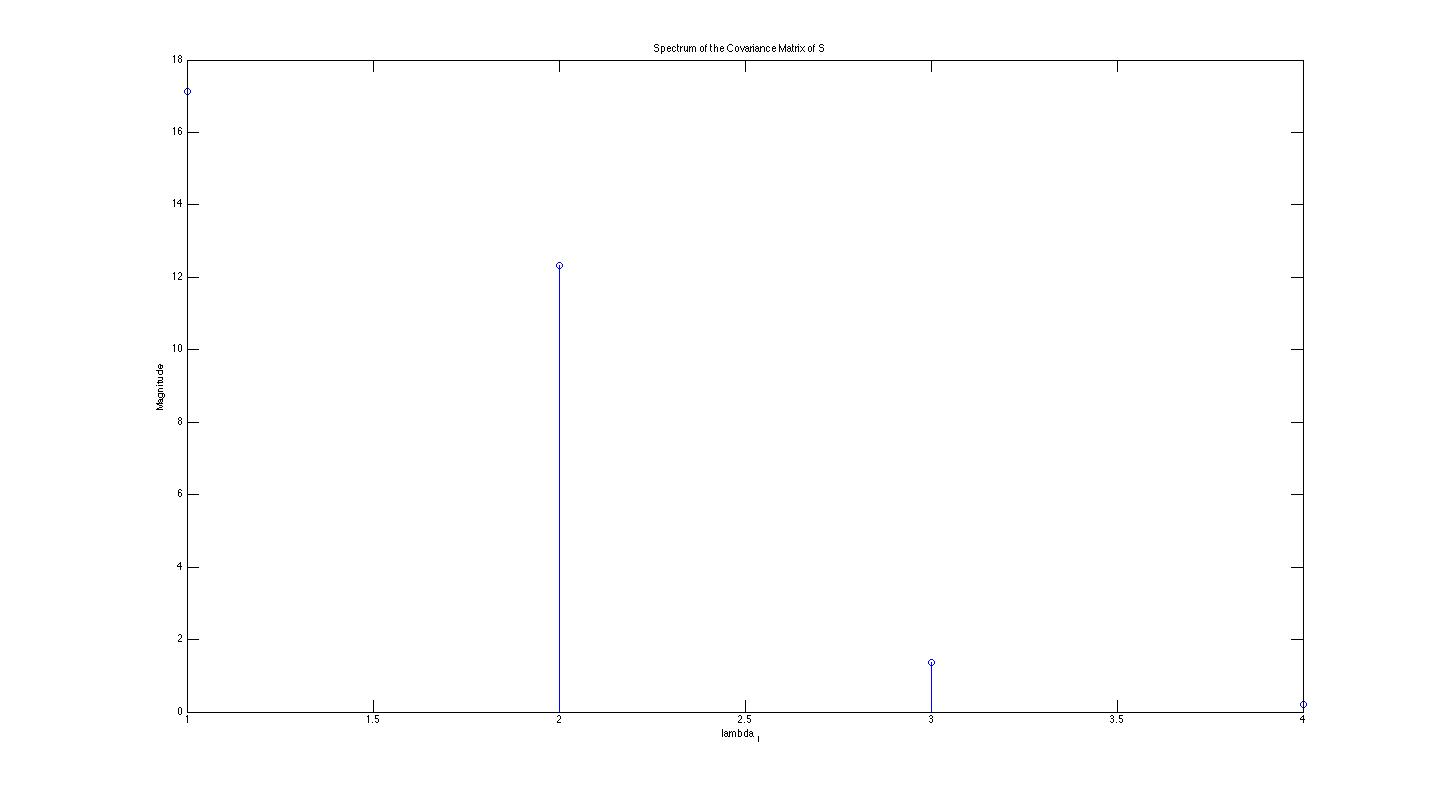
\includegraphics[scale=0.3]{Spectrum_Eigenvalues.jpg}
\caption{The spectrum of the eigenvalues of $\mathbf{S}^T\mathbf{S}$}
\label{spectrum}
\end{figure}

This intuitively makes sense since it is not hard to tell, after looking at the eigenvectors, that the first eigenvector is associated with the words Cyprus and EU, as 7 of the rows only mention these two words from the bag of words. The second eigenvector is associated with the words football, cup and win, as 4 of the rows only contain these words. These are obviously the major concepts and so their eigenvalues are relatively quite high, with the first one being slightly higher. After these however, the eigenvalues fall significantly which relate to the added noise which is present due to the rows 8 and 13, since not much variance can be explained by these two eigenvectors and therefore they carry very little information. 

\subsection{Related Work}
%TODO Must change this as now the focus is quite different
The idea of using social media as a medium for data analysis is not new and much work has been done in this area. Two particular examples are \cite{dimakis} and \cite{microblogs}. These two both lay a solid foundation for the work explored in this paper as it uses a lot of their findings and results and starts where they left off. For instance, the idea of using Sparse PCA to find words that can be associated with events for a particular batch of Tweets has come from \cite{dimakis} and the data used is the same data as was used in \cite{microblogs}. The focus of these, however, is not entirely the same. In \cite{dimakis}, a lot more emphasis is put on the actual algorithm itself, whereas in this paper many other areas are also explored, such as the trade-off between the number of features chosen, the number of points taken and the input to the algorithm itself. Added to this, the final goal of this study is to create a prototype for a streaming application that can be used to automatically find events online, using Sparse PCA as a tool in the process. In \cite{microblogs} the focus is on finding events that match a users query, whereas in this study an attempt is made to find events in an unsupervised manner.

Some of the previous work in both the areas of Sparse PCA and finding events using Twitter will now be presented.

\subsubsection{Sparse PCA}

Sparse PCA algorithms aim to deliver similar results to PCA, but with the difference that they give rise to principal components that only have few non-zero entries. The reason sparsity is desired in the principal components is because sparse approximations of the principal components are useful for interpreting data that have large dimensions. For example, in the specific application discussed in this paper, a set of words is considered and meaningful inferences are to be found from this data. It is clearly much simpler to analyse data given a small set of words that could approximate the variance in the given data set per principal component, than all the words in the data set which would contribute a small amount each, increasing the dimensionality of the principal component to the number of words in the set of all the words in all the Tweets. The equation to be solved resolves to:
\begin{equation}
\mathbf{v}_1 = \underset{\|\mathbf{x}\|_2^2 = 1, \|\mathbf{x}\|_0 = k}{\operatorname{argmax}}\left( \mathbf{x}^T\mathbf{A}\mathbf{x}\right),
\end{equation}
where $\|\mathbf{x}\|_0$ is the $l_0$ cardinality of $x$ i.e. how many non-zero elements x has. This is where Sparse PCA algorithms come in. 

\subsubsection{Methods to perform Sparse PCA}
%TODO Add all the papers to this section.
Plenty of methods have been designed to get sparse principal components or principal component like vectors, due to the importance of such an algorithm in practice, as detailed above. A few are described here, but by no means do these constitute the full work in this active area of research.

The first attempt, and an algorithm that is still widely used regardless of its many limitations is the Thresholding method, which simply performs regular PCA and then forces the entries that are small in magnitude, to zero. This can be misleading and an arbitrary selection of the threshold must be made, which may not actually be valid \cite{cadima}. In \cite{scotlass}, the authors aim to force sparsity by solving the equation
\begin{equation*}
\underset{\substack{\|\mathbf{x}\|_2 = 1, \\ \sum_{j=1}^n|\mathbf{x}| \leq t}}
{\operatorname{argmax}}\mathbf{x}^T\mathbf{A}\mathbf{x},
\end{equation*}
 
for some $t$ where $1<t<\sqrt{n}$, by applying a Lagrange multiplier and then solving a regression type problem. This is done so as to maximise the variance captured by the particular principal component with the constraint that the sum of the entries must be small, which in turn introduces sparsity. This is different to using the $l_2$ norm, which is used in ridge regression and attains variables that are close to, but not exactly, zero and is referred to as the Lasso, which is explained further in \cite{lasso}. Another method which makes use of the Lasso penalty, and various others, can be found in \cite{zou} and \cite{shen}. The method described in \cite{shen} uses the relationship between Singular Value Decomposition (SVD) and PCA as its basis but imposes a penalty on the size of the entries in the principal components. Related to this, and almost identical apart for some pre-processing and post-processing is the Generalised Power Method (GPower) in \cite{GPower}, which is used in this project as a benchmark to compare algorithms. Another attempt has been made by the authors of \cite{daspremont} in which a convex relaxation of the problem is considered to transform it so that it can be solved using Semidefinite Programming. Yet another method is known as the Truncated Power Method (TPower), which can be found in \cite{truncpower} and is also used as a benchmark due to its fast performance. This method performs the well known power method for retrieving the dominant eigenvector of a matrix, but keeps the top $k$ values in magnitude and forces the rest to zero upon each iteration till convergence. 
%TODO Must be changed

\subsubsection{Finding Events using Twitter Data}
%TODO
Finding events in Twitter data can be defined as a particular example of Topic Detection and Tracking (TDT), which was a DARPA-sponsored initiative to investigate how events can be found and tracked in a stream of broadcasts, which the reader can read more about in \cite{tdt}. In this particular case, the broadcasting channel is Twitter. Since then, much work has been done on finding events in a Twitter stream, and other similar work, such as finding the most useful words to describe events in a Twitter stream or event summarisation using Tweets\cite{eventsummary} etc. 
The authors of \cite{petrovic} aim to find events in an unsupervised learning mechanism based on clustering. The basic principle is to represent Tweets as a vector (using the Bag-Of-Words model, described later) and new Tweets are compared to the stored ones using a distance measure. If the distance to all is quite large, it is declared as a new story. Various mechanisms are employed to keep the complexity low also. In \cite{earthquake} a system is created which can detect earthquakes with a high probability based on Tweets and the Twitter user's locations also. Furthermore, an attempt to find events in an online manner using online clustering is done in \cite{Becker_beyondtrending}. Clusters are created adaptively, without any prior knowledge of how many clusters there are, using a threshold, and then a classifier is trained to be able to distinguish between clusters that are based around events and non-event clusters. Also, as aforementioned, in \cite{microblogs} a query based event detection application is developed. In \cite{eventtwitter} the authors attempt to detect events by creating a linear classifier with 10 features, 5 being the past, current, and future Tweet rates and the other 5 being the Retweet rates for the same time periods. They find that events tend to cause a rush of Tweets and Retweets beforehand and right after the events an even larger burst. They do not use any textual features, however. 
Additionally, authors of \cite{resourceadaptive} and \cite{datastreaming}  focus a lot on the practical aspects and resources available in a streaming model. 

Though much work has been done here, the methods are either too specific\cite{earthquake}, are based on a user making a query for a type of event\cite{microblogs} or do not take advantage of the textual features.\cite{eventtwitter} Contrarily, this study focuses on developing an application to find events in a stream of Tweets without prior knowledge of any such event and by using the Tweet content primarily.

\subsection{Sparse PCA through Low-Rank Approximation Algorithm}
This is the algorithm\cite{dimakis} that is initially focused on in this paper. The reason for this being that the authors of\cite{dimakis} used the algorithm in a similar way to what is being considered here and therefore it has been used as a benchmark. It will be referred to from now on as the Spannogram (Sparse) PCA  algorithm.

\subsubsection{Intuitive Explanation of the Algorithm}
The assumption is made that a rank $d$ approximation of the covariance matrix at hand is arbitrarily close to the original based on the Forbenius norm. That is:

\begin{equation*}
\|\mathbf{A} - \mathbf{A}_d\|_F < \epsilon,
\end{equation*}
where $\epsilon$ can be determined. This can then be expressed as:
\begin{equation*}
\mathbf{A}_d = \sum_{i=1}^d \lambda_i \mathbf{v}_i \mathbf{v}_i^T.
\end{equation*}

The basic idea behind this algorithm is that the sparse approximation to the first principal component can be found by calculating the eigenvector $\mathbf{x}_*$ with the largest eigenvalue for all the possible $k\times k$ submatrices of $\mathbf{A}$. This leads to finding $n \choose k$ possible sparse eigenvectors. This would be quite wasteful however since it would lead to needing to find $O\left( n^k\right)$ eigenvectors, where $k$ is the sparsity of the eigenvector, i.e. how many elements of the vector are non-zero. In \cite{dimakis}, it can be shown that only $O\left(n^d\right)$ candidates need to be examined though and since $d < k$ typically, this means that the time complexity is reduced significantly. This reduction is the result of the Spannogram algorithm described in \cite{dimakis} and the resulting time complexity turns out to be $O \left( n^{d+1}\log(n) + n^d k^2 + dn^2\right)$. Depending on the structure of the matrix $\mathbf{A}$, either one of the terms could prevail.

\subsubsection{The Spannogram Algorithm}

What this algorithm aims to do is eliminate any candidates for the eigenvectors that would be redundant to calculate. The way this can be demonstrated is by taking a Rank-1 matrix, i.e.

\begin{equation*}
\mathbf{A}_1 = \lambda_1 \mathbf{v}_1 \mathbf{v}_1^T,
\end{equation*}

and solving the equation

\begin{equation*}
\max_{\substack{\mathbf{x} \in\mathbb{S}_k, \\ \|\mathbf{x}\|_2 = 1, \\ \|\mathbf{x}\|_0 = k}} \mathbf{x}^T\mathbf{A}_1\mathbf{x},
\end{equation*}

where $\mathbb{S}_k$ is the set of all $k$-sparse vectors in $\mathbb{R}^n$. The solution turns out to be:

\begin{equation*}
\lambda_1\max_{\substack{\mathbf{x} \in\mathbb{S}_k, \\ \|\mathbf{x}\|_2 = 1, \\ \|\mathbf{x}\|_0 = k}} \left(\mathbf{v}_1^T \mathbf{x}\right)^2 = \max_{\substack{\mathbf{x} \in\mathbb{S}_k, \\ \|\mathbf{x}\|_2 = 1, \\ \|\mathbf{x}\|_0 = k}} \lambda_1\left( \sum_{i = 1}^n [\mathbf{v}_{1}]_i [\mathbf{x}]_i\right)^2.
\end{equation*}

Therefore, it can easily be seen that just by keeping the $k$ entries with the largest magnitude and making all other entries equal to 0 in x would satisfy the equation above. Therefore, the solution is trivial. 

For the case where $d > 1$, what the algorithm essentially does is transform the problem into many Rank-1 case problems and solve them to find the best solution.

The eigenvectors of $\mathbf{A}_d$, which can be represented as:
\begin{equation*}
\mathbf{V}_d = [\sqrt{\lambda_1}\mathbf{v}_1, \cdots, \sqrt{\lambda_d}\mathbf{v}_d],
\end{equation*}

\begin{equation*}
\max_{\substack{\mathbf{x} \in\mathbb{S}_k, \\ \|\mathbf{x}\|_2 = 1, \\ \|\mathbf{x}\|_0 = k}}  \mathbf{x}^T\mathbf{A}_d\mathbf{x} = \max_{\substack{\mathbf{x} \in\mathbb{S}_k, \\ \|\mathbf{x}\|_2 = 1, \\ \|\mathbf{x}\|_0 = k}} \|\mathbf{V}_d^T\mathbf{x}\|_2^2.
\end{equation*}


It then defines a vector, $\mathbf{c} \in \mathbb{R}^d$ such that $\|\mathbf{c}\|_2=1$, which is a function of some vector $\mathbf{\phi}$ and the elements in it are sinusoids taking as arguments the elements in $\mathbf{\phi}$, where each $\phi_i \in (\frac{-\pi}{2}, \frac{\pi}{2}]$.

The equation is then transformed into a Rank-1 instance by creating the vector $\mathbf{u}_c = \mathbf{u}_d \mathbf{c}$ to give 

\begin{equation}
\max_{\|\mathbf{c}\|_2 =1} \max_{\substack{\mathbf{x} \in\mathbb{S}_k, \\ \|\mathbf{x}\|_2 = 1, \\ \|\mathbf{x}\|_0 = k}}\left(\mathbf{v}_c^T \mathbf{x}\right)^2.
\label{spannogram}
\end{equation}

Therefore, when $\mathbf{c}$ is fixed there is a simple trivial solution to  equation \ref{spannogram}. The important thing to note is that, there is no actual need to calculate the actual value of the $\mathbf{v}_c$ for each $\phi$ to find the candidate indices for the $k$-sparse eigenvectors only the relative magnitudes between the different entries in  $\mathbf{v}_c$ must be taken into account. The relative magnitudes will only change at intersection points between the sinusoids, and therefore, only about these points must a candidate eigenvector indices actually be tested. This brings down the computation to $O \left(n^d\right)$ instead of $O \left(n^k\right)$. A more thorough description and justification of the algorithm can be found in \cite{dimakis}.


\clearpage

\section{Parameters to the Algorithms}

In this section, various parameters which are inputted to the Sparse PCA algorithms are examined, since the application being considered is quite specific. That being said, the results found are highly applicable to many different areas of big data analysis. Therefore, finding the optimal conditions for these algorithms to find sparse PCs is very beneficial. 
\subsection{The Bag-of-Words: The Features of the Data}
The choice of words to be chosen as the features must be carefully considered. For instance, one could simply take a union of all the words in the English dictionary, the words that are used on the internet, such as ``lol'' and ``yey'', and all the possible names of people and places, which would solve the problem of possibly missing out any features. This however would result in a matrix of immense dimension and therefore would be impossible to process, at least given any consumer computer. Therefore, some careful selection for the features must be exhibited so as to gain the features that carry the most information whilst still keeping the number of features to a manageable size. Some general guidelines for all methods are that words that typically do not give any additional information e.g. ``is'', ``the'', ``this'', etc. are to be eliminated. Furthermore, the Bag-of-Words should be completely independent of case i.e. ``Road'' and ``road'' are to be considered equal. 

\subsubsection{Using Set of All Words in Tweets}
This first method attempts to use all the words that appear in the Tweets with the filter described above applied. Unfortunately, this results a set of over 78,000 features, which would be unnecessarily large, so this method is not to be used. 

\subsubsection{Using Set of Three Thousand Most Common Words in the English Language}
The next method is to use a set of the 3,000 most common words in the English language as a whole. A problem with this is that, this list typically includes a lot of the very uninformative words, examples of which are given above, and does not include words that are not very common as a whole but, when some sort of event occurs, become very common, especially on social media. Furthermore, it also does not include any names or slang that is used on the internet. To illustrate, if Muse were to have a concert some time in June, it would be expected that a lot of Tweets may have the word ``Muse'' in them and ``concert'' and words like ``wow'' or ``amazing'', all of which are not in the top 3,000 words in the english language. Therefore, these features would be completly missed out and therefore a very valid principal component would possibly be non-existent in the final results.

\subsubsection{Adding Words in Tweets to the Bag-of-Words with a Certain Probability}
Another approach is to say that a word is added to the Bag-of-Words with a probability $p$. The intuition behind this is that words that do appear very often most probably will end up in the set, if p is large enough, but of the words that do not appear very often there would be less, giving a much more relevant bag of words and a much smaller set also (approximately $p$ times the size of the original).

We assume that all words are independent. Let $T_w$ be the event that we take the word $w$ and $A_{w, i}$ be the event that the word $w$ appears $i$ times and assume the probability of taking a word $w$, given that $w$ appears is $p$. 
\begin{equation*}
P\left( T_w | A_{w, i}\right) =  \sum_{j=1}^i {i \choose j} p^j\left( 1 - p\right)^{i-j}
\end{equation*}
which is equivalent to 
\begin{equation}
P\left( T_w | A_{w, i}\right)  = 1 - P(\bar{T}_w |  A_{w, i}) = 1 - (1 - p)^i
\end{equation}

We can therefore see that the higher the occurrence of the word $w$, the higher the probability of it being added to the Bag-of-Words. Since popular events will have words associated with them that appear quite often, it can be said that with the right choice of $p$, more informative words will appear in the Bag-of-Words, whilst also reducing the size of the set. 

This gives a final algorithm that is $O(N)$, where $N$ resembles the number of all the unique words in all the Tweets. 

This method seems to work to some extent, however, if the set of all the words grows too large, the probability $p$ will have to become much smaller to maintain a constant size for the Bag-of-Words. In turn, this means that the relevant words would have to occur more for them to be in the final set. This may not be the case however if taken over longer periods of time in which words associated with events may have large spikes for a few hours or days but when taken over the whole period of time, actually contribute a small percentage of the whole set of words.

\subsubsection{Taking $M$ Words of Highest Occurrence}

In this case, a set of words is created as before, but the frequency of each word in the set is also counted and the words are sorted in descending order of occurrence. When this is done, the first $M$ words are taken as the Bag-of-Words. The assumption here is that words that appear very often will be in the principal components, which is not completely justified, but empirically has been the case. For example, having taken the top 3000 words, the principal components always have words in the top 1000 words, most of which are in the top 500. This makes the computation feasible whilst still not losing a significant amount of information.

This is a $O(NlogN)$ algorithm, where $N$ resembles the number of all the unique words in all the Tweets. 

This suffers from the same problem as the probabilistic method, however, it ensures that words that do occur very frequently will be in the Bag-of-Words, as opposed to relying on probability. This method will be used from now on in this paper.

\subsection{The Co-occurrence Matrix: $\mathbf{A}$}
\label{covmat}
%TODO Check if this is correct
\textit{The work in this section has recently been submitted and accepted to the 29th International Symposium on Computer and Information Sciences 2014 with the title ``Improving Event recognition using Sparse PCA in the Context of London Twitter Data''.}


The matrix to be passed to the Sparse PCA algorithm is of utmost importance, as it determines the sort of relationship the words appear to have with one another. As described in Appendix A, the matrix $\mathbf{A} = \mathbf{S}^T \mathbf{S}$ can be viewed as a weighted adjacency matrix of an undirected graph with each vertex being a word and each edge weight being the total number of times that word appears with the word represented by the connecting vertex over all the Tweets. The element $[\covmat]_{i, j}$ is the total number of times word $i$ appears with the word $j$ in the set of Tweets being considered and any number on the diagonal, $[\covmat]_{i, i}$, is the total number of times word $i$ appears. 

In this section, variations of the matrix are considered and evaluated against each other so as to find the optimal one to be used for the final implementation. All testing is done using a subset of the Tweets, namely from the 25th September 2012 to the 26th September 2012, roughly a day's worth of data, and this gives about 40,000 Tweets. The Spannogram Algorithm\footnote{Note that the Spannogram Algorithm itself has not yet been evaluated but is taken to work well enough as an assumption which is based on \cite{dimakis}} is run on each of the matrices using the same parameters and 2 8-sparse PCAs are computed.

\subsubsection{The Initial Matrix: $\mathbf{A}$}
Initially, the approach considered in \cite{dimakis} is taken, in which $\mathbf{A} = \mathbf{S}^T \mathbf{S}$. 

\subsubsection*{Results}
\begin{table}[H]
\center
\begin{tabular}{| r| l | r| l |}
\hline
\multicolumn{2}{|c|}{PC 1} & \multicolumn{2}{|c|}{PC 2}
\\
\hline
Index & Word & Index & Word\\
\hline
2 & need & 1 & haha \\
1 & haha & 3 & want \\
4 & work & 9 &only\\
3 & want & 17 & i've\\
6 & them & 8 & thanks\\
10 & still& 6 & them\\ 
7 & yeah & 4 & work\\
9 & only & 11 & night\\
\hline
\multicolumn{2}{|c|}{ $\lambda_1 = 818.89$}  & \multicolumn{2}{|c|}{ $\lambda_2 = 557.25$}  \\
\hline
\end{tabular}
\caption{The first 3 principal components using the algorithm on the initial matrix, $ \mathbf{A}$. The index represents the rank of the word according to how frequent the word is found in the set of all the Tweets. The associated eigenvalue is also shown for each of the principal components.}
\end{table}

As it can be seen in the above table, the words of the sparse principal components do not really convey much information as to any particular event that took place and looking at their index, which is their rank according to the total number of times the particular word appears in the set of Tweets, they are all in the top 20 words. So essentially, the algorithm seems to be picking up these words purely because they occur very frequently. The least frequent word, ``i've'' appears 455 times, which will be useful to note when comparing with the results of variants of $\covmat$.

Something that is useful to note is that the eigenvalues also give some good insight and are useful for scoring the importance of different principal components. The higher the eigenvalue, the higher the variance this principal component accounts for, and therefore the more information it holds. It should be noted, however, that these eigenvalues are only useful to compare principal components which have been extracted using the same type of $\covmat$ for a specific set of Tweets.

  
\subsubsection{The Hollow Matrix: $\mathbf{A}_{h}$}
%TODO Demonstrate this with a 3x3 matrix e.g. [20, 0, 0; 0, 3, 3; 0, 3, 3]

The problem with the previous matrix is the fact that the diagonal represents the number of times each word appears in total, regardless of any relation to the other words i.e. each node has a link to itself, with the highest weighting. This means that words that occur very frequently have very large values on their diagonal, regardless of how they relate to other words, which can be deceiving when taking the eigenvalues of the matrix, since words that may not have been filtered out of the bag of words, such as ``haha'' or ``this'', may appear very frequently but not have a distinct pattern as to the sorts of words they pair with most frequently. Since the whole point of the sparse principal components is to find a relationship of a few words together, it is only natural to want to prevent this. The matrix $\mathbf{A}$, therefore,  is substituted for 
$\mathbf{A}_h$ where for each of its elements, $[\mathbf{A}_h]_{i, j}$, it takes the value 

\begin{equation}
[\mathbf{A}_h]_{i, j}= 
\begin{cases}
[\mathbf{A}]_{i, j} & \text{if}\ i \neq j\\
0 & \text{if}\ i = j
\end{cases}
\end{equation}

\subsubsection*{Results}
\begin{table}[H]
\center
\begin{tabular}{| r| l | r| l |}
\hline
\multicolumn{2}{|c|}{PC 1} & \multicolumn{2}{|c|}{PC 2}\\
\hline
Index & Word & Index & Word\\
\hline
12 & please & 23 & happy \\
827 & officers & 60 & birthday \\
889 & murders & 13 & make \\
240 & following & 5 & follow\\
783 & fallen & 40 & hope\\
756 & recent & 8 & thanks\\ 
190 & police & 4 & work\\
787 & colleagues & 3 & want\\
\hline
\multicolumn{2}{|c|}{ $\lambda_{h, 1} = 239.26$}  & \multicolumn{2}{|c|}{ $\lambda_{h, 2} = 166.03$}  \\
\hline
\end{tabular}
\caption{The first 3 principal components using the algorithm on the Hollow matrix, $ \mathbf{A}_h$. The index represents the rank of the word according to how frequent the word is found in the set of all the Tweets. The associated eigenvalue is also shown for each of the principal components.}
\end{table}

In this case, the second sparse PC once again does not represent any significant occasion and seems to just be a few words that may occur frequently together or separately. Contrary to the previous case though, the first sparse PC refers to a very specific event regarding a murder that took place on the 18th September 2012\footnote{As confirmed by BBC News: http://www.bbc.co.uk/news/uk-england-19635239}, where 2 police officers were killed and resulted in a trending topic on Twitter. 

What is useful to note is that in the case of the first PC 7 or the 8 words a rank much lower than the top 20 words, the lowest one occurring merely 34 times and the highest appearing 485 times, which is comparable to the lowest in the previous case. This clearly highlights the positive effect of removing the link of the each vertex to itself, which allows the algorithm to discover relationships which would otherwise be completely overpowered. 

\subsubsection{The Normalised Matrix: $\mathbf{A}_{n}$}
Here, making the matrix have normalised rows is considered and the resulting matrix is $\mathbf{A}_n$. The basic intuition behind this is to make it such that all the rows/columns sum to 1 so that it does not matter which pairs of words actually appear the most, but how often they appear with other words relative to their weighting.

\subsubsection*{Results}
In this case the algorithm did not even terminate for this data, but for other data it has given irrelevant results. The reason for this is because, in this case the words that appear only a few times together with other words will get a higher weighting. For instance, if a word $a$ only appears once with another word $b$ and never with any other word in the bag of words, then it will get a value of 1 and, therefore will appear to give a higher variance than it does in actual fact. This method will not be considered from here on.

\subsubsection{The Weighted Laplacian Matrix: $\mathbf{A}_{l}$}

The Laplacian of a graph is a very useful representation of it and is very useful in applications involving Spectral Graph Theory and Partial Differential Equations. $\mathbf{A}_{l}$, of a graph is given by the following equation:

\begin{equation}
\mathbf{A}_{l} = \mathbf{D} - \mathbf{B}
\end{equation}

where $\mathbf{D}$ is the degree matrix of the graph, which is a diagonal matrix and each element $j$ on the diagonal is the sum of the weights of the edges that are connected to the vertex representing word $j$. $\mathbf{B}$ is the weighted adjacency matrix and is equal to $\smat\tp\smat$. More about the Laplacian is explained in \cite{laplacian} and \cite{laplacian_spielman}. 

\subsubsection*{Results}
\begin{table}[H]
\center
\begin{tabular}{| r| l | r| l |}
\hline
\multicolumn{2}{|c|}{PC 1} & \multicolumn{2}{|c|}{PC 2}\\
\hline
Index & Word & Index & Word\\
\hline
6 & them & 16 & should\\
28 & over & 17 & i've\\
31 & down & 10 & still\\
32 & after & 6 & them \\
13 & make & 85 & their\\
42 & week & 4 & work\\
43 & though & 14 & here\\
21 & look & 33 & getting\\
\hline
\multicolumn{2}{|c|}{ $\lambda_{l, 1} =  607.67$}  & \multicolumn{2}{|c|}{ $\lambda_{l, 2} = 592.45$}  \\

\hline
\end{tabular}
\caption{The first 2 principal components using the algorithm on the Laplacian matrix, $ \mathbf{A}_l$. The index represents the rank of the word according to how frequent the word is found in the set of all the Tweets. The associated eigenvalue is also shown for each of the principal components.}
\end{table}

In this case, once again, both principal components do not seem to convey any useful information and it appears that most included words are just high frequency words in general. This may have to do with the fact that the diagonal has not been removed, as in the case of $\covmat_h$, which means that a similar effect is taking place as in the matrix $\covmat$.

\subsubsection{The Weighted Laplacian of the Hollow Matrix: $\mathbf{A}_{lh}$}

To try to improve the results of the Laplacian, this time the matrix is created using the graph represented by the hollow matrix, $\covmat_h$ described above.

\subsubsection*{Results}
\begin{table}[H]
\center
\begin{tabular}{| r| l | r| l |}
\hline
\multicolumn{2}{|c|}{PC 1} & \multicolumn{2}{|c|}{PC 2}\\
\hline
Index & Word & Index & Word\\
\hline
6 & them & 3 & want\\
4 & work & 9 & only\\
9 & only & 7 & yeah\\
2 & need & 1 & haha\\
13 & make & 53 & take\\
10 & still & 16 & should\\
31 & down & 85 & their\\
67 & something & 30 & never\\
\hline
\multicolumn{2}{|c|}{ $\lambda_{lh,1} =1.1843\times 10^3$}  &
\multicolumn{2}{|c|}{ $\lambda_{lh, 2} = 1.1355 \times 10^3$}  \\
\hline
\end{tabular}
\caption{The first 2 principal components using the algorithm on the matrix, $ \mathbf{A}_{lh}$. The index represents the rank of the word according to how frequent the word is found in the set of all the Tweets. The associated eigenvalue is also shown for each of the principal components.}
\end{table}

The results however seem to indicate that this scenario also does not give anything useful. This is again due to the fact that the diagonal will be non-zero and will have the highest absolute value of any of the other entries in the same row, in fact it will be their sum with the opposite sign.  

\subsubsection*{Further Testing and Aggregation of Results}
\label{first_three_pcs}
The process is repeated for the Twitter data during the time period 23rd September 2012 to the 24th September 2012 and during the time period 30th September 2012 to the 1st October 2012, this time only taking the first principal component and the results can be seen in Tables \ref{pcs_jterry} and \ref{pcs_ryder}. Once again only the hollow matrix gives PCs which corresponds to an actual single distinct event that took place at the times considered. The one in Table \ref{pcs_jterry} refers the retirement of England's former captain, John Terry, from international football.\footnote{Can be confirmed by the Guardian: http://www.theguardian.com/football/2012/sep/23/john-terry-retires-international-football} and the one in Table \ref{pcs_ryder} emerges as a result of Europe's victory over the US in the Ryder Cup golf competition in 2012. \footnote{Can be confirmed by the BBC: http://www.bbc.co.uk/sport/0/golf/19780678}

\begin{comment}
The final principal component, visible in Table \ref{ryder_cup}, 
These are the most interesting principal components that appear from running the algorithm on the data, however some others also come up, which are associated with advertisements. Some batches, contrariwise, did not have any relevant principal components, which is a result of there not being any significant event that took place during the associated time periods.
\end{comment}

\begin{table}[H]
\center
\begin{tabular}{| r | l | r | l| r | l | r | l|}
\hline
\multicolumn{2}{|c|}{Matrix $\covmat$ }& \multicolumn{2}{|c|}{Matrix $\covmat_h$}& \multicolumn{2}{|c|}{Matrix $\covmat_l$} & \multicolumn{2}{|c|}{Matrix $\covmat_{lh}$} \\

\hline
Index & Word &Index & Word & Index & Word & Index & Word\\
\hline
2 & need & 12 & \textbf{please}  & 6 & them & 6 & them\\
1 & haha & 827 & \textbf{officers}  &28 & over &  4 & work\\
4 & work &889 & \textbf{murders} & 31 & down& 9 & only \\

3 & want & 240 & \textbf{following} &32 & after & 2 & need \\

6 & them & 783 & \textbf{fallen}&13 & make  & 13 & make\\

10 & still & 756 & \textbf{recent} &42 & week & 10 & still  \\ 

7 & yeah&190 & \textbf{police}  & 43 & though & 31 & down\\
 
9 & only & 787 & \textbf{colleagues} & 21 & look & 67 & something \\


\hline
\end{tabular}
\label{pcs_police}
\caption{The first principal component of Twitter data during the period 25th September 2012 to the 26th September 2012 using the Spannogram Algorithm on the variants of the co-occurrence matrix. The index represents the rank of the word according to how frequent the word is found in the set of these Tweets. The bold words show words that do seem to be related according to events that have been confirmed.}
\end{table}

\begin{table}[H]
\center
\begin{tabular}{| r | l | r | l| r | l | r | l|}
\hline
\multicolumn{2}{|c|}{Matrix $\covmat$ }& \multicolumn{2}{|c|}{Matrix $\covmat_h$}& \multicolumn{2}{|c|}{Matrix $\covmat_l$} & \multicolumn{2}{|c|}{Matrix $\covmat_{lh}$} \\

\hline
Index & Word &Index & Word & Index & Word & Index & Word\\
\hline
1 & haha & 121 & \textbf{terry} & 12 & them& 5 & still\\
7 & yeah  & 120 & \textbf{john} &68 & their &  3 & night\\
3 & night&321 & \textbf{international}& 10 & great  & 7 & yeah \\

5 & still & 908 & \textbf{retires}&44 & ever  & 12 & them \\

12 & them& 772 & \textbf{retired}&33 & better   & 2 & need\\

6 & work& 1558 & \textbf{retirement}  &3& night & 11 & only  \\ 

2 & need &66 & \textbf{football} & 29 & after & 6 & work\\
 
9 & thanks& 144 & \textbf{england}  & 21 & weak & 33 & better\\

\hline
\end{tabular}
\label{pcs_jterry}
\caption{The first principal component of Twitter data during the period 23rd September 2012 to the 24th September 2012 using the Spannogram Algorithm on the variants of the co-occurrence matrix. The index represents the rank of the word according to how frequent the word is found in the set of these Tweets. The bold words show words that do seem to be related according to events that have been confirmed.}
\end{table}

\begin{table}[H]
\center
\begin{tabular}{| r | l | r | l| r | l | r | l|}
\hline
\multicolumn{2}{|c|}{Matrix $\covmat$ }& \multicolumn{2}{|c|}{Matrix $\covmat_h$}& \multicolumn{2}{|c|}{Matrix $\covmat_l$} & \multicolumn{2}{|c|}{Matrix $\covmat_{lh}$} \\

\hline
Index & Word &Index & Word & Index & Word & Index & Word\\
\hline
2 & haha & 14 & \textbf{rydercup} & 16 & them& 7 & still\\
4 & need  & 38 & \textbf{europe} & 9 & only &  6 & xfactor\\
8 & yeah &91 & \textbf{rydercup2012}& 7 & still  & 8 & work \\

5 & work & 160 & \textbf{teameurope}&44 & year  & 27 & right \\

7 & still &  12 & \textbf{great}&27 & right   & 40 & life\\

6 & xfactor & 77 & \textbf{golf}  &64& weekend & 112 & other  \\ 

3 & night &23 & done & 37 & week & 162 & there's\\
 
9 & only & 102 & \textbf{ryder}  & 8 & work & 9 & only\\

\hline
\end{tabular}
\label{pcs_ryder}
\caption{The first principal component of Twitter data during the period 30th September 2012 to the 1st October 2012 using the Spannogram Algorithm on the variants of the co-occurrence matrix. The index represents the rank of the word according to how frequent the word is found in the set of these Tweets. The bold words show words that do seem to be related according to events that have been confirmed.}
\end{table}

\subsubsection*{Conclusion}
%TODO Build on this section more
As can be seen from Tables \ref{pcs_police}, \ref{pcs_jterry} and \ref{pcs_ryder}, the hollow matrix, $\covmat_h$, gives the best results by far when comparing the the resulting principal components of each of the matrices. The choice of this matrix, as opposed to the one used in,\cite{dimakis} can be applied to any sparse principal component analysis application when using binary data, such as in document analysis, to discover relationships in features that may otherwise be overpowered by components that do not necessarily give smart results. 

Something else of interest is that, though the Twitter Data is the same as that used in,\cite{microblogs} the events that are discovered are different but still completely valid as can be confirmed by other sources.

\subsection{The Data Matrix: $\smat$}
Until this point, the matrix $\mathbf{S} \in \mathbb{Z}^{m \times n}$, where $m$ is the number of tweets and $n$ is the number of words in the bag of words, has had to be very limited in size. This may work for the area of London as 40k-120k Tweets corresponds to roughly a whole day, but if a larger area is considered, this may not correspond to enough time to give any meaningful results. For instance,  there are on average 58 million tweets per day worldwide,\footnote{http://www.statisticbrain.com/social-networking-statistics, Accessed: 21-12-2013. } 40k of this corresponds to only $0.069\%$ of all the Tweets, which in turn corresponds to about 1 minute of Tweets. It is obvious that this will not give relevant results and so a solution must be found to scale this algorithm and give approximate values for $\mathbf{S}$ such that the processing will be feasible with some arbitrary error. 

\subsubsection{Taking Advantage of the Sparsity of $\mathbf{S}$}
\label{sparsity_matrix}

Taking the current dataset as an example, there are over 40k data points (the Tweets) and, in the best case scenario, roughly 2000 features (the set of words to be evaluated against). This gives a matrix $\mathbf{S}$ of dimension $40k\times 2000$. 
The maximum number of elements that could possibly be non-zero in each row is 28 (since there is a 140 character limit per Tweet and if a average word length of 5 is used, this gives roughly 28 words per Tweet) giving a total of 28 non-zero elements of 2000 per each row, a mere $1.4\%$ of the total entries and this is wildly overestimated since it is probable that most of the Tweets will not reach the 140 character limit and for those that do, only some of their words will be in the chosen bag of words. It can therefore be seen that the matrix will be very sparse, consisting of less than $1.4\%$ non-zero entries.

This is very useful to know beforehand, as one of the limiting factors in this whole method is the memory requirement, but taking advantage of the sparsity of the matrix, we know that at least $98.6\%$ of the matrix will not need to be stored as it will be all zeros. Fortunately, both Matlab and Python have an implementation of sparse matrices, which can be used to save a vast amount of space and all the operators that work on regular matrices also apply to sparse matrices as well. Using these, it has been possible to realise the method, with the same results as before, for a matrix $\mathbf{S} \in \mathbb{Z}^{286k\times5k}$, which is much larger than the previous limit of about $\mathbf{S} \in \mathbb{Z}^{50k\times3k}$.

\subsubsection{Reducing the Dimensionality of $\mathbf{S}$}
%TODO Is this necessary?
The data matrix $\mathbf{S} \in \mathbb{Z}^{m \times n}$, where $m$ is the number of tweets and $n$ is the number of words in the bag of words, could be transformed to a lower dimensional space to give $\mathbf{S}_{new} \in \mathbb{Z}^{k \times n}$ as the new data matrix where $k << m$. $\mathbf{S}_{new}$ should be a reduced dimension approximation of  $\mathbf{S}$, such that:


\begin{equation*}
0 \le ||\mathbf{S}_{new}^T\mathbf{S}_{new} - \mathbf{S}^T\mathbf{S}|| \le \epsilon 
\end{equation*}

for some arbitrary $\epsilon$. Note that a variant of $\mathbf{A} = \mathbf{S}_{new}^T\mathbf{S}_{new}$ is what will be passed into the Sparse PCA algorithm. 

Methods of this form could be considered for further work but will not be considered in this paper as the dimensionality of the problem is not overly large.

%\subsubsection*{Frequent-Directions Method}
%This method is described in detail in \cite{edo}. 
%\textbf{Discuss further with supervisor and ask questions in exercise book before writing about this.}
%\subsubsection*{Random Projection Method}
%In this method, one tries to find a matrix  $\mathbf{P} \in \mathbb{R}^{k \times m}$, such that:

%\begin{equation*}
%\mathbf{S}_{new} = \mathbf{P}\mathbf{S} 
%\end{equation*}

%where $\mathbf{S}_{new} \in \mathbb{R}^{k \times n}$ is the new data matrix where $k << m$. \textbf{Provide reference to paper where random projection is used with Gaussian matrix.}

%The problem with the direct implementation in practice is that, in order to get $\mathbf{S}_{new}$, $\mathbf{S}$ must first be loaded into memory, which is exactly what needs to be avoided in the first place. The way to work around this is to tweak this equation so that it can be done on disk, without having to move everything into memory. This gives rise to:

%\begin{equation*}
%\mathbf{S}_{new}^T = \mathbf{S}^T\mathbf{P}^T 
%\end{equation*}

%\begin{equation*}
%\mathbf{s}_{new, i}^T = \mathbf{s}_{i}^T\mathbf{P}^T 
%\end{equation*}

%where $\mathbf{s}_{new, i}^T \in \mathbb{R}^{1 \times k}$ and $\mathbf{s}_{i}^T \in \mathbb{R}^{1 \times m}$ are the $i$th rows of $\mathbf{S}_{new}^T$ and $\mathbf{S}^T$ respectively. This now results to just reading in line by line the file containing $S^T$ from disk storage, which is completely feasible. The resulting matrix $\mathbf{S}_{new}^T$ has $n$ rows corresponding to the bag of words projected onto a lower dimension $k$ of Tweets.

%More on random projections can be found in \cite{randomprojections}.

\subsubsection{On the Dimensionality of the Problem}
The scenario which is being considered mostly in this paper deals with the case in which there are more observations than there are variables generally. This is the opposite of the so-called High Dimensional, Low Sample Size (HDLSS) problem, which has become very popular also with the increase of research in bioinformatics. This has various implications since different algorithms work better with different shapes of $\smat$. In this case, $\smat \inreal^{m\times n}$ where $m >> n$ and so the results found in this paper are primarily valid for these types of matrices. 


\clearpage

\section{Evaluation of the Algorithms}
\subsection{Measuring Performance of the Sparse PCA Algorithms}

\subsubsection{Cumulative Percentage of Explained Variance (CPEV) for Continuous Data}
Various metrics could be defined as to what good approximations to the principal components using sparse PCA would need to fulfill, but what is generally agreed upon is that the variance captured by each sparse principal component should be maximised and this can be measured by the absolute value of the eigenvalue associated with that eigenvector. When calculating the cumulative variance captured by multiple sparse principal component, however, the difficulty arises that many sparse PCA algorithms do not generally return orthogonal principal components. This in turn means that just by summing the eigenvalues associated with them to get the integrated variance captured by the $k$ principal components does not generally give the right result, as many of the principal components share information leading to an overestimate of the cumulative variance captured. Namely, the following formula, found in \cite{dimakis}, to find the proportion of variance captured by the $k$ principal components will not work for most of the algorithms tested in this section:

\begin{equation*}
v = \frac{\sum_{i}\lambda^{(c)}_i}{\sum_{i}\lambda^{(a)}_i}
\end{equation*}
where the superscript $c$ denotes the calculated value, using one of the sparse PCA algorithms, and $a$ is for the actual value.

The measure used in this paper is the same as in \cite{shen}. The centred data matrix is first projected onto the subspace spanned by the $k$ principal components, using the following formula:

\begin{equation}
\mathbf{S}_k = \mathbf{S}\mathbf{\hat{V}}\left(\mathbf{\hat{V}}^T\mathbf{\hat{V}}\right)^{-1} \mathbf{\hat{V}}^T
\label{captured_var}
\end{equation}

where $\mathbf{\hat{V}}$ represents the matrix whose columns are the principal components calculated using any given algorithm. The variance captures is then given by $\Tr\left( \mathbf{S}_k^T\mathbf{S}_k\right)$. It can be seen that when the principal components calculated are orthogonal then $\mathbf{\hat{V}}$ is also orthogonal and therefore $\mathbf{\hat{V}}^T\mathbf{\hat{V}} = \mathbf{I}$ and what is attained is:

\begin{equation}
\mathbf{S}_k =\mathbf{\hat{U}} \mathbf{\hat{\Sigma}}\mathbf{\hat{V}}^T
\label{captured_var}
\end{equation}
 
which is the calculated singular value decomposition of the projected data matrix and the cumulative explained variance can be given by:

\begin{equation*}
\sum_{i=1}^k [\mathbf{\Sigma}]_{i,i}^2 
\end{equation*}

In general, to find the proportion of variance captured by the $k$ principal component, the equation used is:

\begin{equation}
v_\text{cpev} = \frac{\Tr\left( \mathbf{S}_k^T\mathbf{S}_k\right)}{\Tr\left( \mathbf{S}^T\mathbf{S}\right)}
\label{cpev_eq}
\end{equation}

and has a value between 0 and 1. This quantity is referred to as the cumulative percentage of explained variance (CPEV) in \cite{shen} and shall be referred to as such here also. 

\subsubsection{Cumulative Percentage of Explained Variance (CPEV) for Binary Data}
\label{binary_data}

In this case, \eqref{cpev_eq} will not work, since $\smat$ is not a mean centered data matrix. What will be done in this case is instead the variance captured, $v_c$, will first be calculated, as such:

\RestyleAlgo{boxruled}
\LinesNumbered
\begin{algorithm}[H]
\KwData{$\covmat$, $\vmat$}
\KwResult{$v_c$}
$v_c \leftarrow 0$\\
\For{$\vvec_i \in \vmat$}{
// Add variance captured by $\vvec_i$\\
$v_c \leftarrow v_c+ \vvec_i\tp\covmat\vvec_i$;\\
// Projection Deflation\\
$\covmat \leftarrow \left(\mathbf{I}-\vvec_i\vvec_i\tp\right)\covmat\left(\mathbf{I}-\vvec_i\vvec_i\tp\right)$;\\
}
\end{algorithm}

Then to get the total variance captured, $v_c$ is divided by the total variance, given by the sum of the actual eigenvectors of $\covmat$.

\begin{equation*}
v_\text{cpev} = \frac{v_c}{\sum_{i=1}^3\lambda^{(a)}_i}
\end{equation*}

This gives a variance measure that can also be used for the binary matrix case. Upon each iteration the variance for the current eigenvector is calculated and $\covmat$ is then deflated, using the Projection Deflation method once again found in \cite{Mackey_deflationmethods}. The variance is then accumulated to give the total variance captured. The $\covmat$ in the algorithm is that which is equal to $\smat\tp\smat$ not the one which is used to get the eigenvectors (discussed in section \ref{covmat}).

Note that this gives the same result as the previous method for continuous data. 
\subsubsection{Sparsity}
Another obvious measure of performance, is the sparsity level which is attained by the algorithm. If a desired sparsity is stated, then the algorithm should be able to attain close to that and if it doesn't, the performance score should decrease. 

\subsubsection{Objective Function for Performance}
The objective function for the performance for each algorithm is therefore given as a result of these measurements. The formula is given by:

\begin{equation}
P = v_\text{cpev} - \gamma \left(k - \hat{k}\right)^2
\label{obj_function}
\end{equation}
where, $P$ is the performance score, $k$ is the desired sparsity and $\hat{k}$ is the actual sparsity returned. $\gamma$ is the penalty multiplier for the difference in the desired sparsity versus the actual sparsity.







\subsection{Testing the Sparse PCA Algorithms on Artificial Data}\label{testing}
\subsubsection{Testing with Sparse Principal Components for Continuous Data}
\begin{comment}
Results are in
testing_SPCA_toy_data_2_5000.mat
and 
testing_SPCA_toy_data_2_10.mat
\end{comment}

The first way the algorithms are tested in this project, is by creating an artificial $n \times n$ covariance matrix with 3 known sparse principal components with their respective eigenvalues, as described in \cite{truncpower} and \cite{shen}. 

The 3 eigenvectors alongside their eigenvalues, are chosen to be:

\begin{equation*}
[\mathbf{v}_1]_i = \begin{cases}
       \frac{1}{\sqrt{5}} & \text{, for } 1<i\le 5 \\
       0 & \text{, else }
        \end{cases}
        \text{              , } \lambda_1 = 5
\end{equation*}
\begin{equation*}
[\mathbf{v}_2]_i = \begin{cases}
       \frac{1}{\sqrt{5}} & \text{, for } 5<i\le 10  \\
       0 & \text{, else }
        \end{cases}
        \text{              , } \lambda_2 = 3
\end{equation*}
\begin{equation*}
[\mathbf{v}_3]_i = \begin{cases}
       \frac{1}{\sqrt{5}} & \text{, for } 10<i\le 15  \\
       0 & \text{, else }
	  \end{cases}  
	  \text{              , } \lambda_3 = 2  
\end{equation*}
       
these are then put into columns along with two other eigenvectors orthogonal to each other and in the null space of $[\mathbf{v}_1 \mathbf{v}_2 \mathbf{v}_3]$ with random entries, which have associated eigenvalues of smaller magnitude than these three, to create an orthonormal set. This gives $\mathbf{V}$ and the eigenvalues are stacked into a diagonal matrix to give $\mathbf{\Lambda}$. The covariance matrix, is then created, as such:

\begin{equation*}
\mathbf{A} = \mathbf{V}\mathbf{\Lambda}\mathbf{V}^T
\end{equation*}


Then $m$ data points are drawn from a  zero mean multivariate Gaussian distribution  with this covariance matrix as a parameter to give $\mathbf{S} \in \mathbb{R}^{m \times n}$. The sample covariance matrix is then calculated by:

\begin{equation*}
\mathbf{\hat{A}} = \frac{1}{m}\left(\mathbf{S} - \bar{\mathbf{S}}\right)\left(\mathbf{S} - \bar{\mathbf{S}}\right)^T
\end{equation*}
where $\bar{\mathbf{S}}$ is a vector of the sample means of every feature.

Then the Sparse PCA algorithms are used on this covariance matrix to find the approximated principal components. This is repeated 15 times varying the signal to noise ratio (SNR), which is calculated as:

\begin{equation*}
\text{SNR} = \frac{\sum_{i = 1}^3\lambda_i^{(a)}}{\sum_{i = 4}^5\lambda_i^{(a)}2^{(j-1)}}
\end{equation*}

where $\lambda_i^{(a)}$ denotes the actual eigenvalue of the $i$th eigenvector, the first three being the sparse ones and the last two being the noise components, and $j$ denotes the iteration number (starting from 1). Note that this can be calculated in this way because the principal components are orthogonal. As it can be seen the SNR will decrease with each iteration number, as the eigenvalues of the noise eigenvectors increase by a factor of two upon each iteration. This is done for $m=5000$ data points and then for $m=10$ data points and is iterated 5 times for each, averaging the outcome. 

The algorithms used are the Spannogram algorithm in \cite{dimakis} with a rank 3 approximation, which is referred to as Spannogram-R3; the TPower method in \cite{truncpower} and the Generalised Power Method method described in \cite{GPower} with the $l_1$ and the $l_0$ penalties, referred to as GPower-$l_1$ and GPower-$l_0$ respectively.

\begin{table}[H]
\center
\begin{tabular}{|l|r|r|r|}
\hline
Algorithm &  Score Max & Score Min & Average Computation Time/s\\
\hline
Spannogram-R3 &0.9085 &    0.1710 &   9.9238\\
TPower &    0.9992 &   0.6460&    0.0187 \\
 GPower-$l_1$&   0.9992  &  0.5949&    0.0274\\
 GPower-$l_0$  & 0.9992&         0.0000   & 0.0147\\
\hline

\end{tabular}
\caption{Table showing the performance of different algorithms for computing sparse principal components of the covariance matrix $\mathbf{A}$ with $m=5000$.}
\label{performance_5000}
\end{table}

\begin{table}[H]
\center
\begin{tabular}{|l|r|r|r|}
\hline
Algorithm &  Score Max &  Score Min & Average Computation Time/s\\
\hline
Spannogram-R3&       0.9279 &   0.3504 &   9.8954\\
 TPower  &    0.9990  &  0.7308  &  0.0233\\
   GPower-$l_1$&      0.5096       &  0.0000   & 0.0058\\
    GPower-$l_0$&   0.9967    &0.3946 &   0.0020\\
\hline

\end{tabular}
\caption{Table showing the performance of different algorithms for computing sparse principal components of the covariance matrix $\mathbf{A}$ with $m=10$.}
\label{performance_10}
\end{table}

\begin{figure}[H]
\centering
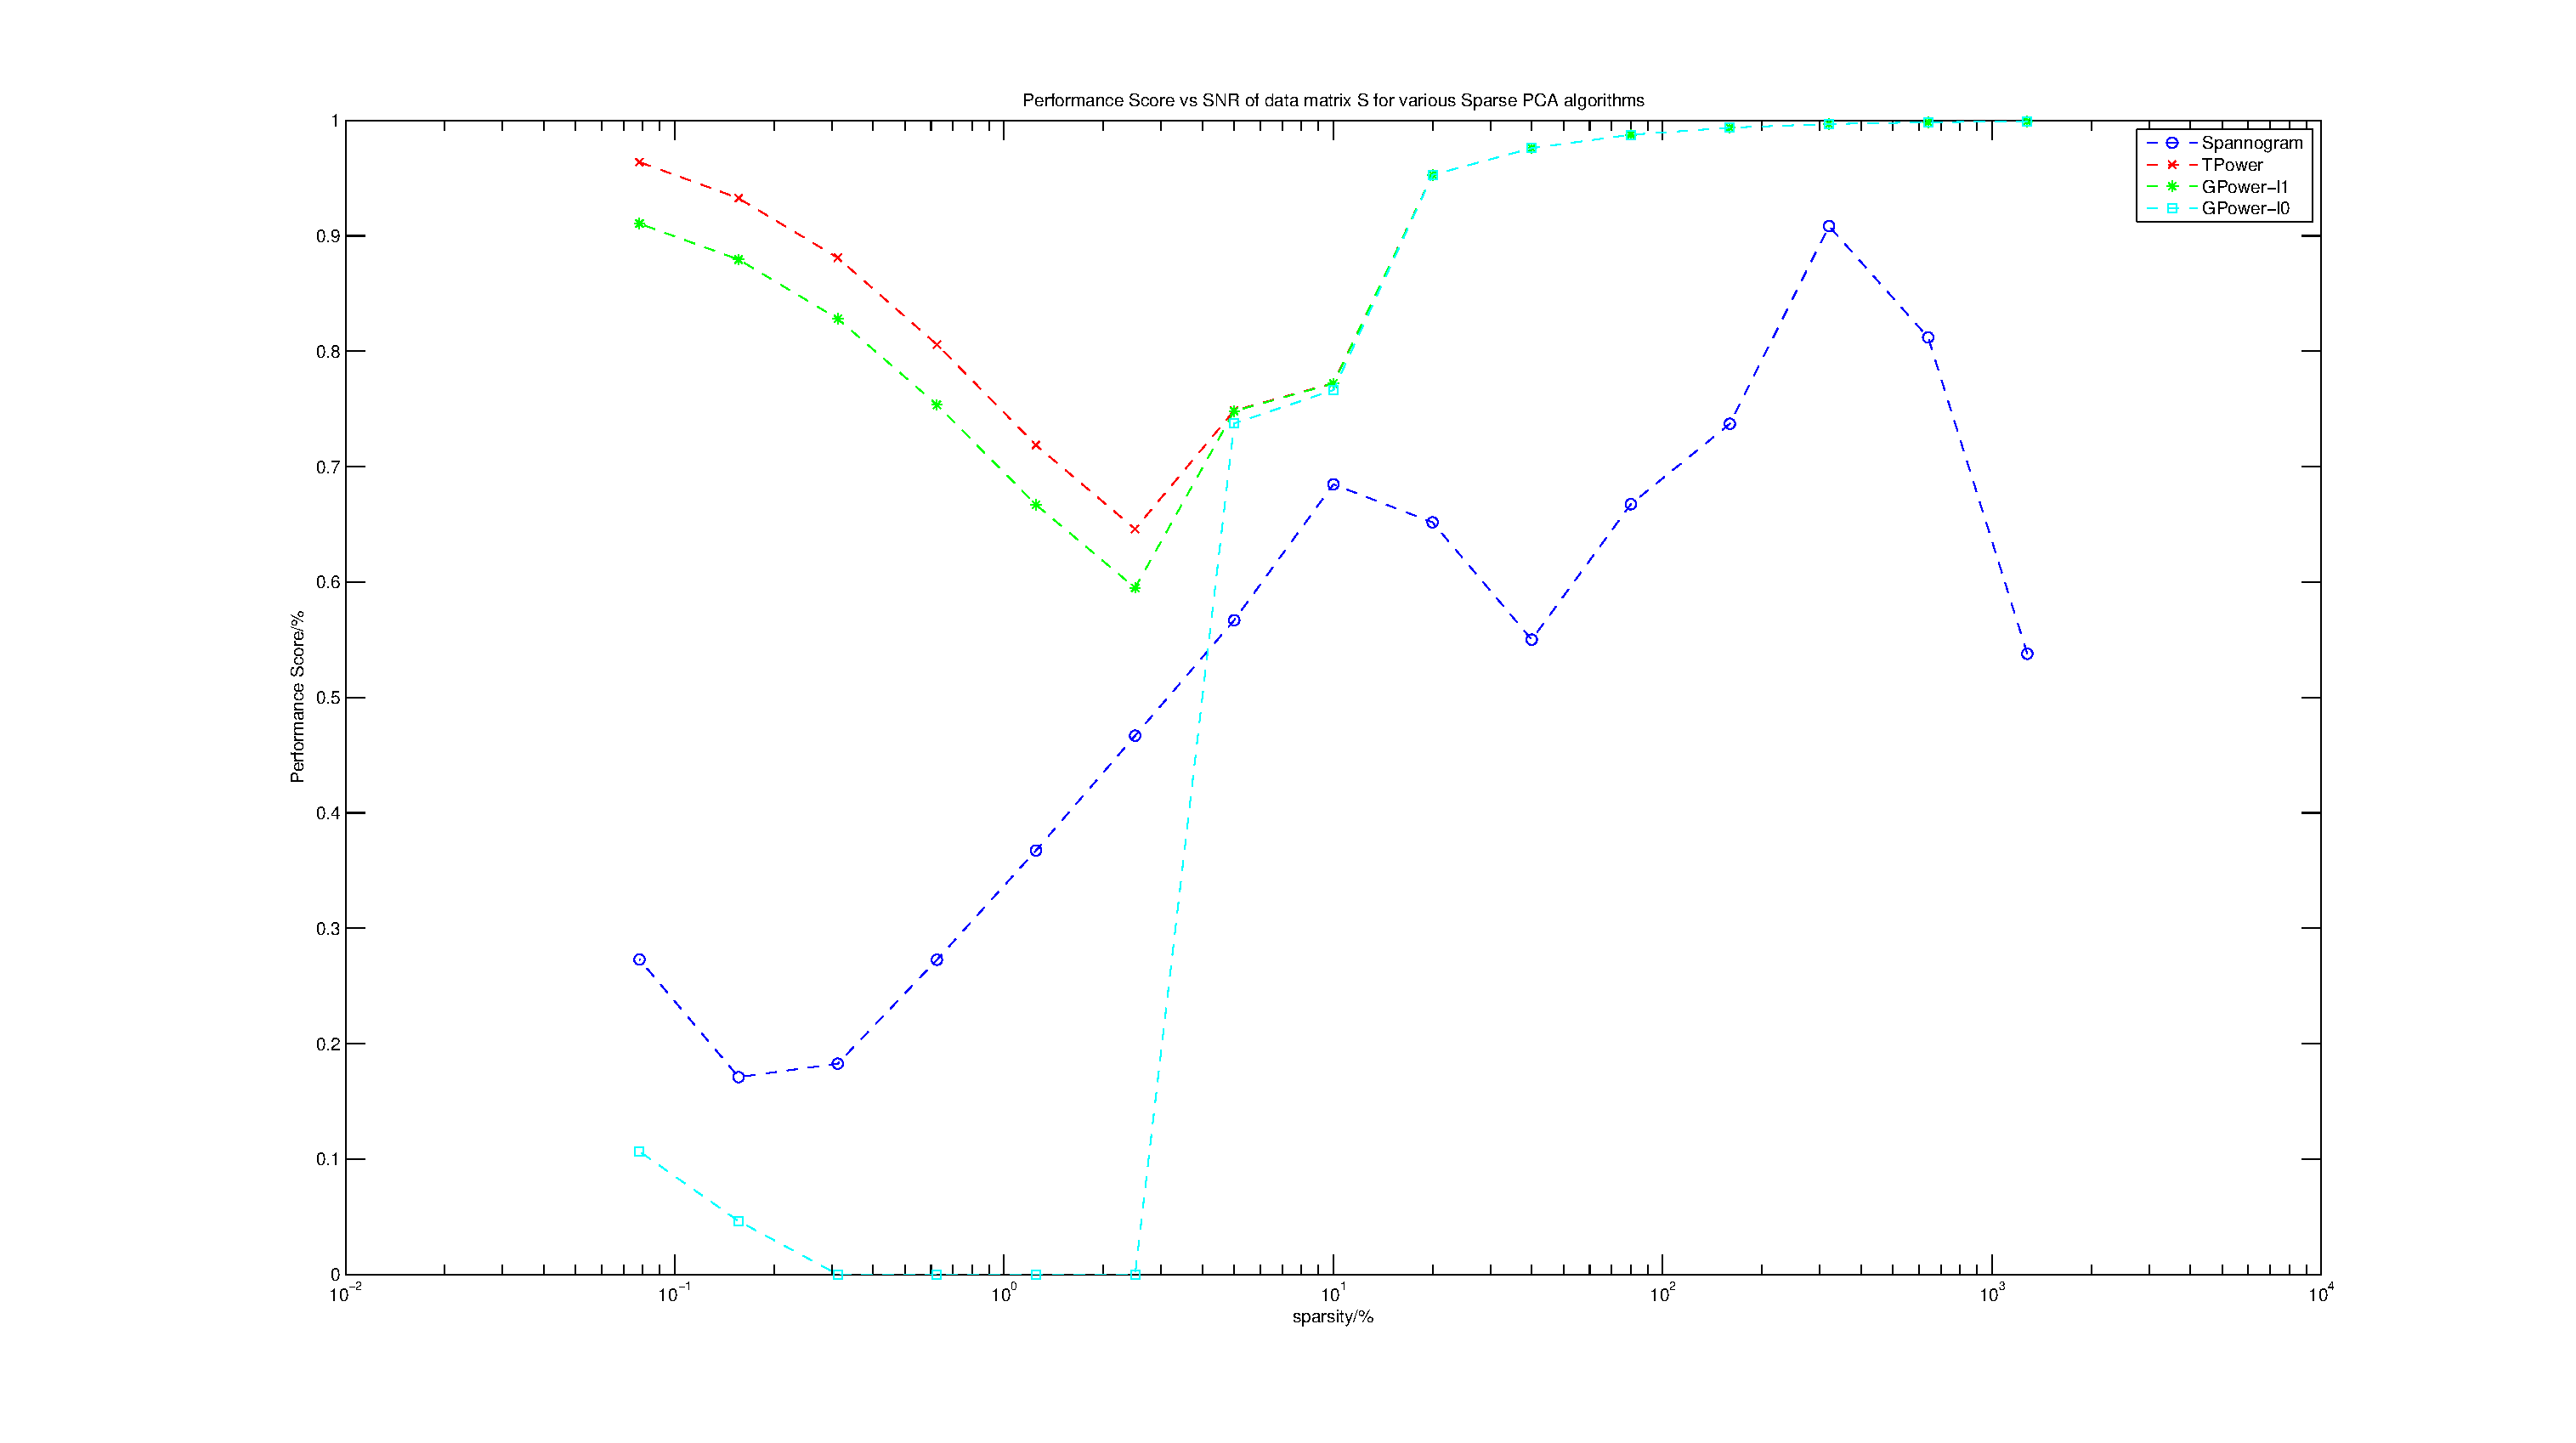
\includegraphics[scale=0.3]{performance_score_vs_snr_5000.eps}
\caption{How the different algorithms perform as the SNR varies for fixed sparsity with $m = 5000$.}
\label{cpev_5000}
\end{figure}

\begin{figure}[H]
\centering
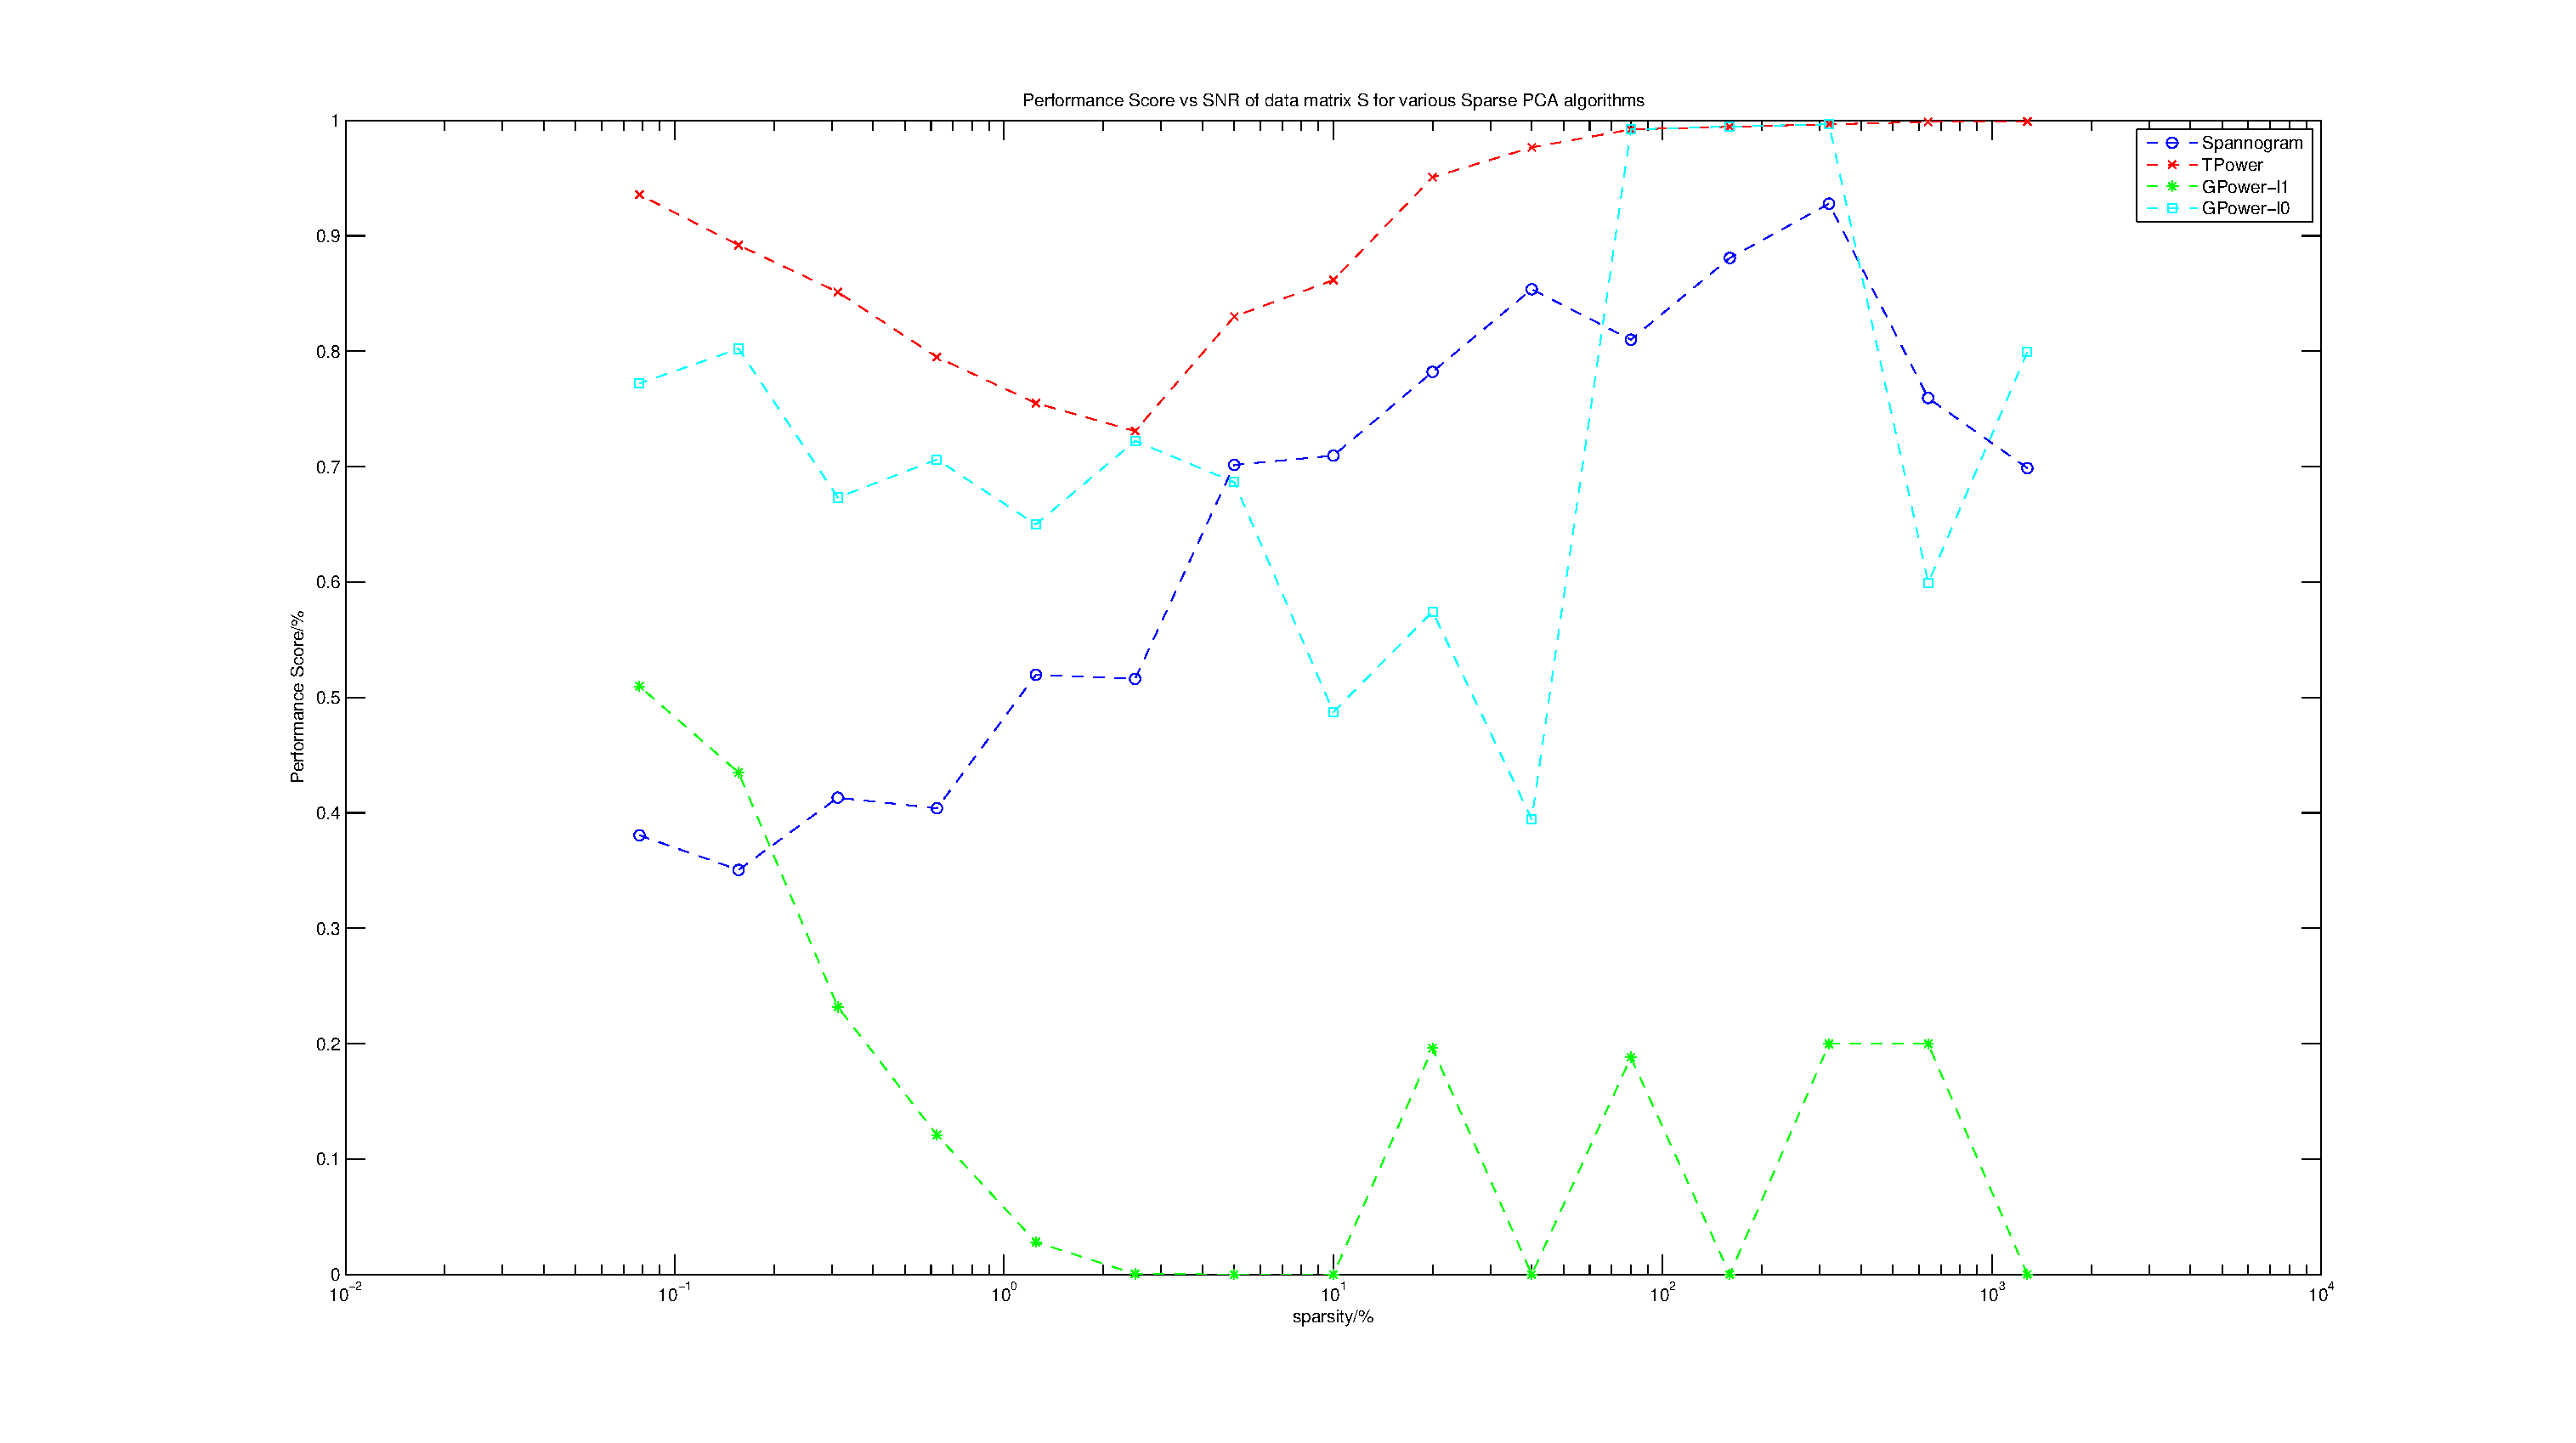
\includegraphics[scale=0.3]{performance_score_vs_snr_10.eps}
\caption{How the different algorithms perform as the SNR varies for fixed sparsity with $m = 10$.}
\label{cpev_10}
\end{figure}

%TODO
It can be seen here that the TPower seems to always outperform the Spannogram PCA algorithm considered in \cite{dimakis}, and by a very significant amount for both cases. The GPower methods sometimes do also, but the problem is that $\rho$ has to be tweaked and tuned for different levels of the SNR (see \cite{GPower}). As is evident in Table \ref{performance_5000}, the TPower algorithm consistently maintains over $64$\% of the variance whereas the Spannogram PCA algorithm has a minimum of $17$\%. This is further shown in Table \ref{performance_10}, where the number of data points is even lower and again there is a gap of roughly $10$\% between the two, TPower being best. When the GPower methods do work, however, they basically match the TPower algorithm. Added to this, the Spannogram algorithm has a computation time of over 300 times any of the other three algorithms, the other three being of comparable magnitude.

\subsubsection{Testing with Binary Data Matrix $\smat$}
\begin{comment}
 results can be found in testing_sparse_PCA_binary_matrix_different_levels_sparsity_results.mat
\end{comment}
Though the Spannogram algorithm seems to perform the worst in the scenario above, where the covariance matrix has actual sparse eigenvectors, in \cite{dimakis} the authors do not use it on this type of matrix, and for the specific example that is being considered in this paper initially (Twitter data), the data matrix, $\smat$, is a binary matrix, each entry taking only the values in the set $\{ 0, 1\}$. Furthermore, the matrix $\covmat$ is not equal to a conventional covariance matrix (refer to section \ref{covmat}). This test revolves around trying to emulate this scenario. 

The data matrix, $\smat$, is created by adding a one to each entry independent of any other entry with some probability $p_\text{1}$, which is chosen to be $0.05$, which is quite artificial since it very likely that many features will come in packages, since this is essentially what is being searched for. Nevertheless, this is done and then the covariance matrix, $\covmat$, is created as in section \ref{covmat}. The algorithms are then used on this to find the sparse principal components and the performance score is calculated, as previously. The results can be seen in Figure \ref{perf_score_binary_matrix} and Table \ref{performance_bin_data_5000}. In this case, though all algorithms have quite a low performance, the Spannogram algorithm actually performs the best. 


\begin{table}[H]
\center
\begin{tabular}{|l|r|r|r|}
\hline
Algorithm &  Score Max &  Score Min & Average Computation Time/s\\
\hline
  Spannogram-R3&   0.4297&    0.1441&    		9.9996\\
 TPower&   0.4297   & 0.1431   & 		0.0048\\
GPower-$l_1$   & 0.3992  &  0.0000  &  		0.0155\\
   GPower-$l_0$ &  0.1603  &  0.0000 & 		 0.0058\\
\hline

\end{tabular}
\caption{Table showing the average performance of different algorithms for computing sparse principal components of the matrix $\mathbf{A}$ with $m=5000$ for a binary data matrix $\smat$.}
\label{performance_bin_data_5000}
\end{table}

As a further test, the data matrix is created slightly differently. Instead of having all feature's probabilities independent of one another, this time some features are given as correlated. If one of the features in the correlated set is one, then the probability, $p_\text{corr}$, of the rest being one increases drastically, in this case this probability is set to $0.85$. This should give results slightly more relevant to the the scenario of interest since words which are related in some way should appear more frequently together than words that aren't. 

Then different sparsity levels are created by increasing the value of the  $p_\text{1}$, whilst keeping $p_\text{corr}$ constant. The sparsity levels (given as a percentage of how many non-zero elements $\smat$ has) are expected to be slightly higher than $p_\text{1}$ due to the fact that $p_\text{corr}$ will be used occasionally also. 

The features to be correlated are arbitrarily chosen to be feature numbers $1, 2, 31, 39, 40$. 5 have been chosen and the algorithms should all aim to return 5-sparse vectors (for the GPower algorithm this is heuristically set by $\rho$, see \cite{GPower}, and a setting of between 0.3 and 0.5 is used here) corresponding to these. The algorithm is run with $m = 5000$ data points and the $m = 10$ data points is neglected as the relative performance does not seem to change. What can be seen from these results is that both the Spannogram and the TPower algorithm have almost identical results under these circumstances, with the Spannogram algorithm performing slightly better. As the sparsity ranges from roughly $0.05\%$ to $75\%$ both get the exact same score and identical sparse PCs. On the contrary, both GPower algorithms do significantly worse, and this is largely due to the fact that the tuning parameter $\rho$ must be chosen very carefully for a desired sparsity and this makes it very sensitive to changes in the sparsity of $\smat$. When GPower$_{l1}$ does match the other two, however, it has almost the exact same PCs also, with the same sparsity level. The setting that is being considered in this report is with $\smat$ of $1.5\%$ sparsity or less, as detailed in section \ref{sparsity_matrix}. Due to the fact that the Spannogram Algorithm and the TPower algorithm perform best in this range, according to these results, and the fact that a binary matrix is what is actually considered, as is the case in this section, the GPower algorithms will no longer be used and instead the Spannogram and TPower algorithm will be evaluated against one another. 



\begin{figure}[H]
\centering
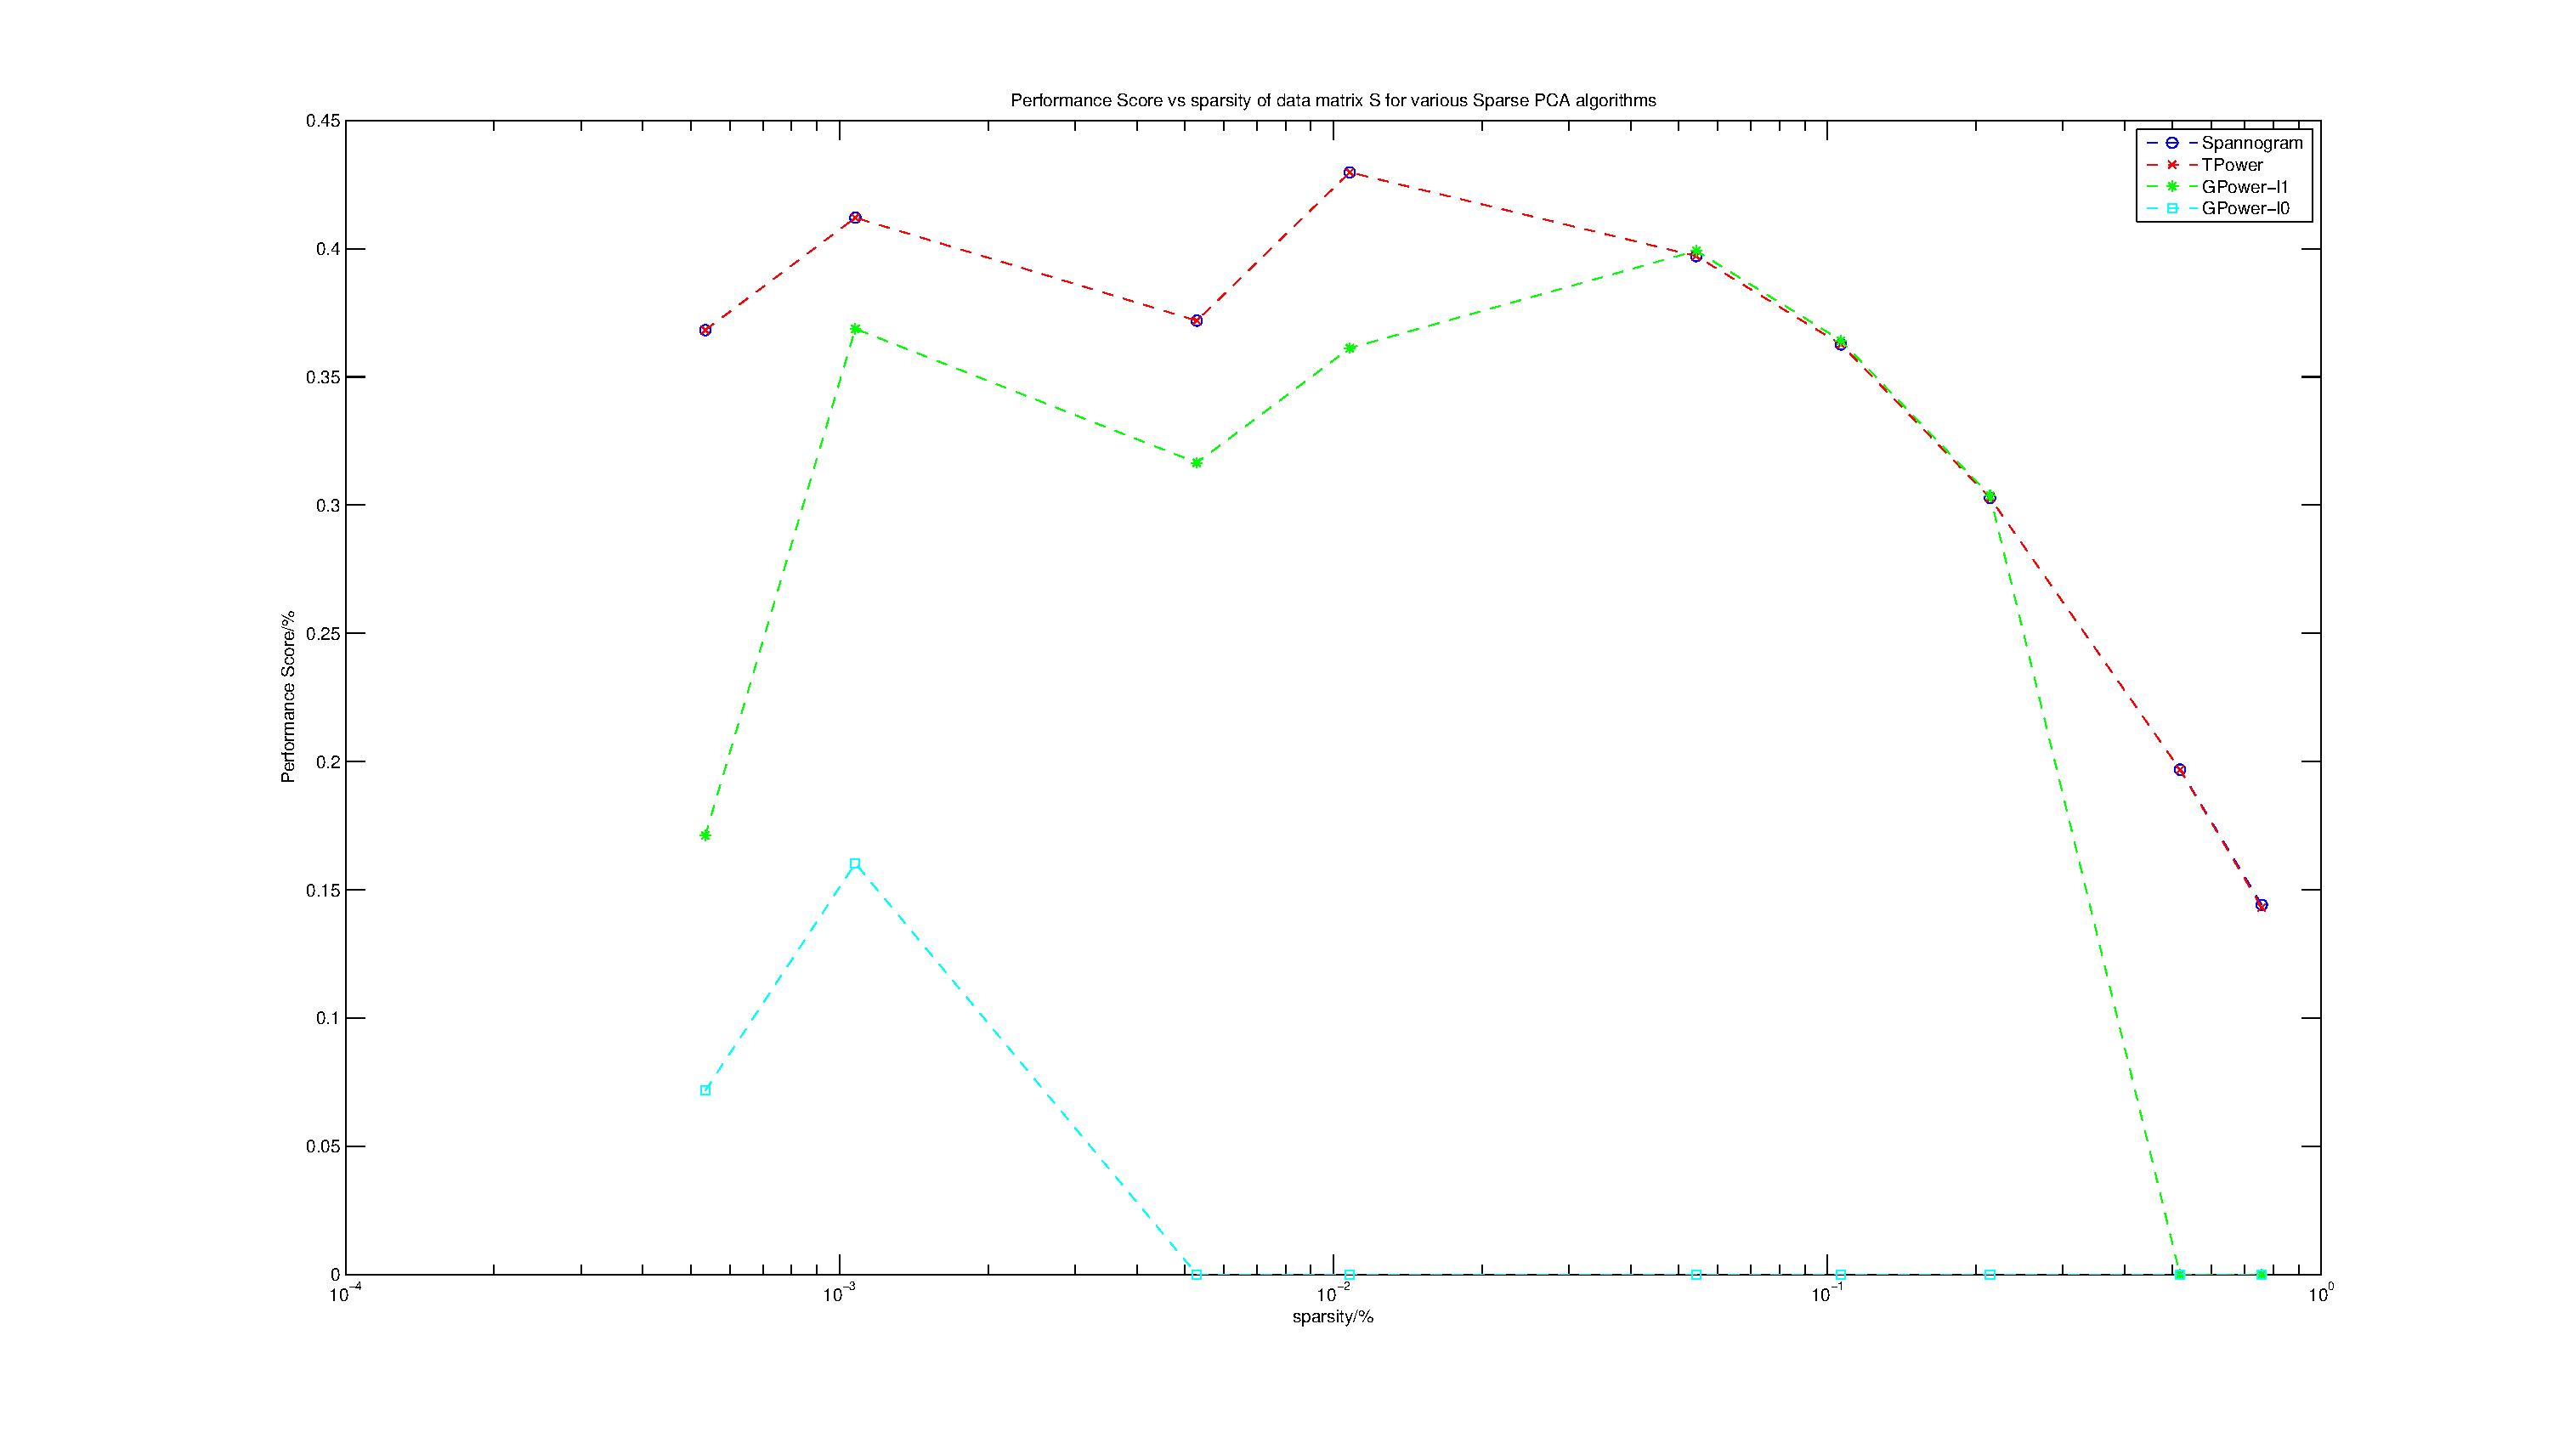
\includegraphics[scale=0.3]{performance_vs_sparsity_5000.eps}
\caption{How the different algorithms perform as the average sparsity varies with $m = 5000$.}
\label{perf_score_binary_matrix}
\end{figure}


\begin{equation*}
\mathbf{\mathbf{v}_1}=
\begin{pmatrix}
0.1564\\
0.1718\\
0.1567\\
0.1545\\
0.1554\\
0.1577\\
0.1556\\
0.1576\\
0.1557\\
0.1571\\
0.1559\\
0.1585\\
0.1563\\
0.1566\\
0.1569\\
0.1561\\
0.1565\\
0.1563\\
0.1552\\
0.1562\\
0.1566\\
0.1570\\
0.1552\\
0.1568\\
0.1565\\
0.1586\\
0.1554\\
0.1563\\
0.1583\\
0.1568\\
0.1716\\
0.1586\\
0.1579\\
0.1576\\
0.1572\\
0.1559\\
0.1568\\
0.1568\\
0.1695\\
0.1698\\
\end{pmatrix}
\end{equation*}
Something to note is how the actual eigenvector, $\mathbf{v}$, of $\covmat$ is not sparse at all, which is the difference with the previous section in which the algorithms were trying to retrieve the actual sparse eigenvectors. This is why the Spannogram performs so badly in comparison to the other algorithms. 

%TODO  Explain further

\subsection{Comparing TPower and Spannogram PCA}
\label{comparison}
% Results can be found in spannogram_vs_tpower.mat and then looking at the metrics matrix.
To test the performance of the TPower algorithm and the Spannogram algorithm for the Twitter data gathered for the period 25/09/2012 - 26/09/2012 different sparseness are considered for the principal components and the first two principal components are evaluated by the algorithms. 

The set of words that is desired can be seen in Table \ref{murder_8} as these are the words that represent the most significant event that happened in the period of time considered (as calculated using the hollow matrix describe in section \ref{covmat}). Let this set be referred to as $\mathbb{S}$. Other sparse principal components do emerge, however, they mostly arise as words that may occur quite frequently together but do not actually represent a specific event, for instance ``happy'' and ``birthday'' appear quite  a lot, but do not necessarily represent a single event. Furthermore, when $k$ increases the new words included do not actually give any more information and so have not been included in the table, but for the analysis $k$ will increase to 12 for completeness.

\begin{table}[H]
\center
\begin{tabular}{| c l |}
\hline
Index & Word \\
\hline
12 & please\\
827 & officers \\
889 & murders \\
240 & following\\
783 & fallen \\
756 & recent\\ 
190 & police\\
787 & colleagues\\
\hline
\end{tabular}
\caption{The dominant 8-sparse principal component for 25/09/2012 - 26/09/2012 calculated using the Spannogram PCA algorithm.}
\label{murder_8}
\end{table}

The way the two algorithms will be evaluated against one another is by running them on the data iteratively and upon each iteration increasing the desired number of non-zero elements in the principal components, $k$, by 1. The desired outcome for each is that on every iteration, a subset of $\mathbb{S}$ is recovered and that the performance score for both be monotonically increasing with $k$. Furthermore, any principal component extracted must have a higher eigenvalue (and therefore higher CPEV) than any of the following principal components extracted. 

\begin{figure}[H]
\centering
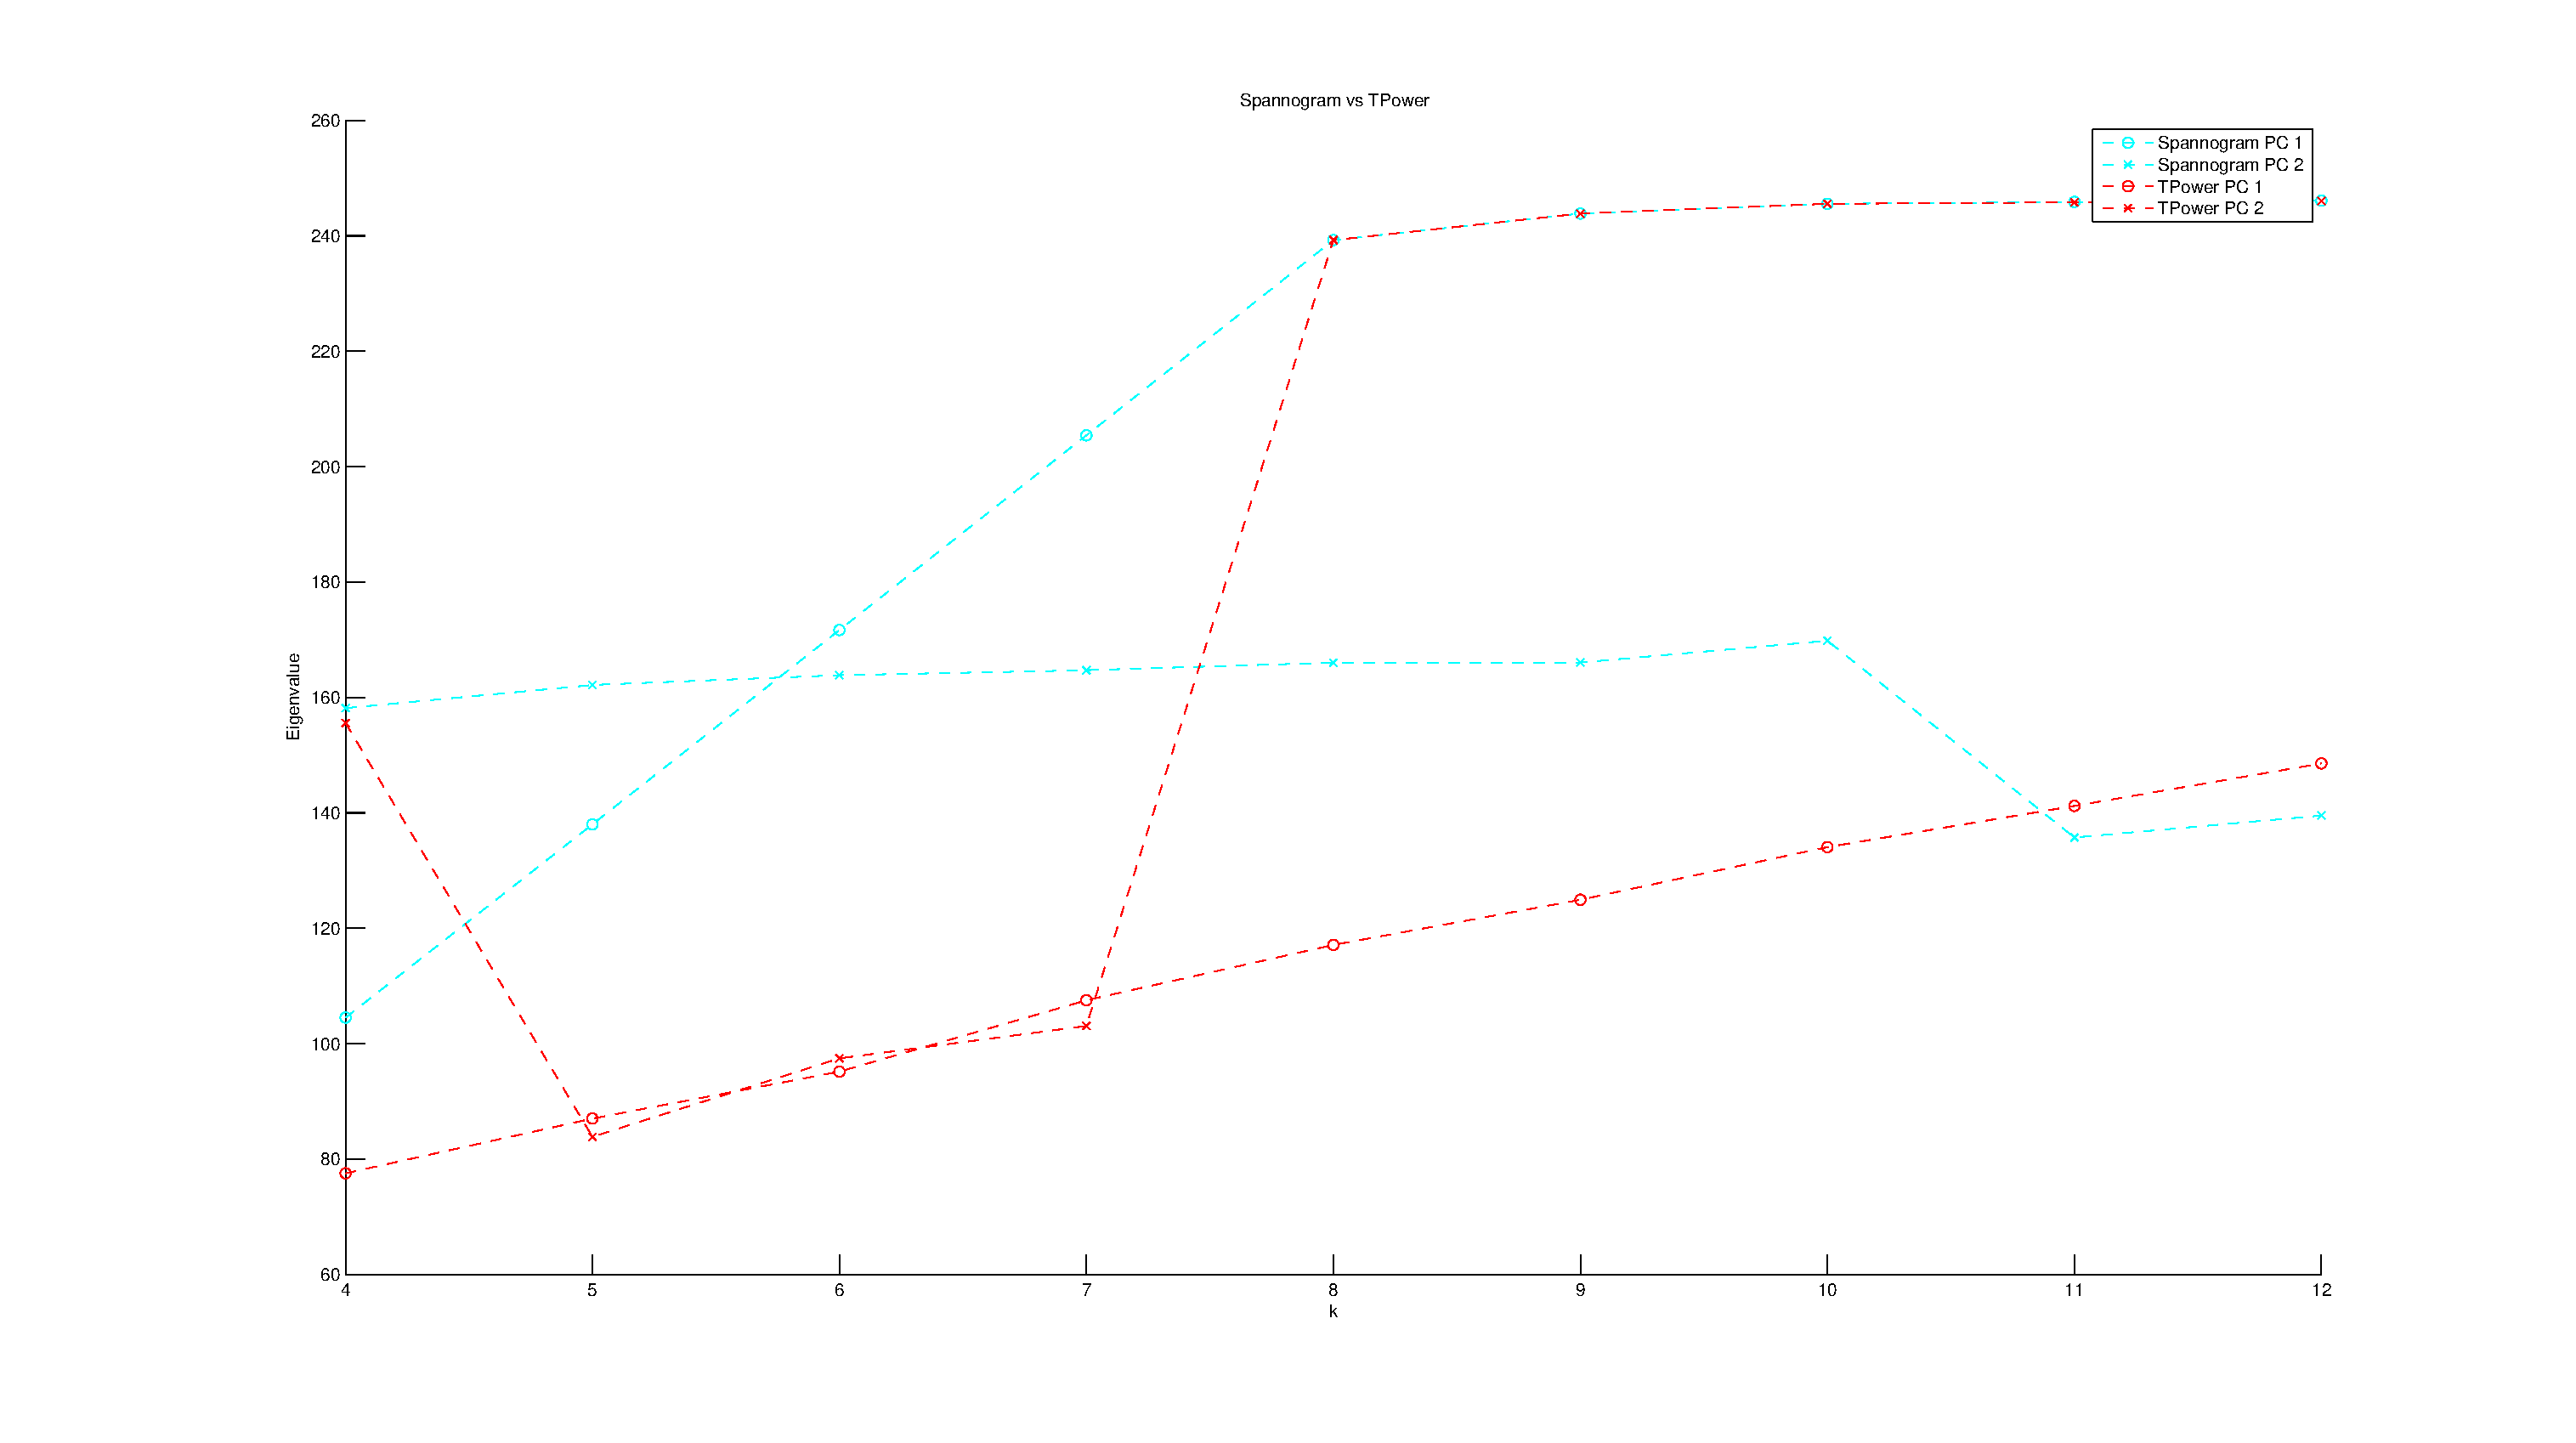
\includegraphics[scale=0.3]{Spannogram_vs_TPower_k.eps}
\caption{How the explained variance of the principal components varies with the number of non-zero elements in it, $k$.}
\label{explained_var_graph}
\end{figure}

\begin{comment}
%TODO Explain these results against the criteria stated above. 
- Explain how the 2nd PC for TPower gives a higher variance than the first => bad.
- Explain how for TPower not monotonically increasing until k = 8.
- Explain how spannogram always wins.
\end{comment}

\subsection{Conclusion}

%TODO Fix this again
From the findings it appears that the Spannogram PCA algorithm is more accurate and more consistent in terms of the principal components found in the context of finding events in Twitter data, using the defined objective function. 

As shown in Figure \ref{explained_var_graph} the Spannogram PCA algorithm either outperforms the TPower algorithm or does equally well for both principal components (PC). The interesting thing to note from these is that (a) the TPower algorithm is not consistent in its findings, as can be seen by its second PC, which initially has quite a high value and one of the words from $\mathbb{S}$, but after increasing the value of k, fails to have any of the words in $S$ until k becomes 8, at which point it contains all the words in $S$. The Spannogram algorithm on the other hand consistently keeps its previously calculated words and, upon each increase in sparsity, it just adds an extra word. Furthermore, for the Spannogram algorithm, the explained variance associated with both PCs monotonically increase with respect to the sparsity, which is not the case for the TPower algorithm, the red line in the figure increasing the most since it is associated with the words in Table \ref{murder_8}.

These results are completely contrary to the results found in section \ref{testing}. This is largely believed to be accounted for by the structure of the $\mathbf{S}$ matrix in each case. In \cite{truncpower}, it is suggested that if the matrix $\mathbf{A}$ has sparse or approximately sparse eigenvectors then the TPower algorithm can approximate these, which has as its underlying assumption that the true eigenvectors are themselves almost sparse. The Spannogram algorithm does not make this assumption at all. Instead it finds PCs which may not represent the true PCs in any way whatsoever. For instance, getting the true leading eigenvector of $\mathbf{A}$, it turns out to be that 44 of the 3000 words are at least $50\%$ the magnitude of the highest magnitude element in the leading eigenvector. Which may be approximately sparse considering that this is a small fraction of 3000 but it is still much larger than just 4 to 8 words. In this context, the vector is not sparse at all. This is a crude measurement for ``approximately'' sparse but it is merely for illustration purposes. 

It can be concluded that the Spannogram PCA algorithm performs best when the matrix $\mathbf{A}$ does not actually have sparse PCs in the conventional sense but still has sparse components that can model the variance in the data fairly well. However, after the sparsity increases beyond 8, they appear to perform almost equally. On the other hand, the speed of the TPower algorithm is much better than that of the Spannogram PCA algorithm, by a factor of approximately $10^3$, which should be taken into account when developing an application which requires quick computation time. In any case, either one of these should be used to suit the needs of the application and the trade-off between speed and accuracy should be the deciding factor. 
\clearpage



\section{Application Implementation}
\begin{comment}
From the results found so far, it can be seen that different algorithms may prove to be more effective than the Spannogram PCA algorithm. This means that further work has to be done evaluating other algorithms, as those found in \cite{shen}, \cite{zou}, \cite{daspremont}, \cite{asteris} 
and any others, and finding which ones would be best to use for the specific scenario. It may be the case that the Spannogram PCA algorithm performs worse with a conventional covariance matrix, but performs much better on the matrix $\mathbf{S}^T\mathbf{S}$ which is used on the Twitter data, so this also must be researched further. 

The algorithms will be evaluated, as done in section \ref{testing}, and a performance score will be given to them. Then the same algorithms will be evaluated on the Twitter data, as in section \ref{testing_twitter} and the results will be compared to see whether algorithm performances depend on the data structure. The results of this research will lead to an algorithm being chosen and this algorithm will be examined further so as to find any improvements that could be made to it, or a couple of algorithms could be merged to keep the benefits of both. Consideration will also be given to the data at hand to see if the structure could be exploited further, as the authors of \cite{dimakis} attempt to do. Upon completion of this, the new algorithm will also be evaluated similarly to before, to determine whether the alterations have had a positive effect.

If along the way any other difficulties arise, due to scalability issues or the data structure, these will first be tackled and the changes will also be evaluated. 

\end{comment}

\subsection{Big Data Streaming Application}
In this section, methods to ensure computational feasibility are considered, and an algorithm is created to make this possible under high volume data applications in which the rate of data is very large while the number of variables considered is comparatively low i.e. $m >> n$. As already mentioned previously, there are roughly 40k Tweets on average per day in London, which corresponds to quite a small volume which can be processed all in one go, but suppose that the world were to instead be considered, which would give a rate of about 58 million Tweets per day, then clearly a method would need to be considered to be able to process all that data in a streaming fashion. 

Needless to say, this would only work if there were an actual trending topic in the whole of the population. 
\subsubsection{Concerns}
The idea is to stream Twitter data and to be able to automatically detect whether an event is taking place online. This could be used, for instance, as a web application to find events in certain areas or for marketing purposes. 

There are various methods of doing this in an online fashion and it opens many doors for research, but the basic approach is to have a sliding window of some number of Tweets, which depends on the application and the size of the geographical location being considered, to perform the Sparse PCA algorithm on it and to see how the principal components change over time. There are various considerations that must be addressed, including:
\begin{itemize}
\item How large should the window size be?
\item By how many Tweets should the sliding window increment by?
\item How can an event be detected based on the change in the principal components. 
\item How could this scale?
\end{itemize}

\subsection{Streaming Procedure}
The algorithm to be used in this scenario is the TPower algorithm. This is because, though it sometimes is less accurate, it is typically a factor of $10^3$ faster than the Spannogram PCA algorithm and so for a large data streaming application, the trade-off of accuracy for speed is worth it. 

\subsubsection{Algorithm}
%TODO Change this whole subsubsection
%TODO Must add to the algorithm that the PC words must be added to the bag of words. 
%TODO Must remove the part which states that not the whole cov matrix will have to be calculated because it is untrue. There will be new words therefore the old covariance matrix will no longer be valid. 
The algorithm can be described as follows:

\RestyleAlgo{boxruled}
\LinesNumbered
\begin{algorithm}[H]
\KwData{The Stream of Tweets}
\KwResult{The Sparse Principal Components for each batch of Tweets}
\While{Streaming} {
//  (a) Get the new data\\
$D_\text{new} \leftarrow $ New Batch of $K$ Tweets;\\
// Pop the old data off the queue, $\mathbf{Q}$\\
$D_\text{old} \leftarrow \mathbf{Q}(1:K)$;\\
// Shift the queue of data. W is the sliding window size.\\
$ \mathbf{Q}(1:W-K) \leftarrow \mathbf{Q}(K+1:W) $\\
// Put the new data at the end of the queue\\
$ \mathbf{Q}(W-K+1:W) \leftarrow D_\text{new}$\\
// (b) Get the new Bag-Of-Words\\
$ B = \text{getBagOfWordsFromData}(D)$\\
// (c) Populate the new data matrix \\
$\smat = \text{getMatrixFromDataAndBagOfWords}(D, B)$\\
// (d) Calculate the new co-occurrence matrix\\
$\covmat = \smat\tp \smat - \text{diag}(\smat\tp \smat) $\\
// (e) Compute new Sparse PCs \\
$[\mathbf{V}_\text{new}, \mathbf{\Lambda}_\text{new}]$ = ComputeSparsePCA($\covmat_\text{new}$);\\
// Save new data\\
ListOfSparsePCs.Append($\mathbf{V}_\text{new}$)\\
ListOfEigenvalues.Append($\mathbf{\Lambda}_\text{new}$)\\

}
\end{algorithm}

\subsection{Time Per Calculation}
As streaming is being considered, which is an online process, it is very useful to see how long each calculation of a sparse principal component takes. It is also useful to know how this time varies, on average, with the size of the window being considered.
\subsubsection{Complexity}
%TODO Check complexity of TPower
The complexity of the final algorithm can be split into various parts and can be calculated as the complexity given as a number of operations per section. The sections are labeled in the comments of the algorithm above as (a)-(e). The loading of the new Twitter data (a) is merely linear $O(m)$, where $m$ is the number of Tweets per window. Loading the bag of words (b) has a time complexity of $O(N\log(N))$, where $N$ is the total number of words from the Tweets. This is simply because the algorithm first builds a dictionary of all the words and then sorts them to get the top $n$. Populating the matrix (c) has a time complexity of $O(mp)$, where $p$ is the average number of words in a single Tweet. Building the co-occurrence matrix (d) is of the order $O(mn^2)$ and the final Sparse PCA algorithm depends on which algorithm is used, but in this case is an iterative algorithm. 

It should be noted that these complexities represent different types of operations and therefore a combined complexity has not been given.
 
\subsubsection{Proportion of Time Spent in Each Portion}
%TODO Explain this
\begin{figure}[H]
\centering
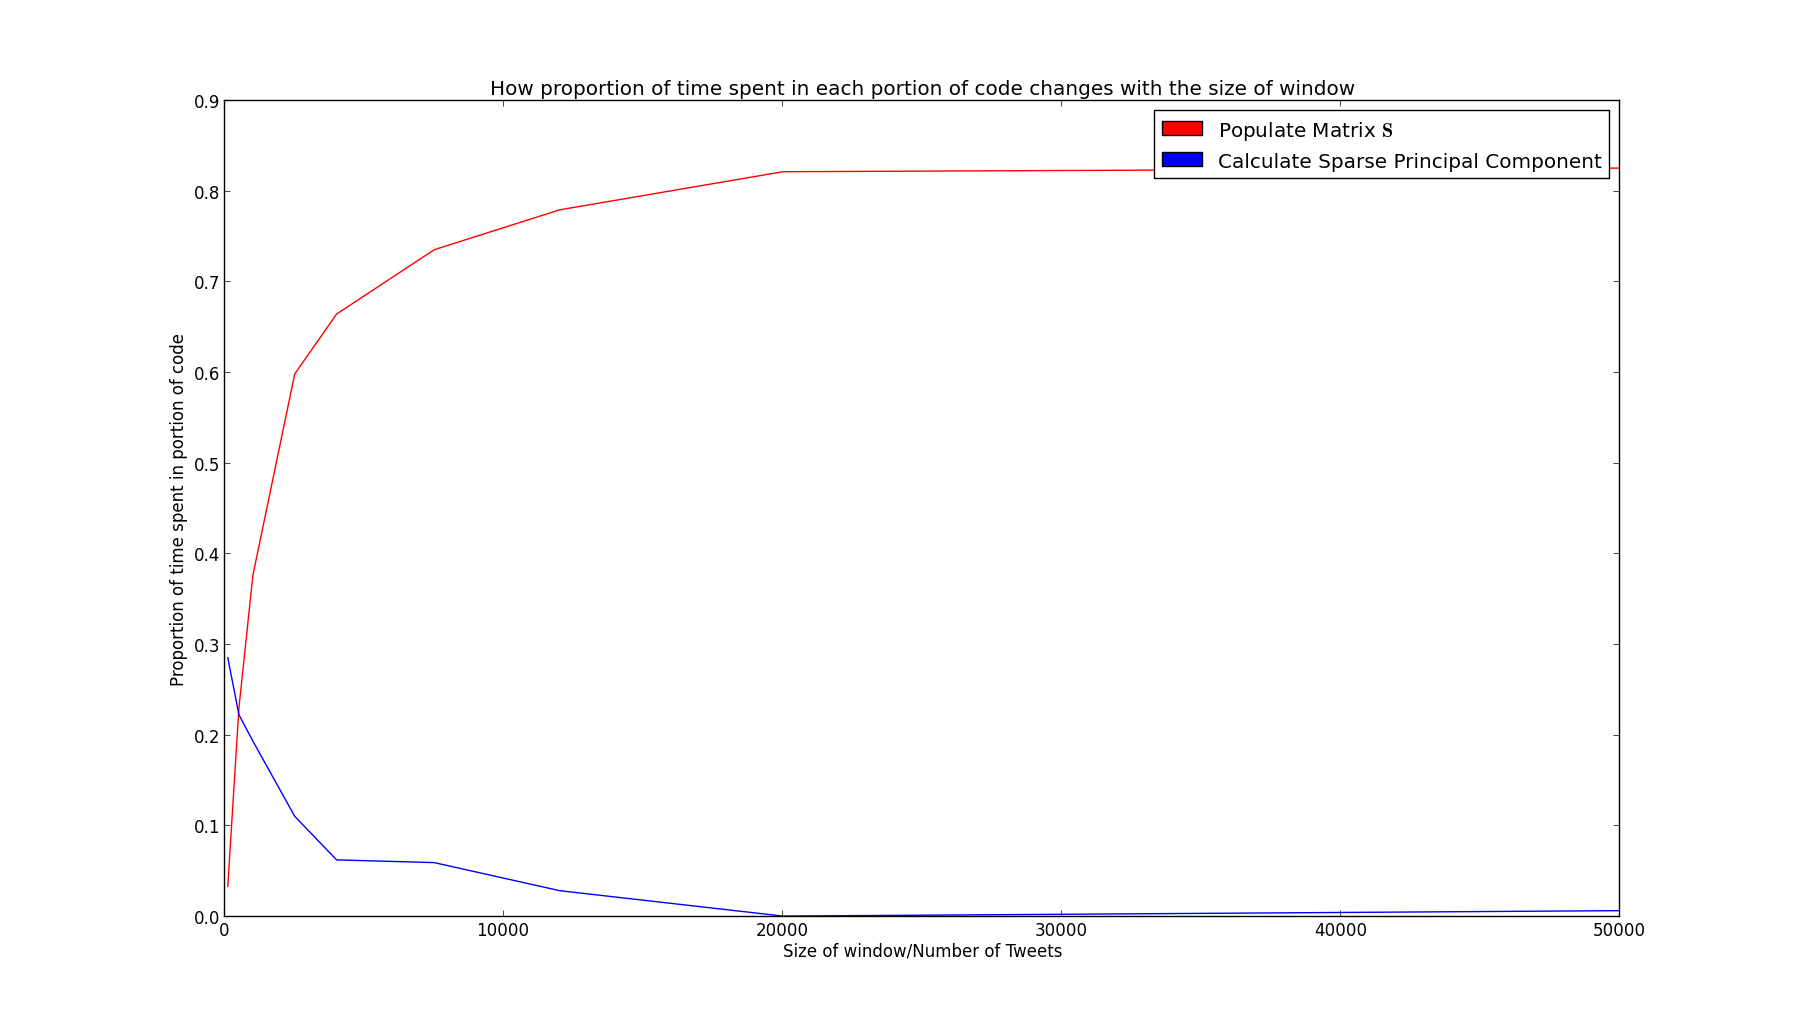
\includegraphics[scale=0.30]{proportion_time.png}
\caption{The proportion of the total time it takes per iteration to perform the calculation of the sparse principal component and to populate the matrix $\smat$ vs the number of Tweets per window. This is done using a Bag-Of-Words of size 3000.}
\label{proportion_time}
\end{figure}

As it can be seen in Figure \ref{proportion_time}, for a Bag-Of-Words with 3000 words, which is the setting that has been chosen and has been used up until this point in this paper, the proportion of time spent in the section of the algorithm to populate the matrix $\smat$ grows with the number of Tweets and starts to level off at about 0.8. The opposite is true for the TPower algorithm, which uses less of the proportion of the total time as the number of Tweets increases in a given window. For most practical scenarios, the size of the window, $m$, will be greater than 1000 and therefore most of the time will be spent in the populating of $\smat$. This means that trying to optimise this piece of code would increase performance significantly.
%TODO Finish this 
\subsubsection{The Bottle Neck: Time to Construct $\smat$}

This is investigated by creating the data matrix $\smat \inintmxn$, keeping $n$ constant but varying the number of Tweets, $m$. The co-occurrence matrix is then calculated and a sparse principal component is calculated using the algorithm. Since the co-occurrence matrix being considered is actually the same size in all cases ($n \times n$), the time to execute the Sparse PCA algorithm should not change, however, the time to build the data matrix does change, and should vary linearly with $m$. The results can be seen in Figure \ref{time_matrix_construction}.

\begin{figure}[H]
\centering
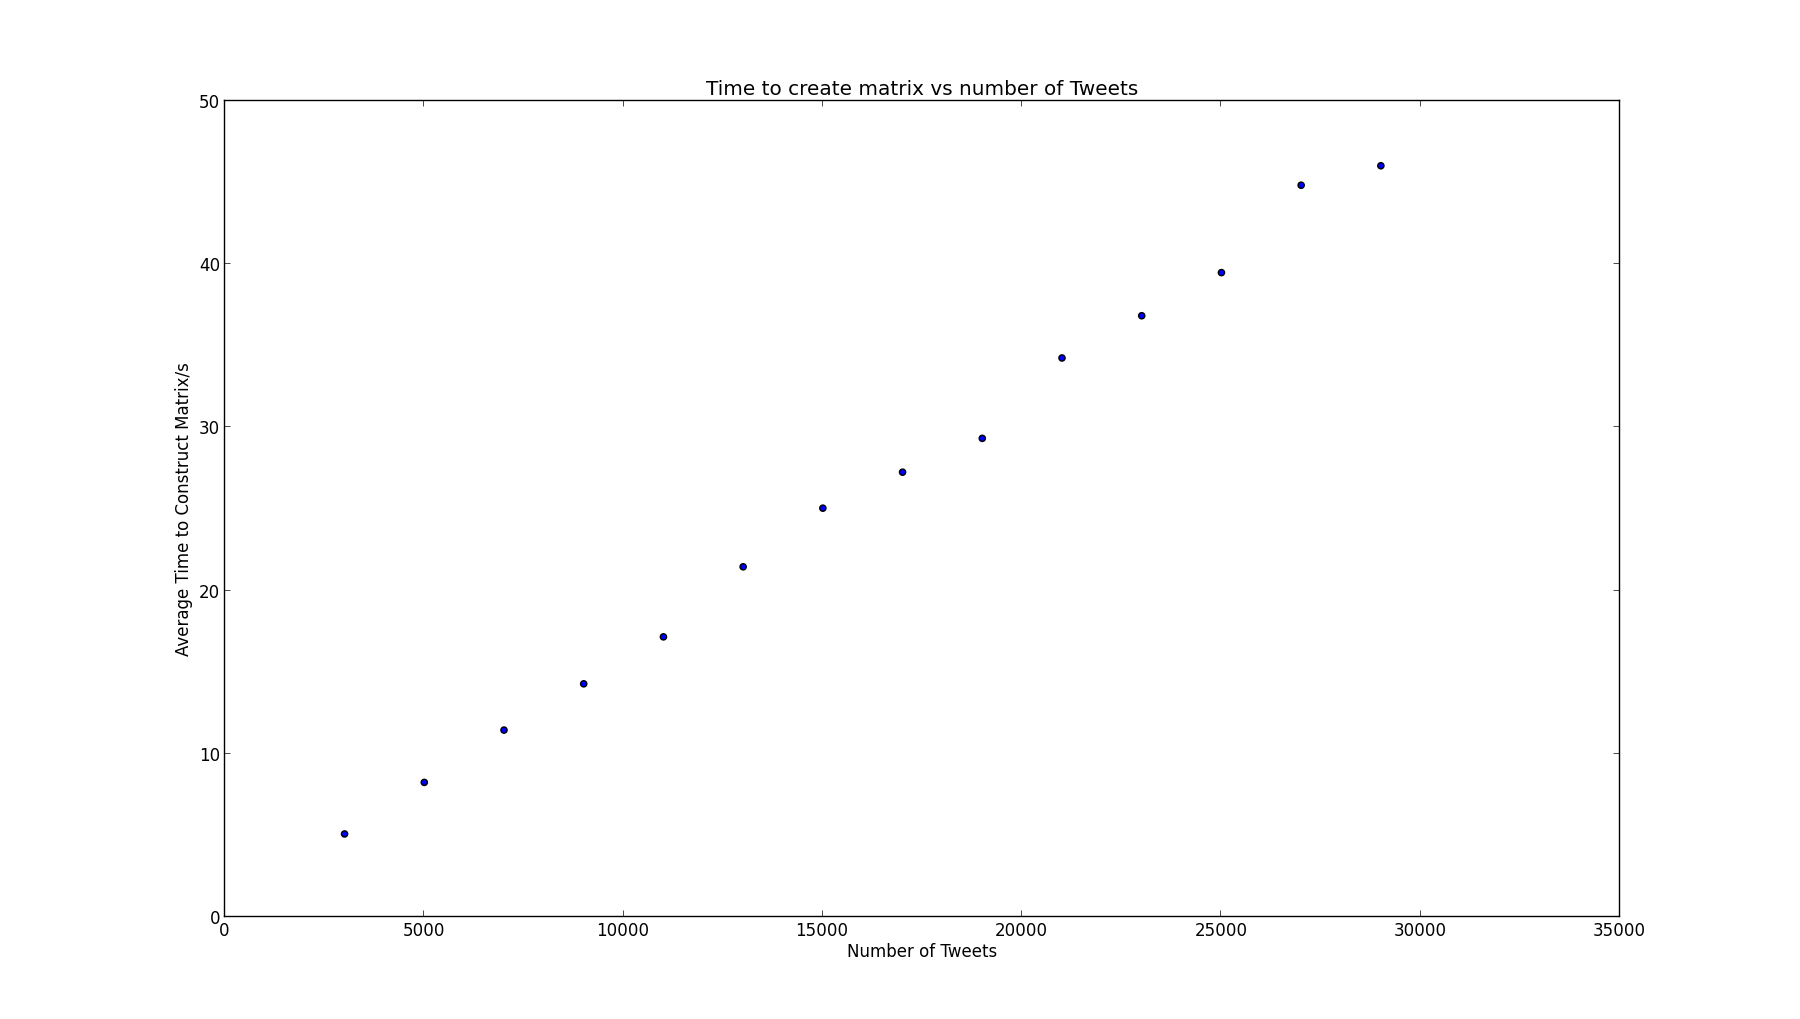
\includegraphics[scale=0.30]{Time_Matrix_Construction.png}
\caption{The time it takes to create the data matrix $\smat$ against the number of Tweets.}
\label{time_matrix_construction}
\end{figure}

It can be noted that, indeed, the time for construction of the matrix does vary linearly with $m$, the number of Tweets. What this means is that by keeping the product of the number of Tweets per window and the number of windows per period of time constant, the time of calculation should also stay the same. For example, one could calculate a data point every hour with a $2x$ number of Tweets or calculate a data point every half an hour with $x$ Tweets and the total time would be approximately the same.

\subsection{Parameter Choices}
%TODO
\begin{comment}
Mention the following:
- How to choose the size, k, of the batches.
- How to choose the threshold for the CPEV. 
- How to choose the size of the window size, W. 
- How to choose max number of trending topics.
- Explain how events are detected. 
- Show that for a different data set that this is not optimal.
\end{comment}
As aforementioned there are many parameters that must be chosen, each needing to be chosen based on the volume of the Tweets and the scale of the geographical location that is being considered. An attempt is made in this section to show how different parameters affect the results and why. This is done using a subset of the data, namely the same data used in section \ref{comparison} in the period 25/09/2012 - 26/09/2012, which contains the event regarding the death of the two police officers.

\subsubsection{The Number of Tweets}
%TODO Analyse this further
%TODO Try to do with a very small amount of points e.g. 100 so that it also doesn't work
 
What is first considered is how the window size (the number of tweets considered upon each iteration) and the shift size (by how many Tweets the window advances upon completion of each iteration) affect the results of the streaming application. Four different cases are considered for the window size and shift size and the results can be seen in Figures \ref{testing_app_20000}, \ref{testing_app_15000} and \ref{testing_app_10000}, \ref{testing_app_4000}, \ref{testing_app_80}. 

As it can be seen, varying the window size has a very significant effect on the detection of events. Having too large a window means that the matrix considered is large and therefore principal components associated with certain events may be hidden by the noise, since the noise factor increases with the number of Tweets being considered. To illustrate this, consider the toy example of there being 10000 Tweets over the span of 1 day, where 5 of these contain exactly the same words and the rest are randomly generated. If the window size is exactly 5, these words should come out as the supports of the principal components for the appropriate window, however, if all 10000 are considered, these would be unlikely to be detected as principal components at all as they only count for a small proportion of the data matrix. On the other hand, decreasing  the window size means that the eigenvalue changes can be seen more gradually and that the time resolution of the events is finer meaning that events can be pinpointed in time much more effectively. Furthermore, the higher the resolution, the more the events that can be found (up to a reasonable extent i.e. having a window size of one Tweet would not return anything useful apart from some words from that one Tweet). The problem with having a window size that is too small however, is that small insignificant events also appear. For instance, in Figure \ref{testing_app_80} it can be seen that close to the end another event is detected. However, this ``event'' is based purely on the fact that many people retweeted a Tweet that someone wrote regarding a celebrity Ariana Grande but which was not actually an event but which for a very small period of time was quite prevalent in the Twitter feed. Therefore, by decreasing the window size too much, these micro-events can also creep in and distort results. 

In all scenarios, the algorithm is more than fast enough to carry out the necessary calculations, since in even in the fastest rate scenario considered, a calculation is needed about once every 15 seconds, which for the matrix size, is within the bounds to be able to keep up with real time calculations.

\begin{figure}[H]
\centering
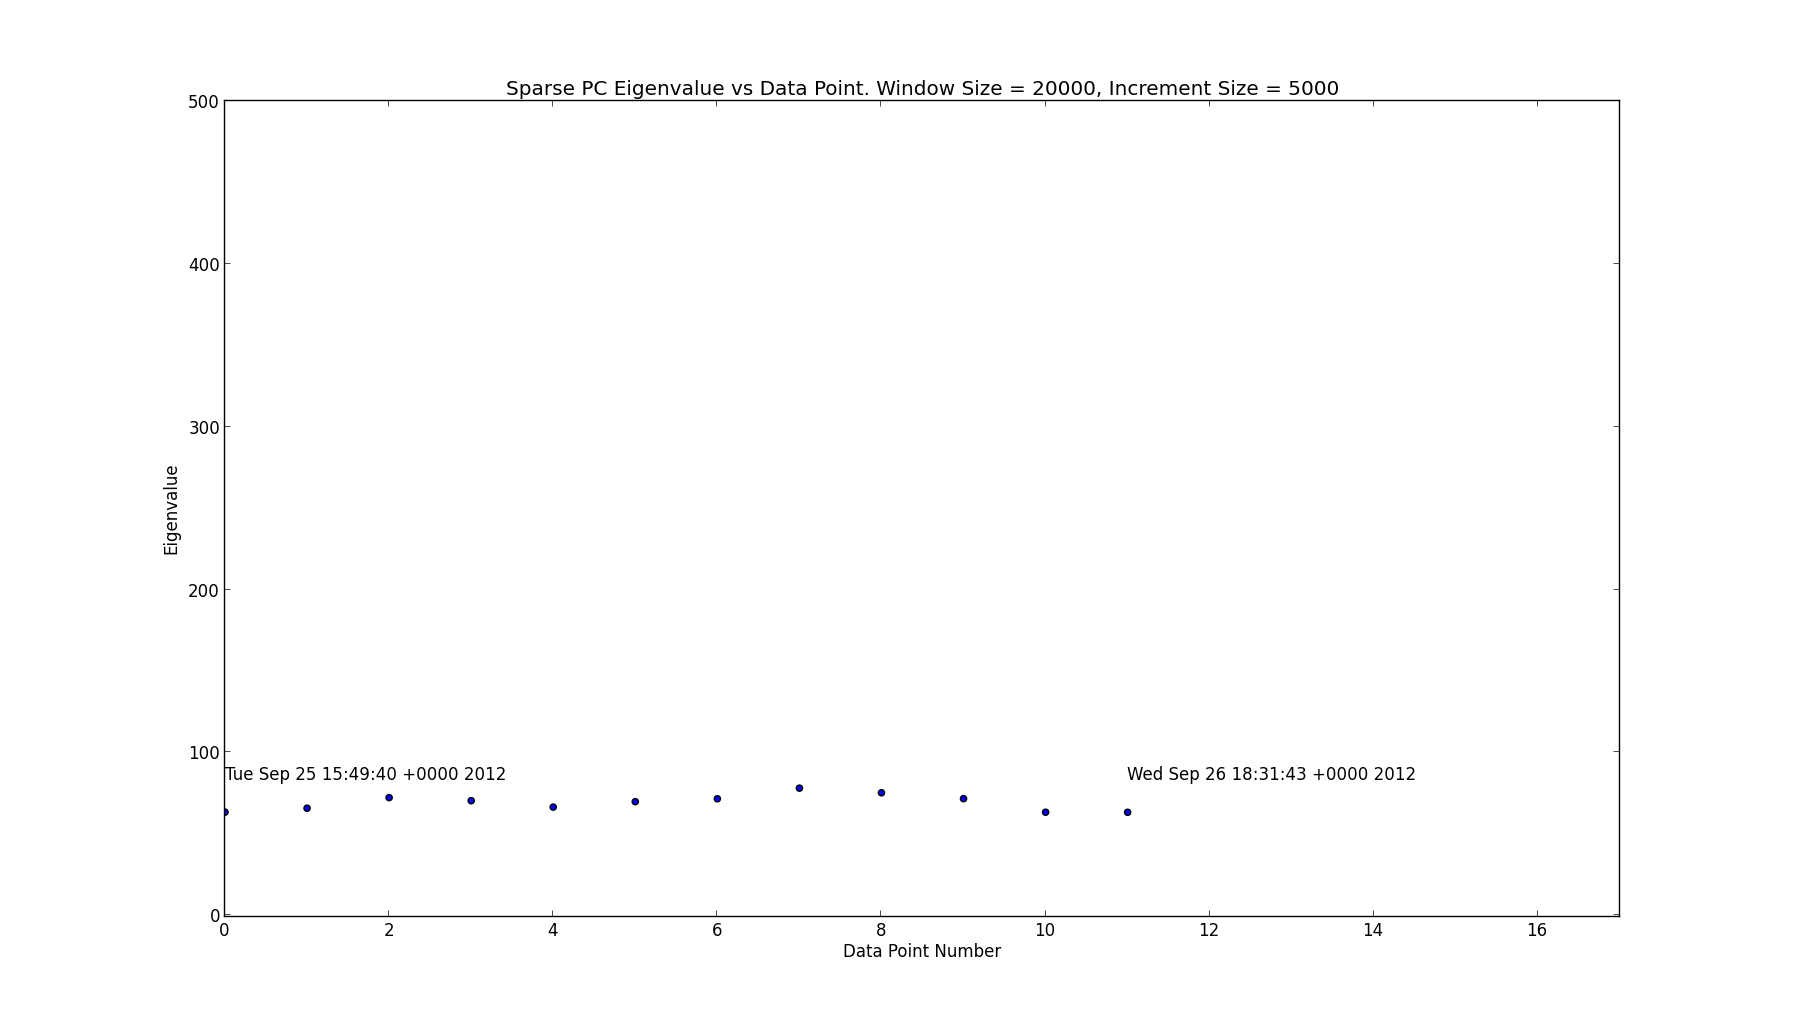
\includegraphics[scale=0.25]{Testing_Streaming_App_20000_5000.png}
\caption{Testing the streaming application with a window size of 20000 Tweets and a shift of 5000 Tweets for each data point. The start and end dates are labeled on the graph. This corresponds to doing a calculation roughly every 2 hours. The window size in this case corresponds to about 6.4 hours of Tweets. The event is completely missed out in this case. }
\label{testing_app_20000}
\end{figure}

\begin{figure}[H]
\centering
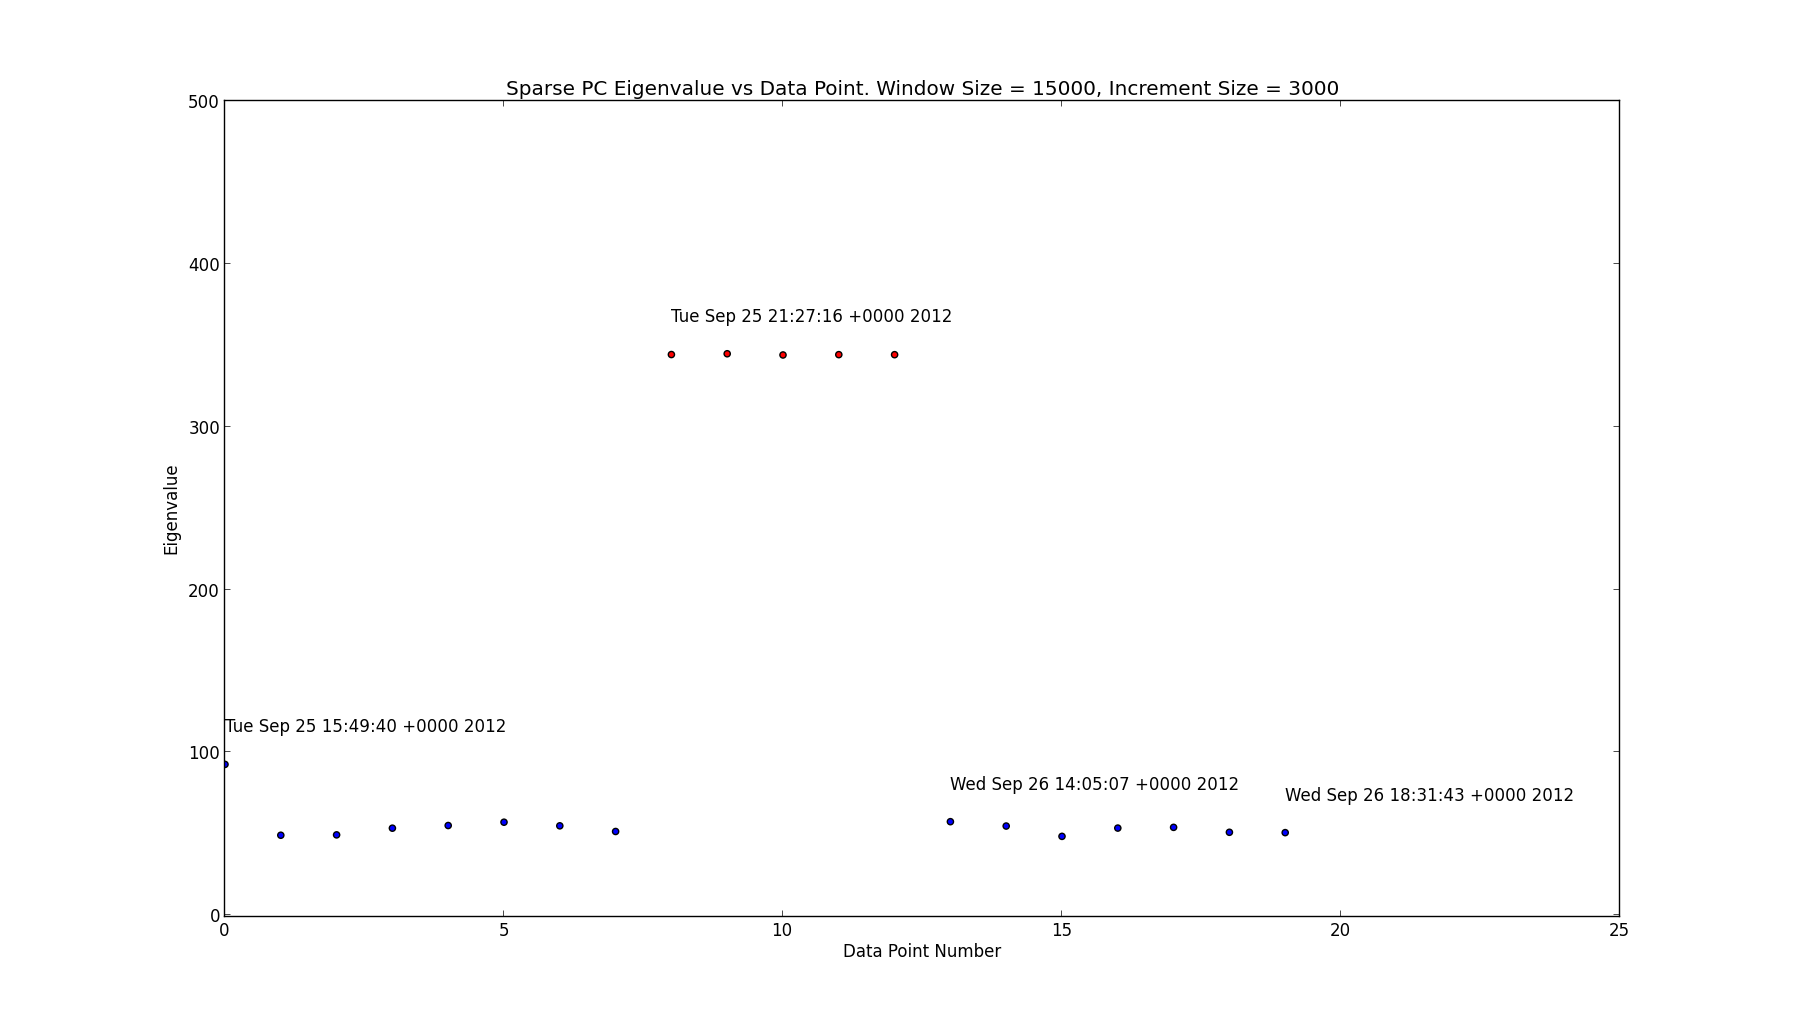
\includegraphics[scale=0.25]{Testing_Streaming_App_15000_3000.png}
\caption{Testing the streaming application with a window size of 15000 Tweets and a shift of 3000 Tweets for each data point. The red points indicate points in which an event has been detected. The start and end dates and times are labeled on the graph, as well as the start and end dates and times of an event. This corresponds to doing a calculation roughly every 1 hour 20 minutes. The window size in this case corresponds to about 4.8 hours of Tweets.}
\label{testing_app_15000}
\end{figure}

\begin{figure}[H]
\centering
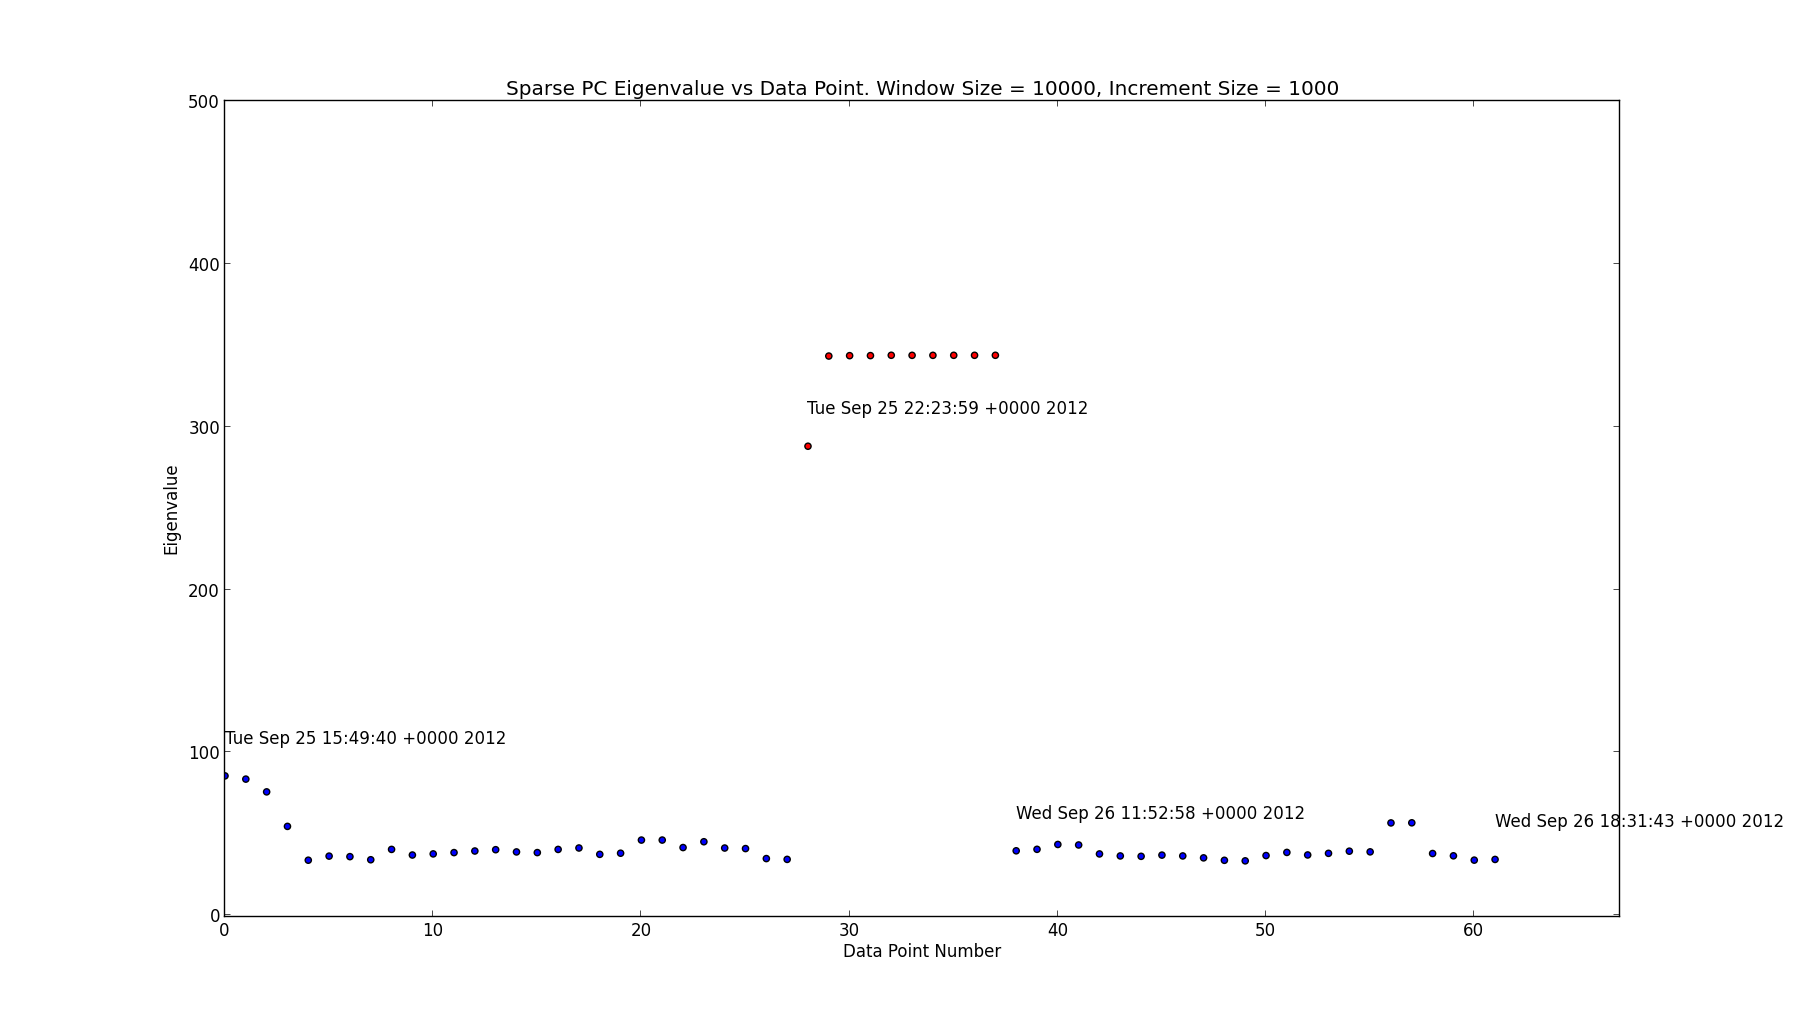
\includegraphics[scale=0.25]{Testing_Streaming_App_10000_1000.png}
\caption{Testing the streaming application with a window size of 10000 Tweets and a shift of 1000 Tweets for each data point. The red points indicate points in which an event has been detected. The start and end dates are labeled on the graph, as well as the start and end dates and times of an event. This corresponds to doing a calculation roughly every  25 minutes. The window size in this case corresponds to about 3.2 hours of Tweets.}
\label{testing_app_10000}
\end{figure}

\begin{figure}[H]
\centering
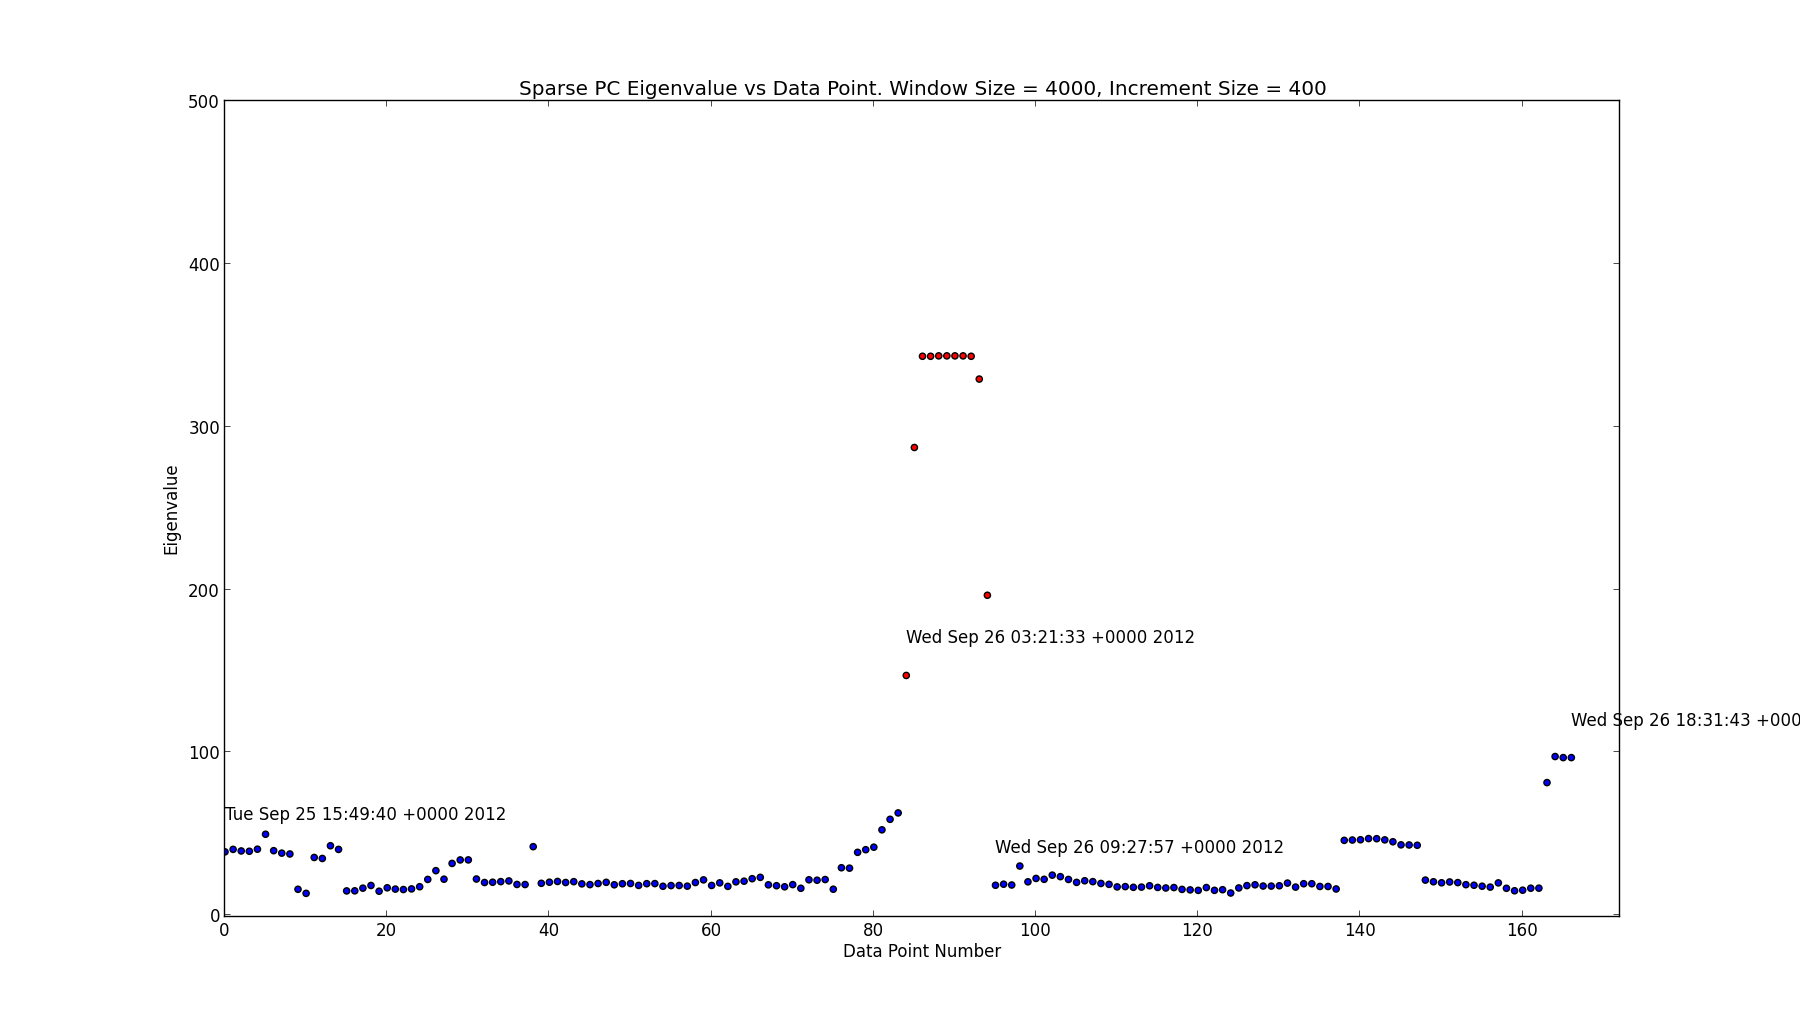
\includegraphics[scale=0.25]{Testing_Streaming_App_4000_400.png}
\caption{Testing the streaming application with a window size of 4000 Tweets and a shift of 400 Tweets for each data point. The red points indicate points in which an event has been detected. The start and end dates are labeled on the graph, as well as the start and end dates and times of an event. This corresponds to doing a calculation roughly every  10 minutes. The window size in this case corresponds to about 1.3 hours of Tweets.}
\label{testing_app_4000}
\end{figure}


\begin{figure}[H]
\centering
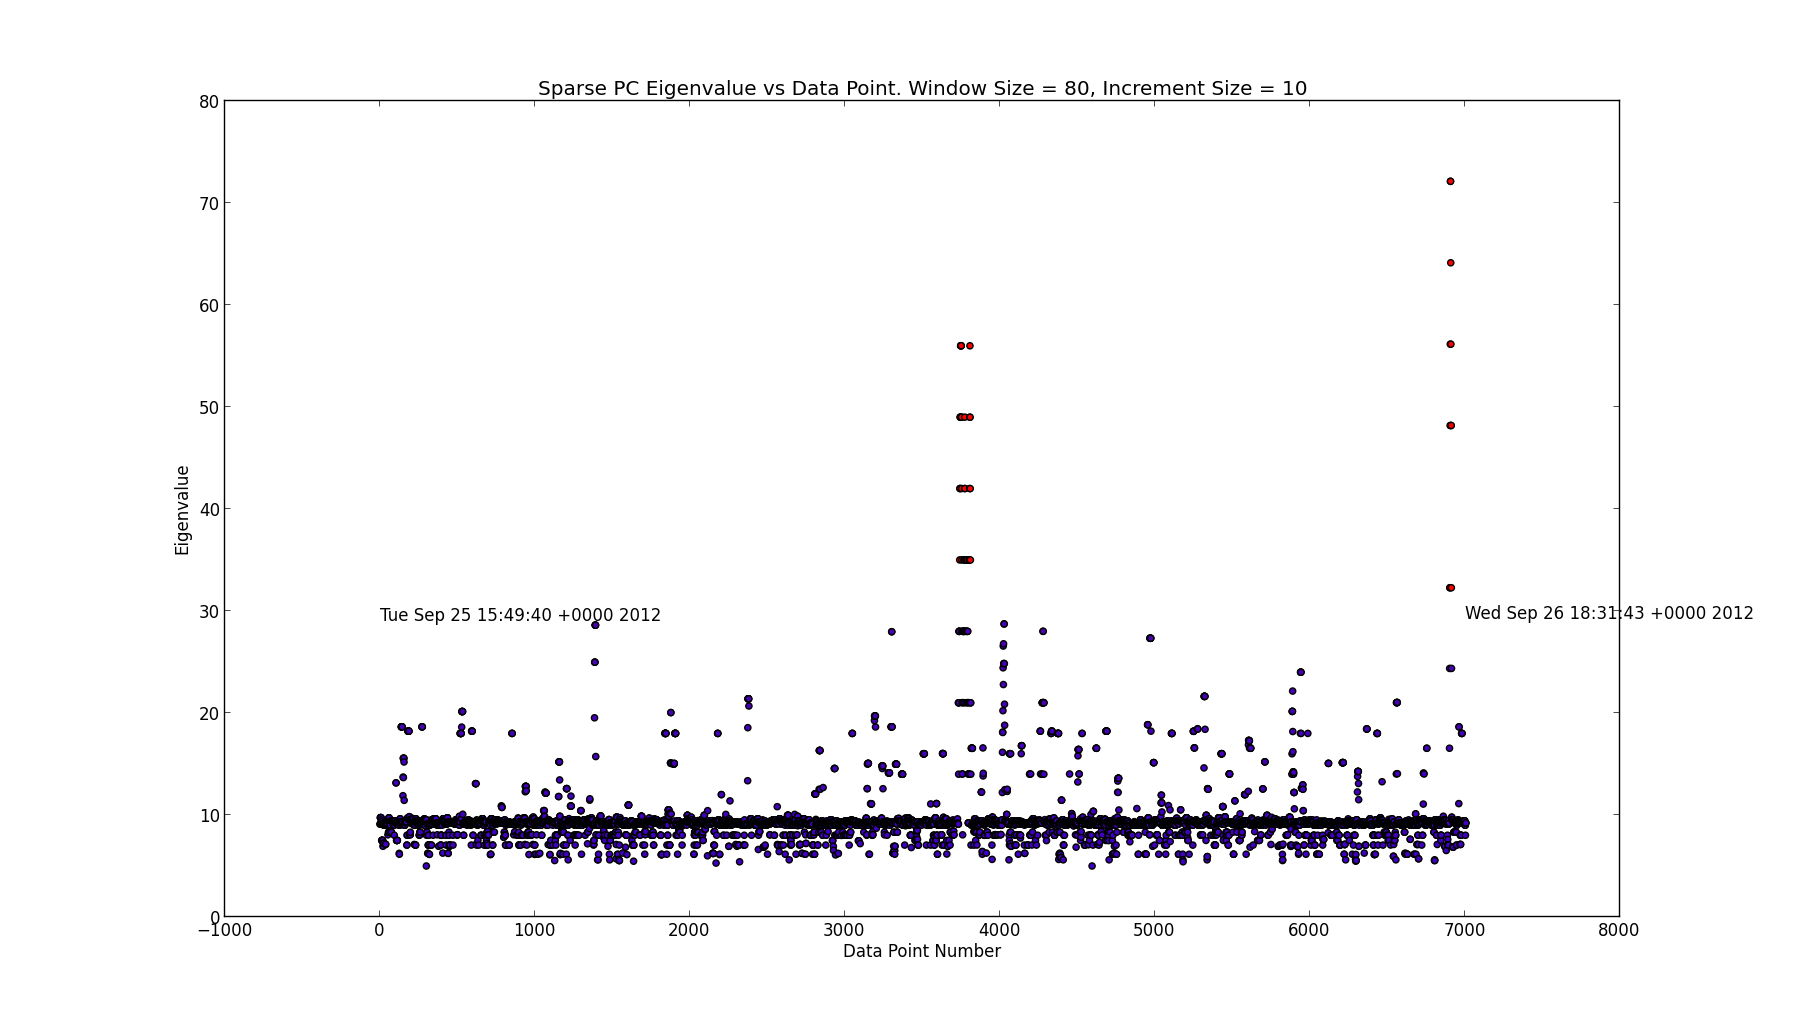
\includegraphics[scale=0.25]{Testing_Streaming_App_80_10.png}
\caption{Testing the streaming application with a window size of 80 Tweets and a shift of 80 Tweets for each data point. The red points indicate points in which an event has been detected. The start and end dates are labeled on the graph, as well as the start and end dates and times of an event. This corresponds to doing a calculation roughly every  15 seconds. The window size in this case corresponds to about 90 seconds of Tweets.}
\label{testing_app_80}
\end{figure}

\subsubsection{Event Detection Variable}
\label{event_detection}

The method used to detect events is quite simple and intuitive, yet very effective. The basic principle is that given that there is not an event, the eigenvalue associated with the first principal component should be relatively low, but when an event takes place, this should increase. The parameter choices in this case are quite ad hoc and depend on quite a few factors, including the size of the matrix and the number of Tweets considered. Therefore, for each different streaming rate and geographical location, a different model must be trained. 

%TODO Check if citation is correct
One way of mapping a scalar to a probability is to use the logistic function \cite{bishop}, given as

\begin{equation}
p(\lambda_i)= \frac{1}{\left( 1 + e^{-(w_0 + w_1\lambda_i)}\right)},
\label{logit}
\end{equation}

where $p(\lambda_i)$ is the probability of the data point associated with the eigenvalue $\lambda_i$ signifying an event and $w_0$ and $w_1$ are the parameters to be estimated. 

The way the parameters are estimated is by taking a set of $\lambda_i$ values, each with a label indicating the probability of how likely it indicates an event. Then by rearranging \eqref{logit} above, it can be seen that

\begin{equation}
y(\lambda_i) = \ln\left( \frac{p(\lambda_i)}{(1-p(\lambda_i))}\right) = w_0 + w_1 \lambda_i,
\end{equation}
therefore, by solving the equation 

\begin{equation*}
 \mathbf{\Lambda}\mathbf{w} = \mathbf{y} ,
\end{equation*}
where the $i$th row of $\mathbf{\Lambda}$ is equal to $\left(\begin{matrix}
1 & \lambda_i
\end{matrix}  \right)$, the $i$th element of $\mathbf{y}$ is equal to $y(\lambda_i)$ and $\mathbf{w} = \left(\begin{matrix} w_0   &w_1\end{matrix}\right)^T$, the parameters $w_0$ and $w_1$ can be estimated in the least squares sense. 

Clearly, the solution to this equation is

\begin{equation*}
\mathbf{w} = \left( \mathbf{\Lambda}^T \mathbf{\Lambda}\right)^{-1} \mathbf{\Lambda}^T\mathbf{y}.
\end{equation*}

With the parameters calculated, all one must do to get the probability of a point being associated with an event is to plug in the value of $\lambda_i$ into equation \eqref{logit}. 

One estimation of the function using a very small number of data points can be seen in Figure \ref{lambda_scatter}. It can be seen that the points in the range of $\lambda \in [100, 250]$ have quite a loose correlation to the probability of an event, however, outside this range it is almost certain that an event has not taken place if $\lambda < 100$ and almost certain that an event has taken place if $\lambda > 250$. For a more accurate solution a much larger number of data points should be considered more densely populating the $\lambda$ axis.

\begin{figure}[H]
\centering
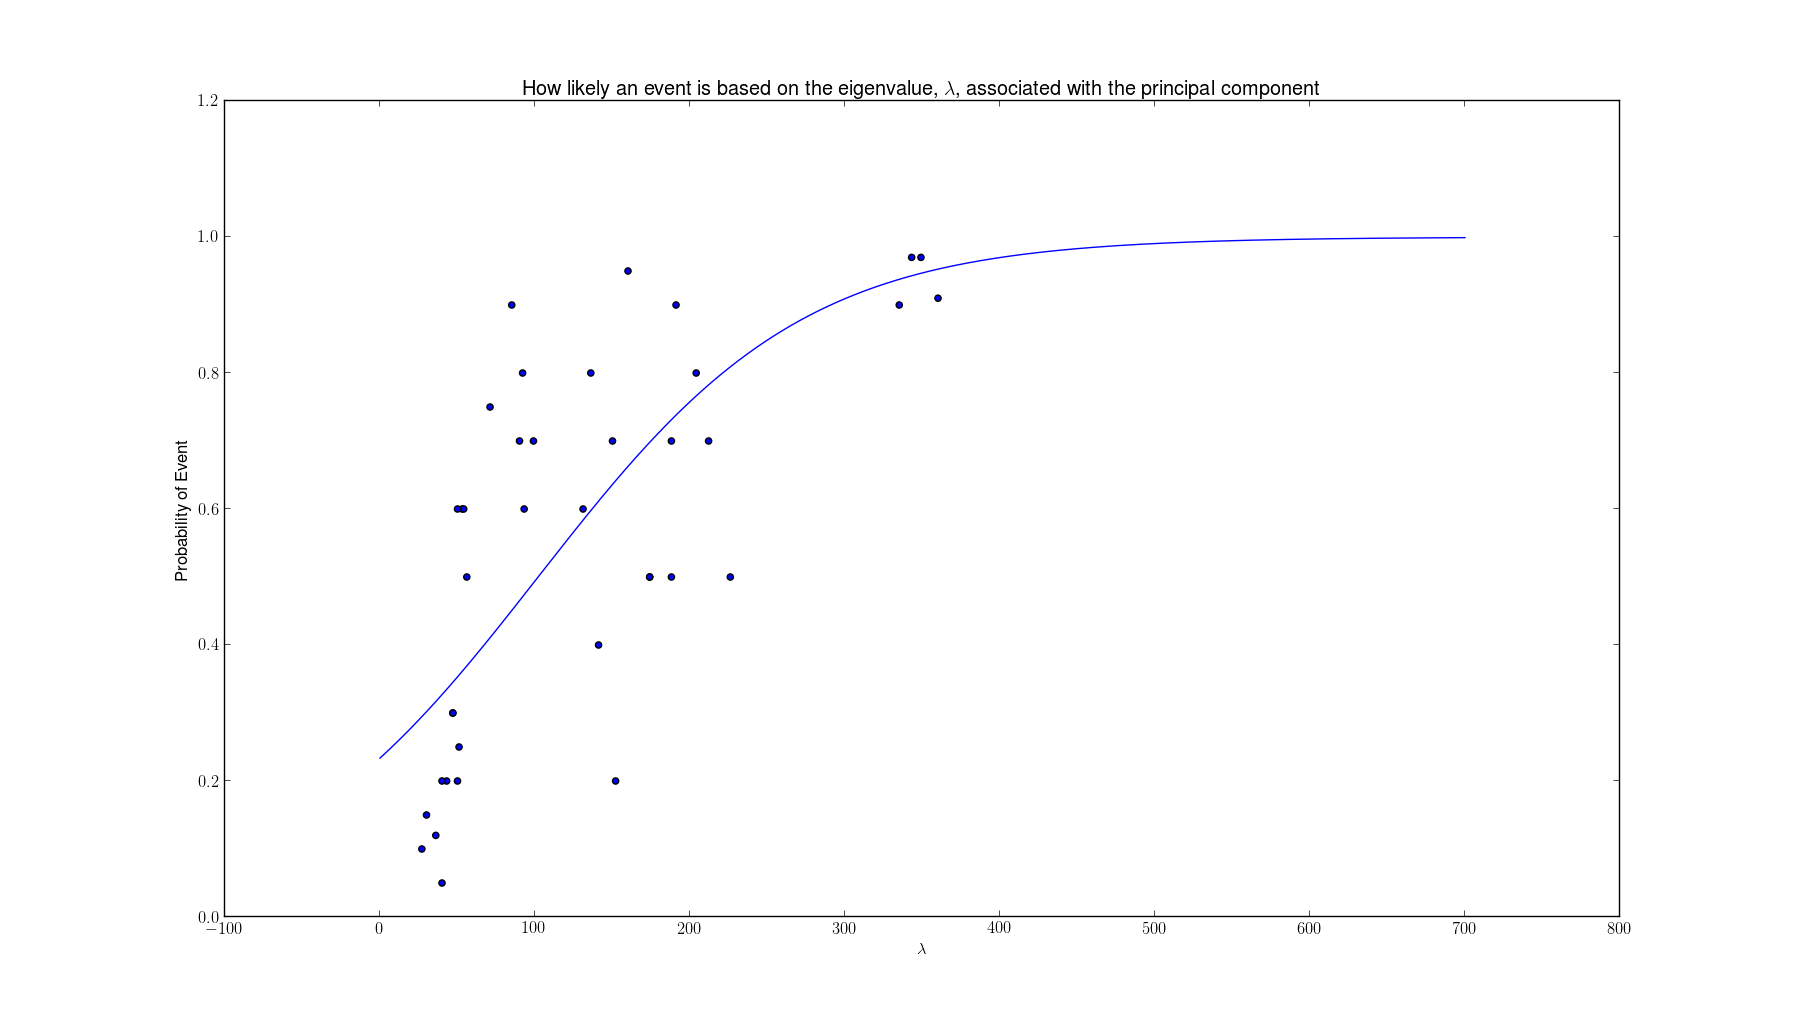
\includegraphics[scale=0.35]{Lambda_scatter.png}
\caption{An estimate of the mapping from the eigenvalue, $\lambda$, to the probability of an event. The range has been truncated to $\lambda \geq 0$ as $\lambda$ cannot take a negative value.}
\label{lambda_scatter}
\end{figure}

It should be noted that the labeling of the $\lambda_i$s is the only part of the procedure which is quite subjective, as it relies primarily on expert opinions, but like many probabilistic models, it is a necessary part to the process. 

Given that at this point in time only the $\lambda_i$ is used to indicate whether an event has taken place, this simple training scheme is sufficient, coupled with cross validation. However, in a further iteration, possibly more variables could be considered, in which case a more sophisticated predictor could be used, such as a Support Vector Machine. 

\subsubsection{How $\lambda$ Varies with the Window Size}
It is crucial to show how $\lambda$ is related to the window size in the application as this highlights the fact that the learned model of the previous section \ref{event_detection} is not universal to all problems, as the window size may change.

Mathematically, it is not hard to see the expected relationship. It is already known that if

\begin{equation*}
\smat = \left( \begin{matrix}
a_{1, 1} & a_{1, 2} & \cdots & a_{1, n} \\ 
a_{2, 1} & a_{2, 2} & \cdots &  a_{2, n} \\
\vdots & \vdots & \ddots & \vdots \\
a_{m, 1} & a_{m, 2} &\cdots &  a_{m, n} \\

\end{matrix} \right),
\end{equation*}
 then the co-occurence matrix used is given by:
\begin{equation*}
\covmat =
\left( \begin{matrix}
0 & \sum_{i=1}^m a_{i,1} a_{i,2} & \cdots & \sum_{i=1}^m a_{i,1} a_{i,n}\\ 
\sum_{i=1}^m a_{i,2} a_{i,1}  & 0& \cdots & \sum_{i=1}^m a_{i,2} a_{i,n}\\ 
\vdots & \vdots& \ddots & \vdots \\ 
\sum_{i=1}^m a_{i,n} a_{i,1} & \sum_{i=1}^m a_{i,n} a_{i,2} & \cdots & 0\\ 
\end{matrix} \right).
\end{equation*}

Therefore, the expected value of any entry in $\covmat$ can be given by

\begin{align*}
\mathbb{E}\{[\covmat]_{i, j}\} & =  \mathbb{E}\{\sum_{k=1}^m a_{k,i} a_{k,j}\},\\
& =  \sum_{k=1}^m \mathbb{E}\{ a_{k,i} a_{k,j}\},\\
& =  \sum_{k=1}^m \mathbb{E}\{ a_{k,i}\}\mathbb{E}\{ a_{k,j}\},\\
 & =   \sum_{k=1}^m p_1^2, \\
 & =   mp_1^2,
\end{align*}

if $i \neq j$ and 0 otherwise. This clearly shows that the larger $m$ is i.e. the number of rows of $\smat$, the higher the expected value of each of the off-diagonal elements of $\covmat$. This is why the expected $\lambda$ grows with $m$, the number of Tweets per window.

To demonstrate this further, an experiment is carried out to find the average $\lambda$ in the absence of an event, with different sizes of the data matrix $\smat$. This is done by creating $\smat$ and with a varied number of rows, and adding a 1 with some probability $p_1$ and a zero else, much like in section \ref{binary_data} for the first trial. This should simulate the scenario of the absence of an event since each entry will be independent and identically distributed, therefore so will each feature of each row. Then this matrix is run through the algorithm and the associated $\lambda$ is found. For each size of the matrix $\smat$ the process is repeated 10 times and an average $\lambda$ is obtained. This is then plotted, as in Figure \ref{lambda_vs_tweets}, and a first order polynomial has been fit through the points in the least squares sense. 
\begin{figure}[H]
\centering
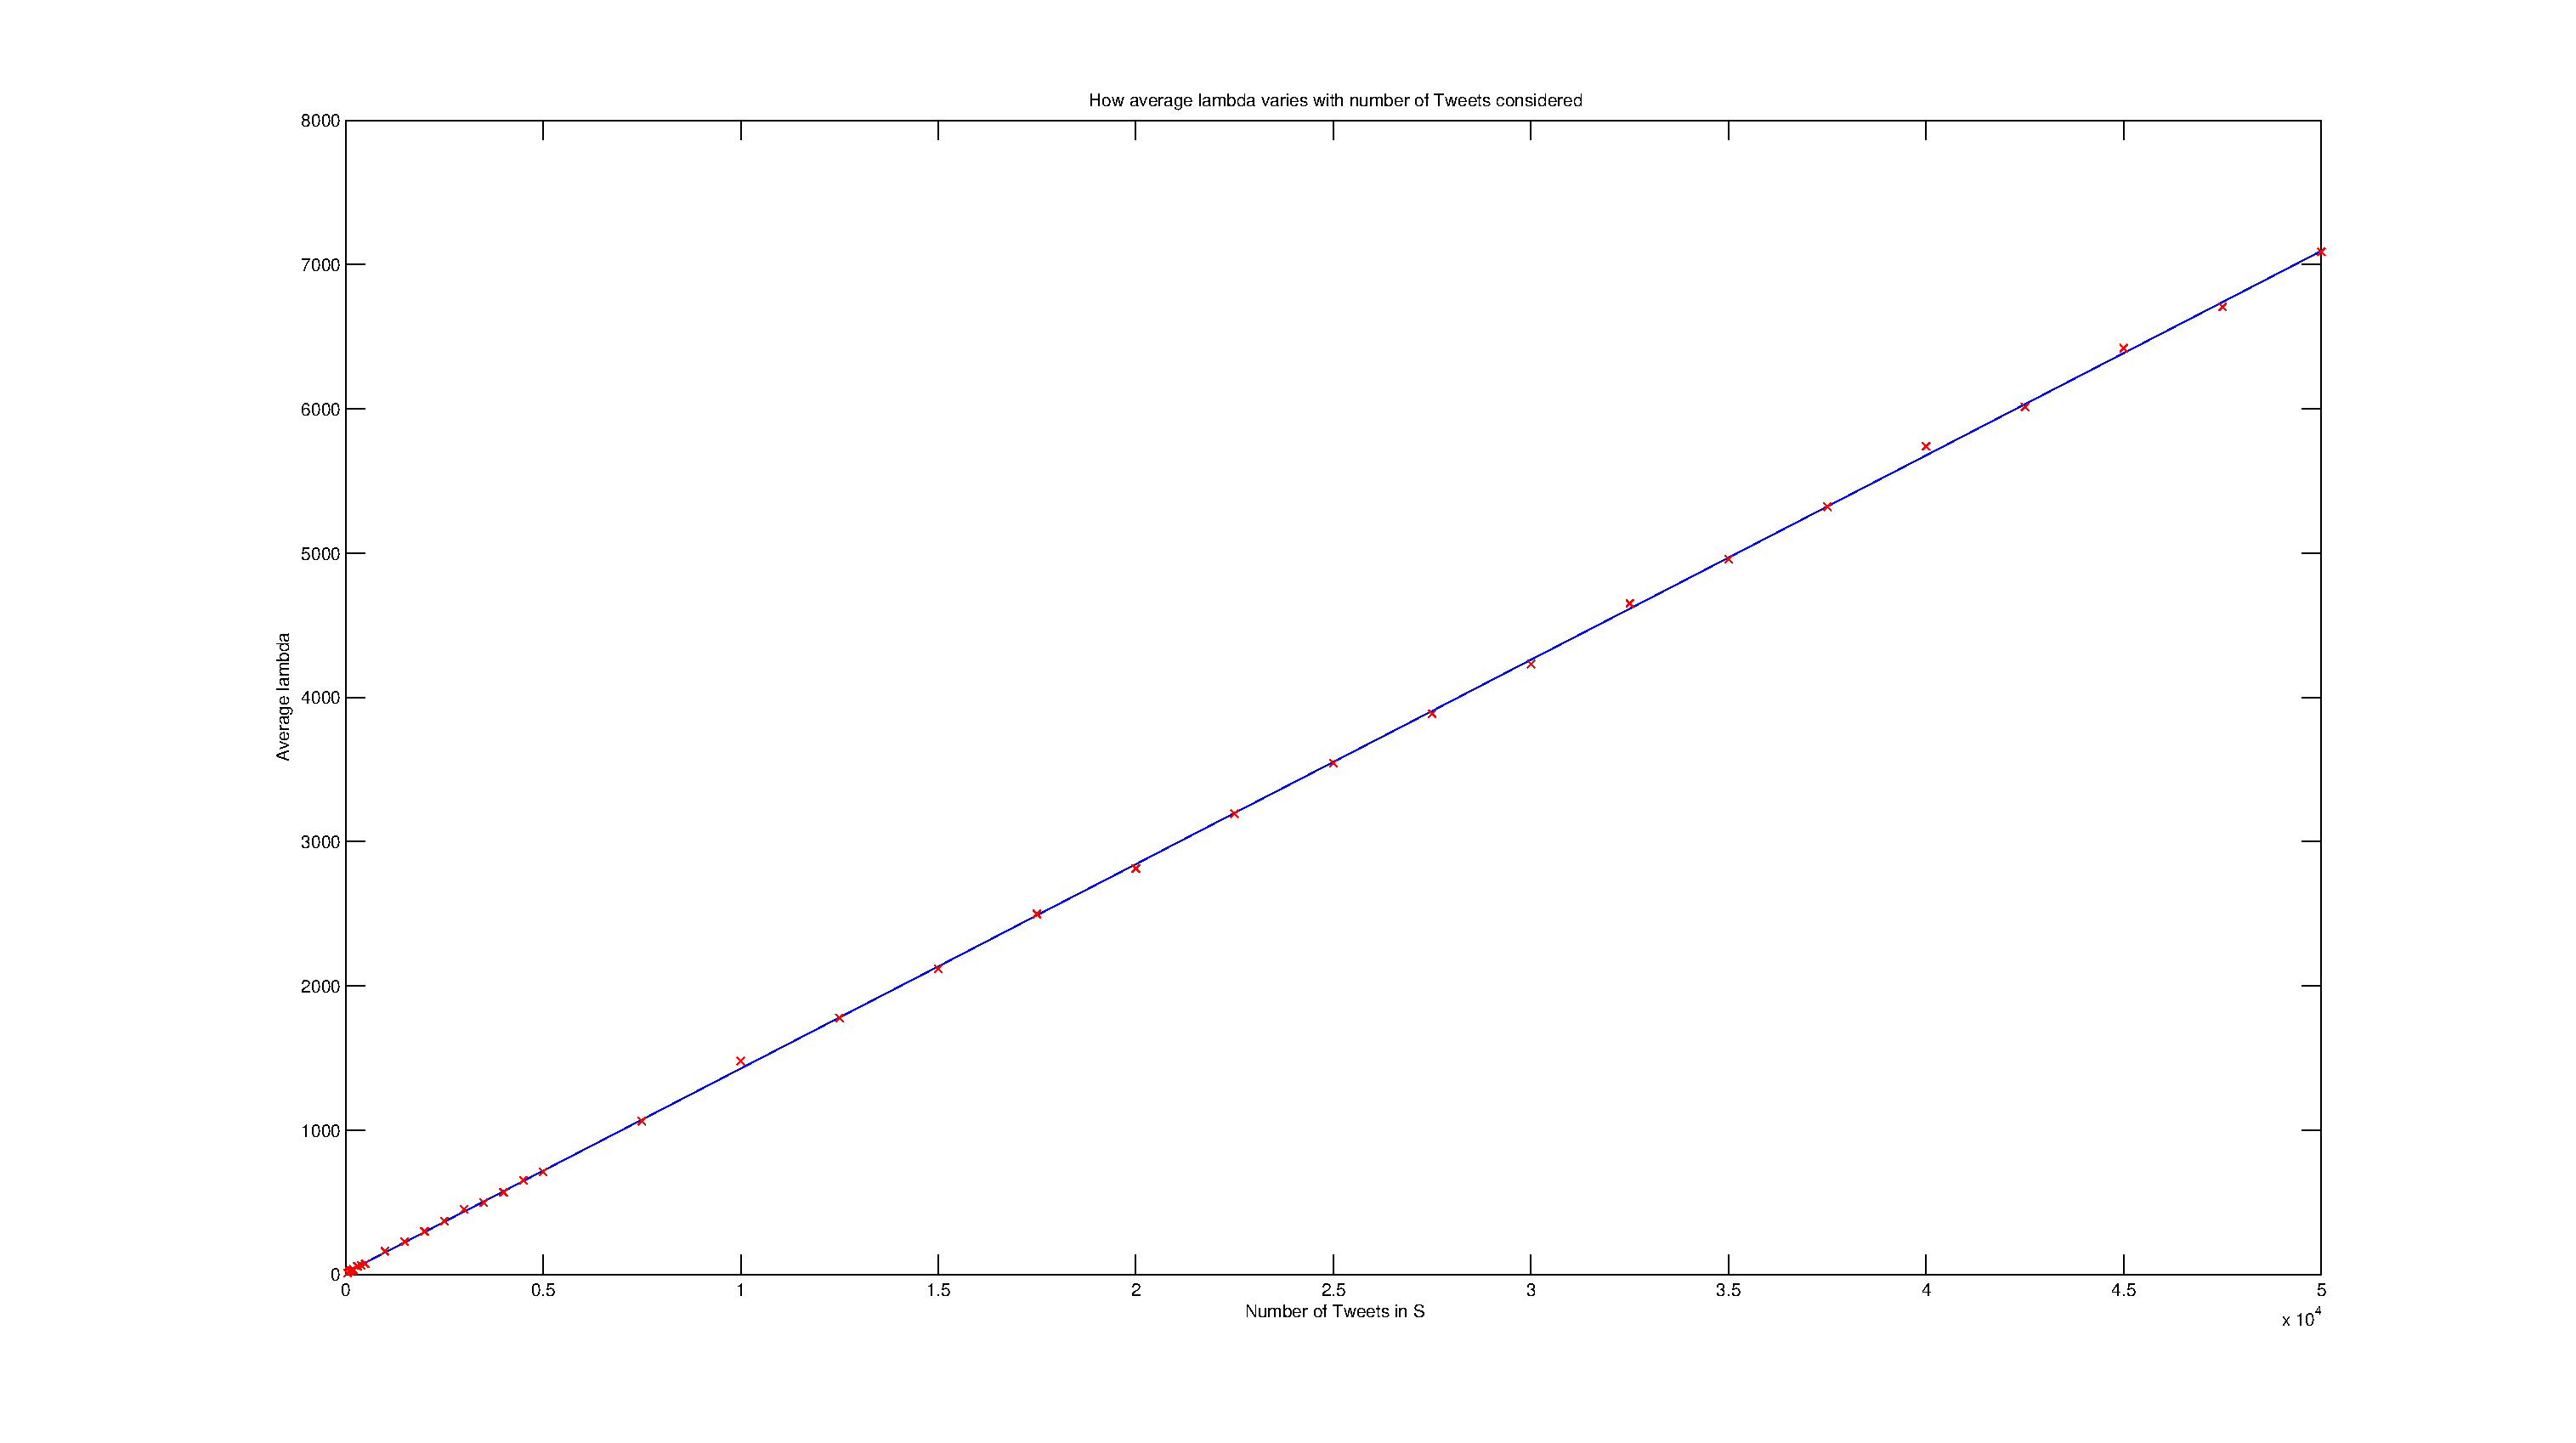
\includegraphics[scale=0.30]{lambda_vs_number_tweets.eps}
\caption{How the average $\lambda$ varies with the number of Tweets represented by the rows of $\mathbf{S}$.}
\label{lambda_vs_tweets}
\end{figure}

As is evident, the average $\lambda$ varies approximately linearly with the number of rows of $\smat$ in the absence of an event. This means that though the probability of an event with a window size of 5000 may be very likely for some certain $\lambda$, it would probably be very unlikely if a window size of 50000 were to be considered. This highlights the fact that a different model needs to be trained for each window size.

\subsection{Testing the Streaming Algorithm on London Data} 
\label{london_test}
After training the parameters to be able to find the events that are known and have been found previously and testing their predictive performance to ensure over-fitting hasn't taken place, the algorithm is run on the entirety of the data from London 2012 and the result can be seen in Figure \ref{testing_app_all_data}. 

In this case, soft classification is used as opposed to previously where a data point is either red to indicate an event or blue otherwise. This time a linear combination of red and blue is used to indicate the probability of an event taking place. To detect an event, one may attempt to take all points with a probability of greater than 0.6 possibly and look at the principal components.

\subsubsection{Results}
\begin{figure}[H]
\centering
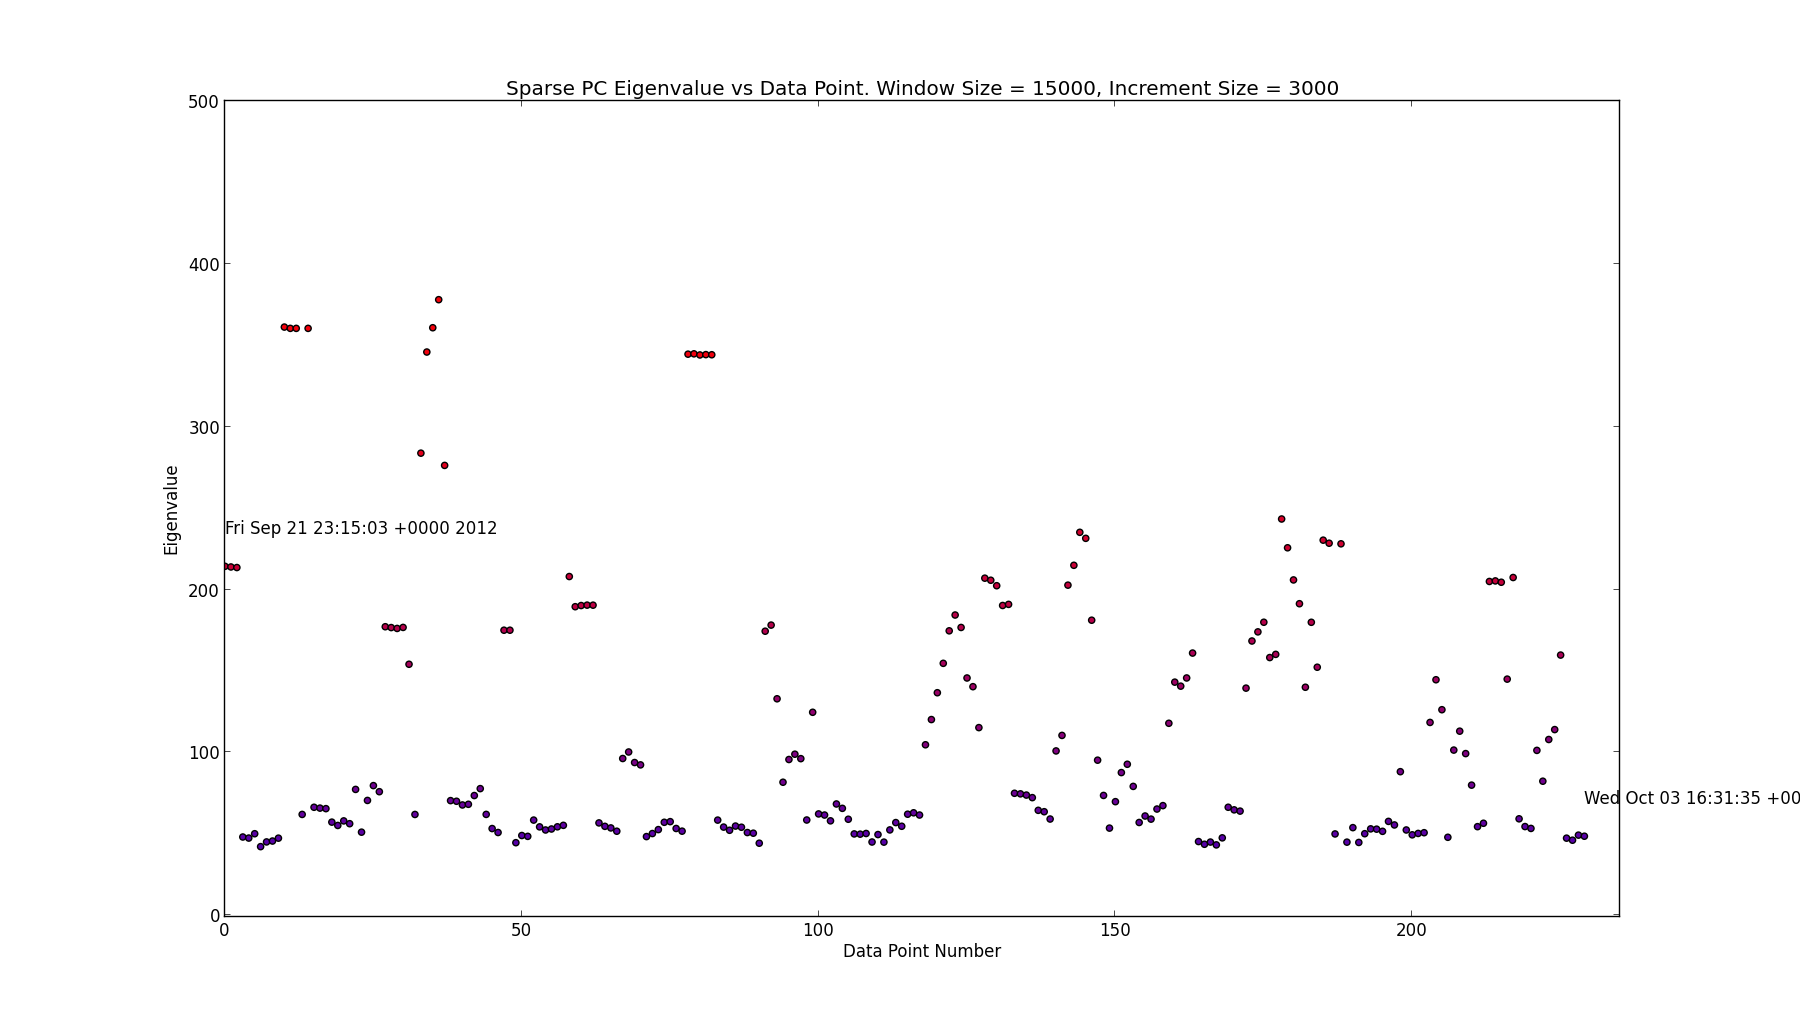
\includegraphics[scale=0.30]{Twitter_Data_All_Graph.png}
\caption{Testing the streaming application with a window size of 15000 Tweets and a shift of 3000 Tweets for each data point. Using the mapping from section \ref{event_detection} each point is now assigned a probability of being associated with an event, which is visualised as a linear combination of red and blue. The more red a point is, the more likely it is associated with an event. The start and end dates are labeled on the graph, as well as the start and end dates and times of an event. This corresponds to doing a calculation roughly every 1 hour 20 minutes.}
\label{testing_app_all_data}
\end{figure}

\begin{table}[H]

\begin{tabular}{| p{11cm}| r | l|}
\hline
Principal Component Words & $\lambda$ & Date\\
\hline
best, getting, please, could, ever, friends, retweet, sarah, married, matt & 212 & 21/09/2012	 \\
please, world, support, towards, flight, squad, homeless, morocco, donations, costs & 360 & 22/09/2012\\
terry, john, best, england, football, international, retired, news, retires, retirement & 359 &  23/09/2012\\
\st{thanks, only, hours, retweet, name, flight, cover, costs, deadline, rapper} & \st{190} & \st{24/09/2012}\\
please, follow, police, again, following, fallen, colleagues, recent, officers, murders & 343 & 26/09/2012\\
arsenal, emirates, game, giroud, stadium, coventry, city, gunners, blues, highbury & 140 & 26/09/2012\\
free, tomorrow, event, live, music, party, john, exhibitions, nightlife, clubbing & 136 & 28/09/2012\\
\st{night, late, early, till, driving, thursday, bird, lessons, tuesday, flexible}
& \st{202} & \st{28/09/2012}\\
night, free, event, live, tomorrow, music, club, borough, exhibitions, gigs & 98 & 29/09/2012\\
arsenal, chelsea, here, stadium, emirates, game, watch, gunners, blues, highbury & 202 & 29/09/2012\\
spurs, coys, great, game, united, done, first, half, trafford, thfc & 78 & 29/09/2012\\
\st{follow, please, tweet, babe, harry, forever, directioner, hola, pido, alma} & \st{134} & \st{30/09/2012}\\
tomorrow, free, live, music, club, event, comedy, borough, blues, lewisham & 77 & 30/09/2012\\
xfactor, through, rylan, year, over, nicole, should, louis, jake, shows & 164 & 30/09/2012\\
rydercup, europe, rydercup2012, golf, teameurope, great, rose, justin, goeurope, point & 192 & 30/09/2012\\
first, happy, october, month, birthday, \st{punch, pinch,} black, history, returns & 131 & 01/10/2012\\
happy, birthday, check, pics, blog, nathan, maxmonday, tickling, max's, exclusive & 226 & 01/10/2012\\
free, tomorrow, event, live, music, comedy, john, exhibitions, acoustic, sugarfoot & 94 & 01/10/2012\\
still, doing, next, again, year, week, marathon, huntingtons, adidas, teamsimran18 & 203 & 02/10/2012\\
\st{them, look, made, does, friends, name, cause, deserve, bought, lwwy} & \st{142} & \st{02/10/2012}\\

\hline
\end{tabular}
\caption{Some of the principal components sampled after running the algorithm on all the data from London 2012. The samples taken have a $\lambda > 70$ and it has been rounded to the nearest unit. The dates are also given. Words and dates that are crossed out indicate that they are not relevant for an event.}
\label{streaming_test}
\end{table}

Table \ref{streaming_test} shows some of the results sampled after running the algorithm on the all the data. There are a few things to note. Firstly, in this test run it can be seen that any principal component with a $\lambda > 300$ is almost certainly linked to an event (in this case it definitely is), which agrees with the logistic function derived in \ref{event_detection}. Furthermore, no event has been found with a $\lambda < 70$, again agreeing with the logistic function derived in \ref{event_detection}. 

Added to this, it is interesting to see that not only have all the principal components previously discovered, in section \ref{first_three_pcs}, been found but that more have also emerged, which is due to the calibration of the window size, which has been significantly reduced and has also been transformed into with a sliding window. For example, the second row of the table is related to a Twitter campaign which aimed at raising funds for the Homeless Football World Cup team for Morocco. This was previously in the same window as the news for John Terry's retirement and was overpowered by it.

\subsection{Testing the Streaming Algorithm on Different Data}
As previously mentioned, to measure the general effectiveness of the algorithm, it must at least be tested on other Twitter data also from a different geographical location. Therefore, using the Twitter API \footnote{https://dev.twitter.com/docs/api/streaming, Accessed: 28-05-2014}, more data has been collected from the United States of America, the coordinates, given as a bounding box of (latitude, longitude) coordinates with the SW corner given first and then the NE, are (-126.8,33.2),(-76.7,48.8).\footnote{Found using the online tool http://boundingbox.klokantech.com/.} A modest amount of data has been collected, namely from 7:21 a.m. on the 28th May 2014 to 10:49 a.m. on the 28th May 2014, which is roughly 3.5 hours of data, which amounts to about 76000 Tweets. Just as a measure of comparison, it can be seen that in just 3.5 hours in the U.S.A. there has been more Tweets that in a day in London, which is not surprising, but gives rise to interesting results. 

\begin{figure}[H]
\centering
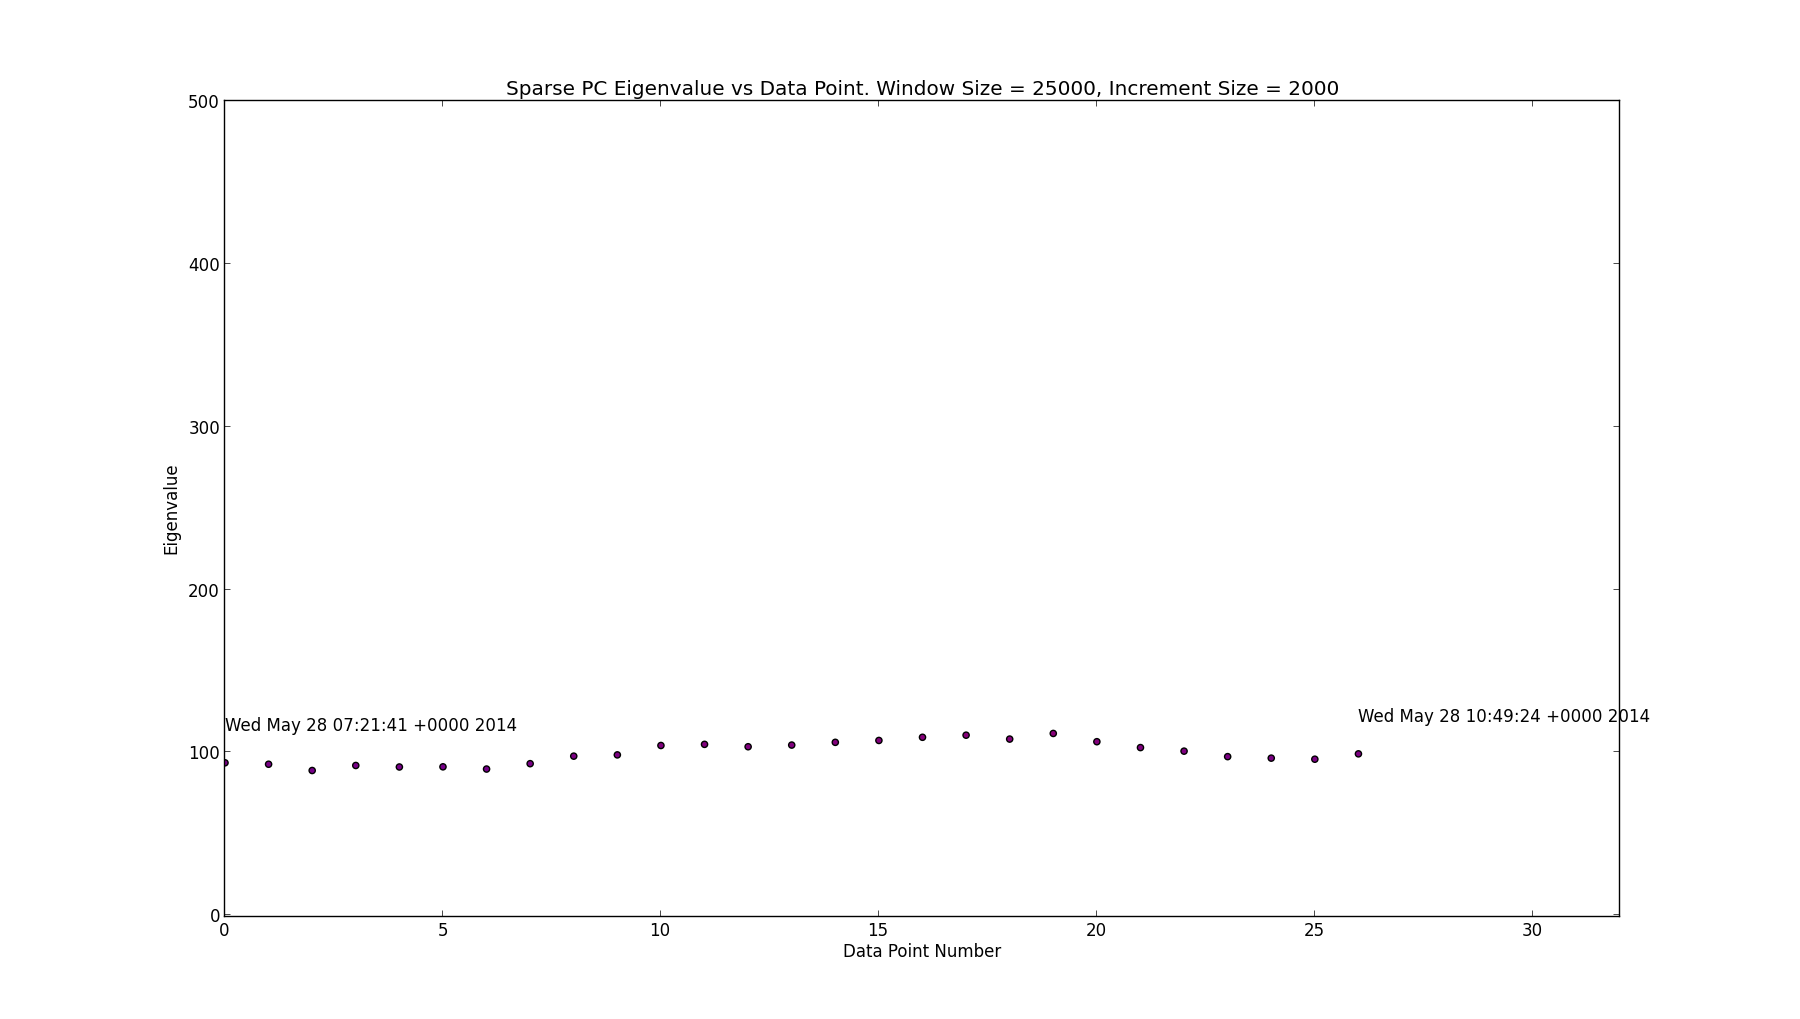
\includegraphics[scale=0.25]{Testing_Streaming_App_25000_2000_USA.png}
\caption{Testing the streaming application on the U.S.A data with a window size of 25000 Tweets and a shift of 2000 Tweets for each data point. Using the mapping from section \ref{event_detection} each point is now assigned a probability of being associated with an event, which is visualised as a linear combination of red and blue. The more red a point is, the more likely it is associated with an event. The start and end dates are labeled on the graph, as well as the start and end dates and times of an event. This corresponds to doing a calculation for a window size of roughly 7 minutes.}
\label{testing_app_25000_usa}
\end{figure}

\begin{figure}[H]
\centering
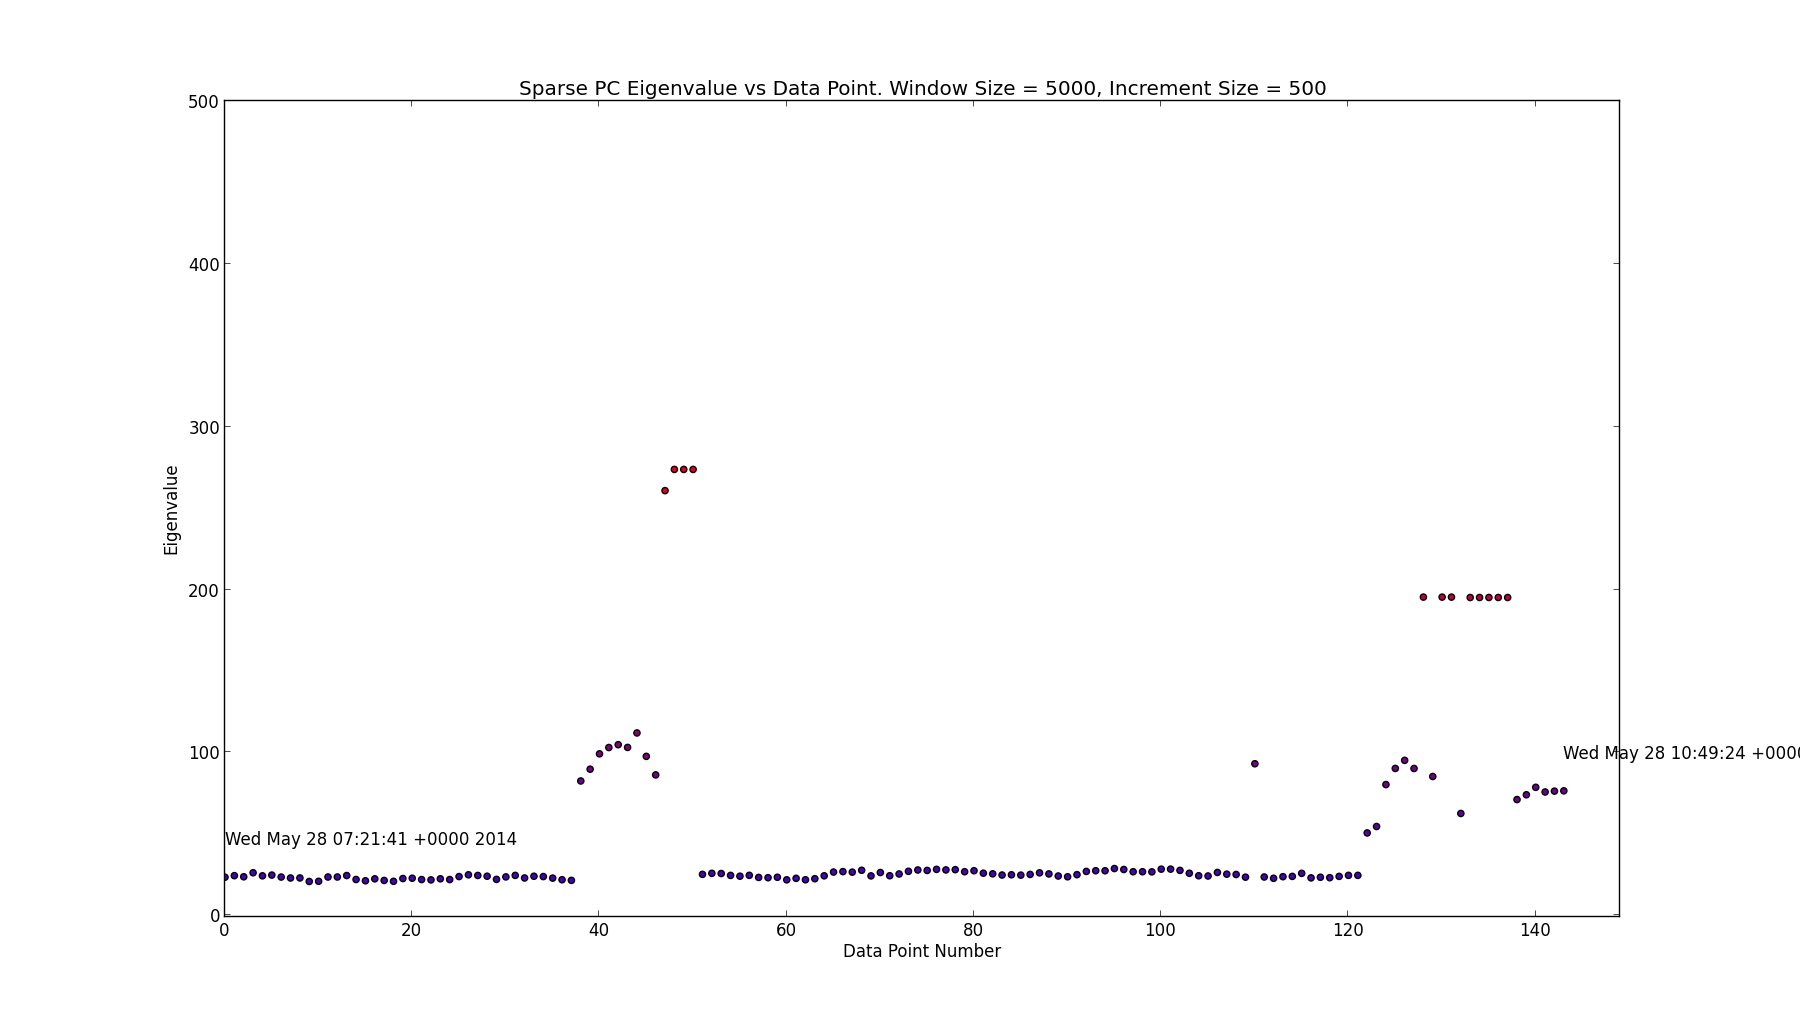
\includegraphics[scale=0.25]{Testing_Streaming_App_5000_500_USA.png}
\caption{Testing the streaming application on the U.S.A data with a window size of 5000 Tweets and a shift of 500 Tweets for each data point. Using the mapping from section \ref{event_detection} each point is now assigned a probability of being associated with an event, which is visualised as a linear combination of red and blue. The more red a point is, the more likely it is associated with an event. The start and end dates are labeled on the graph, as well as the start and end dates and times of an event. This corresponds to doing a calculation for a window size of roughly 1 and 1/2 minutes.}
\label{testing_app_5000_usa}
\end{figure}

From Figures \ref{testing_app_25000_usa} and \ref{testing_app_5000_usa}, it can be seen that, once again, different values for the window size and for the increment size lead to different results. 

In the first case, all points are pretty unlikely to be associated with an event. In the second case, however, it can be seen that there are two distinct peaks in the value of $\lambda$. These are both associated with the same event and the words that appear as the supports can be found in Table \ref{streaming_test_us}. They refer to a flash flood being issued in Charleston and Jackson on the day which woke many people up and there was a surge of Tweets complaining about it. It should be noted that each window is compromised by roughly 7 minutes of date in the second scenario which is quite different to the case explored in section \ref{london_test} where each window has about 2.5 hours of Twitter data, which again shows how important different parameters are for different window sizes. 
\begin{table}[H]
\center
\begin{tabular}{| p{11cm}| r | l|}
\hline
Principal Component Words & $\lambda$ & Date\\
\hline
\st{watch}, \st{wanna}, until, issued, flood, flash, \st{someone}, charleston, jackson, \st{netflix} & 274 & 28/05/2014	 \\
want, until, watch, days, flash, flood, issued, \st{college}, \st{state}, \st{mobile}& 195 & 28/05/2014	 \\
\hline
\end{tabular}
\caption{The principal components found after running the algorithm on the data from the U.S.A. The samples taken have a $\lambda > 70$ and it has been rounded to the nearest unit. The dates are also given. Words and dates that are crossed out indicate that they are not relevant for an event.}
\label{streaming_test_us}
\end{table}

%TODO Show that the parameters in this case are not optimal and show that there are differences in the scale of the data
%TODO Show why larger number of tweets considered gives rise to a larger average eigenvalue. demo_scale_S_eigenvalue in Matlab.
\subsection{Calculating Multiple Principal Components Per Iteration}
%TODO Don't know if this will add any value
\subsection{Increasing the Performance of the Algorithm}
%TODO
\begin{comment}
- Use the streaming algorithm with the threshold detection vs the streaming without it and show that the time it takes for the threshold is less and for not a significant deterioration in the pcs found. Try this.
\end{comment} 
\subsubsection{Building the Co-occurrence Matrix $\covmat$}
One method to increase the speed of the algorithm, and therefore the rate at which it can operate, is by taking note that, if the increment size is fairly small compared to the size of the window, then lots of unnecessary calculation is being done by actually building the co-occurrence matrix upon each iteration. 

This can be shown by looking at two consecutive windows, given in the matrix form: 
\begin{equation*}
\smat = \left(\begin{matrix}
\smat_{\text{old}}\\
\smat_{\text{common}}\\
\smat_{\text{new}}
\end{matrix}\right),
\end{equation*}
where the first window is $\left(\begin{matrix}
\smat_{\text{old}}^T&
\smat_{\text{common}}^T\\
\end{matrix}\right)^T
$ and the second is $\left(\begin{matrix}
\smat_{\text{common}}^T&
\smat_{\text{new}}^T\\
\end{matrix}\right)^T
$
and each $\smat_{\text{old}}, \smat_{\text{new}} \in \mathbb{Z}^{k \times n}$, where $k$ is the increment size, in number of Tweets, and $\smat_{\text{common}} \in \mathbb{Z}^{(m-k) \times n}$ where $m$ is the window size. 

Let $\covmat_{\text{old}}$ be the old non-hollow co-occurrence matrix and $\covmat_{\text{new}}$ be the new one. Then it can be seen that

\begin{align*}
\covmat\old & = \left( \begin{matrix}
\smat\old^T & \smat\common^T
\end{matrix}\right)\left( \begin{matrix}
\smat\old \\ \smat\common
\end{matrix}\right),\\
& = 
\smat\old^T \smat\old+ \smat\common^T \smat\common,
\end{align*}
 and similarly, 
\begin{align*}
\covmat\new & = \left( \begin{matrix}
\smat\common^T & \smat\new^T
\end{matrix}\right)\left( \begin{matrix}
\smat\common \\ \smat\new
\end{matrix}\right),\\
& = 
\smat\common^T \smat\common+ \smat\new^T \smat\new,
\end{align*} 
therefore, 
\begin{equation}
\covmat\new = \covmat\old - \smat\old^T \smat\old + \smat\new^T\smat\new.
\end{equation}

This means that upon each iteration instead of calculating the whole matrix again, which takes $O(mn^2)$, two matrices with much less elements must be considered, bringing the calculation of the co-occurrence matrix to $O(kn^2)$ where $k << m$. For instance, for the parameters chosen above for the London Twitter data, $m = 10000$ and $k = 1000$, therefore, on average a computational saving of about $80\%$ is saved (due to there being two matrices that need to be calculated, not just one). Since populating the matrix $\smat$ is the actual bottleneck in the whole streaming algorithm this would give rise to a great performance increase. 

In this scenario the change in the Bag-of-Words is not considered for simplicity, but with some alterations, this can be adapted to work for the more general case.


\subsection{Limitations}
%TODO
\begin{comment}
- Explain how taking a different geographical location would require the whole procedure to be redone with the logistic function re-calibrated and the window size and increment also. 
\end{comment}
Something to note is that for $\lambda \in (70, 300) $ there is a lot of uncertainty about whether a principal component indicates an event. On the one hand words can be used quite often together and therefore can result in a principal component, if there are no popular events during the same period, for instance the fourth row of Table \ref{streaming_test}. On the other hand however, some principal components are clearly consistent with events, however, they may not be that popular. An example of this can be seen by looking at the 11th row of the table which is related to a game of football in which Tottenham beat Manchester United at the Old Trafford on that day. Not having taken place in London may have also contributed to the fact that it was not that popular, but it can be seen that, though the associated $\lambda$ is quite low, it definitely is related to a genuine event. 

This uncertainty makes it difficult to assign hard classification thresholds and this is why a probabilistic approach is instead considered. What can be said though, is that if there is an event of significant popularity in the area considered, the algorithm will return words related to this.

Moreover, given a larger geographical area, the whole procedure i.e. training of the parameters, must be redone, which takes time. 


\clearpage
\section{Conclusion}
%TODO
\section{Further Work}
%TODO
\begin{comment}
- Put in Appendix a section on how SVM works.
- Explain how tracking can be done by taking the inner product of the vectors and seeing how close to 1 they come. 
\end{comment}
As with most areas of research, there is room for improvement but given the time constraints and the lack of data some of these areas must be left for a later time. 

\subsection{Clustering of features in the Bag of Words}
Firstly, in many of the principal component examples words appear that are from the same root or are similar in meaning, for instance, in the John Terry example, the words ``retire'', ``retired'' and ``retirement'' all appear in the same principal component. The problem with this is that since they are considered as separate features, even though they actually aren't, the appearance of one of these words may be distributed in a population of Tweets across all three of them, therefore decreasing the total count of the feature. This means that for some events, where many similes may be used, these may not be found purely because the words have not been aggregated together and thus the Sparse PCA algorithm has not kept them. Having a more sophisticated parser in the pre-processing step which could do this would ensure much better results and would be much more robust to vocabulary or spelling differences.

\subsection{Generalising the Parameter Selection}
Furthermore, as mentioned previously, the parameters have been trained in this instance to work on Tweets that have been collected from the area of London at a specific time, but would not work optimally for a location of a different size or with a different density of Twitter users. Therefore, a lot more research could go into finding a method of estimating these parameters, either in an adaptive fashion or by pre-computing some of the parameters and using a lookup table.

\subsection{Improving the Event Detection Parameter}
\subsubsection{Using Previous $\lambda$ Values}
Using more parameters to identify whether an event has happened should also be considered. For instance, taking into account previous values of $\lambda$ would also be very beneficial. Equation \eqref{logit} could take the more general form

\begin{equation}
p(\lambda_i)= \frac{1}{\left( 1 + e^{-\mathbf{w}^T\bm{\lambda}}\right)},
\label{logit_general}
\end{equation}
where $\bm{\lambda}$ takes the form $\left(\begin{matrix}
1 & \lambda_i & \lambda_{i-1} & \cdots & \lambda_{i-n}
\end{matrix}\right)^T$ where $n+1$ is the number of previous $\lambda$ values to consider. 

\subsubsection{Using a More Sophisticated Classifier}
Alternatively, a more sophisticated method could be considered, for example, using a Support Vector Machine. For this to work many more labeled training examples would need to be considered. Here roughly 12 days of data has been used and has given rise to about 16 significant events. This means that only 16 data points can be used as positive targets to train the classifier. Given more time, much more data could be collected, for instance, over the period of possibly 2 months. This data could then actually be manually classified and then a Support Vector Machine could be trained using a proportion of this data. This could then be validated using the other portion, which is a commonly used method in Machine Learning to test whether a model has not been fit too well to the data such that it cannot generalise to new data points.

\subsubsection{Using the Rate of Tweets}
The rate of Tweets could also be considered, as in \cite{eventtwitter}. 
For example, the same linear classifier could be used plus an additional term to give
\begin{equation*}
\mathbf{w}_t^T \mathbf{T} + \mathbf{w}_r^T \mathbf{R} + \mathbf{w}_\lambda^T \mathbf{\Lambda} \geq A,
\end{equation*}
where $\mathbf{T} \in \mathbb{R}^5$ is a vector of the Tweet rate for 5 consecutive time steps, with the middle one being the current, $\mathbf{R} \in \mathbb{R}^5$ is the same but for the Retweet rate and $\mathbf{\Lambda} \in \mathbb{R}^5$ is for the eigenvalues returned by the algorithm. $\mathbf{w}_i$ are the weights for each feature, trained for the classifier and $A$ is the threshold, also trained.
In this case, the window size could be determined by a time period rather than a number of Tweets.

\subsubsection{Using Other Parameters Provided by Twitter}
Something else that could be used for classification purposes could be the geocode parameter which indicates where the Tweet has come from geographically. The reasoning behind this is simple. For instance, some events may be quite specific to some borough of London, e.g. a concert of some sort in the Royal Albert Hall, and therefore, there is a possibility that a lot of the Tweets will come from areas around the Royal Albert Hall and therefore, these would be a lot more probable to be associated with events. 

Other parameters included in the JSON returned by the Streaming API of Twitter could also be used as features. 

\subsubsection{Tracking Events}
%TODO Check this
Another useful feature for the application would be to be able to track whether a previous event is the same as a current event, if they are consecutive. For instance, it may be that two events are taking place, one after the other, and it just so happens that the algorithm returns very similar eigenvalues for both. Given the time series alone, one may infer that just one long event has taken place, however, looking at the words associated with the principal components, it would be evident that they would be very different. In this case, an automatic way of detecting this would be to take the dot product between the two principal components and check whether the result would be close to 1. If this were to be the case, the two events would be classified as equal, else they would be classified as different. 
\clearpage

\bibliography{bibliography}
\bibliographystyle{plain}
\clearpage

\section{Appendix}\label{appendixa}

\appendix
\pagenumbering{Roman}

\section{PCA Formulation Explained (A variant of \cite{bishop})}

Consider a set of observations $\{\mathbf{x}_n\}$ for $n = 1, ..., N$ and each $\mathbf{x}_n \in \mathbb{R}^D$, to project the data onto just one dimension whilst keeping the maximum amount of variation possible (and therefore information), we can project the data onto one D-dimensional vector, $\mathbf{u}_1 \in \mathbb{R}^D$. The mean of the projected data is then $\mathbf{u}_1^T \mathbf{\overline{x}}$, where
\begin{equation*}
\mathbf{\overline{x}} = \frac{1}{N} \sum_{n = 1}^N \mathbf{x}_n 
\end{equation*} 
the sample mean of the observed data.

The sample variance of the projected data can then be given by
\begin{equation*}
\frac{1}{N} \sum_{n = 1}^N \{\mathbf{u}_1^T\mathbf{x}_n -  \mathbf{u}_1^T\mathbf{\overline{x}}_n\}^2
\end{equation*} 
\begin{equation*}
\mathbf{u}_1^T \left( \frac{1}{N} \sum_{n = 1}^N \left(\mathbf{x}_n - \mathbf{\overline{x}}_n\right)\left(\mathbf{x}_n - \mathbf{\overline{x}}_n\right)^T \right) \mathbf{u}_1
\end{equation*} 

Taking notice that 
\begin{equation*}
\frac{1}{N} \sum_{n = 1}^N \left(\mathbf{x}_n - \mathbf{\overline{x}}_n\right)\left(\mathbf{x}_n - \mathbf{\overline{x}}_n\right)^T 
\end{equation*} 
is just the covariance matrix of the data, call it $\mathbf{S}$, we can the say that:
\begin{equation}
\mathbf{u}_1^T \mathbf{S} \mathbf{u}_1
\label{uSu}
\end{equation} 

Therefore, if we would like to maximise the variance of the projected data, we need to maximise \eqref{uSu}. This can obviously be maximised by letting $\|\mathbf{u}_1\| \to \infty$, without taking into account the actual direction of $\mathbf{u}_1$, however this is not what is desired. What is actually needed is the direction in which the data varies most and not the actual length of the vector itself. A constraint is therefore imposed such that $\|\mathbf{u}_1\| = 1$ and then a Lagrange multiplier is introduced, $\lambda_1$. The resulting equation is as such:


\begin{equation*}
\mathbf{u}_1^T \mathbf{S} \mathbf{u}_1 - \lambda_1 (1 - \mathbf{u}_1^T \mathbf{u_1})
\label{lagrange_uSu}
\end{equation*} 

Which by setting the derivative with respect to $\mathbf{u}_1$ to zero, the following is attained:


\begin{equation*}
\mathbf{S} \mathbf{u}_1 = \lambda_1  \mathbf{u_1}
\label{eig_uSu}
\end{equation*} 

Which means that $\mathbf{u}_1$ is maximised by finding the eigenvector with the largest eigenvalue $\lambda_1$. Similarly to find the $M$ principal components, the eigenvectors of the covariance matrix with the $M$ highest eigenvalues must be calculated.
\clearpage
\section*{B. Useful Intuition for the Co-occurrence Matrix $\mathbf{A}$}
Consider a matrix, $S\in \mathbb{R}^{m\times n}$, where $m$ is the number of Tweets and $n$ is the number of features that the tweets are evaluated on, in this case the Bag-of-Words. Performing $S^TS = A$ where $A \in \mathbb{R}^{n\times n}$. 

By example, imagine:

\begin{equation}
\smat = \left( \begin{matrix}
a_{1, 1} & a_{1, 2} & a_{1, 3} \\ 
a_{2, 1} & a_{2, 2} & a_{2, 3} \\
a_{3, 1} & a_{3, 2} & a_{3, 3} \\
a_{4, 1} & a_{4, 2} & a_{4, 3} 
\end{matrix} \right)
\end{equation}

\begin{equation}
\covmat = \smat^T\smat =
 \left( \begin{matrix}
a_{1, 1} & a_{2, 1} & a_{3, 1} & a_{4, 1} \\ 
a_{1, 2} & a_{2, 2} & a_{3, 2} & a_{4, 2} \\ 
a_{1, 3} & a_{2, 3} & a_{3, 3} & a_{4, 3} \\ 

\end{matrix} \right)
\cdot \left( \begin{matrix}
a_{1, 1} & a_{1, 2} & a_{1, 3} \\ 
a_{2, 1} & a_{2, 2} & a_{2, 3} \\
a_{3, 1} & a_{3, 2} & a_{3, 3} \\
a_{4, 1} & a_{4, 2} & a_{4, 3} 
\end{matrix} \right)
\end{equation}


\begin{equation}
\covmat =
\left( \begin{matrix}
\sum_{i=1}^4 a_{i,1}^2& \sum_{i=1}^4 a_{i,1} a_{i,2} &  \sum_{i=1}^4 a_{i,1} a_{i,3} \\ 
\sum_{i=1}^4 a_{i,2}a_{i, 1} & \sum_{i=1}^4 a_{i,2}^2 &  \sum_{i=1}^4 a_{i,2} a_{i,3} \\ 
\sum_{i=1}^4 a_{i,3}^2& \sum_{i=1}^4 a_{i,3} a_{i,2} &  \sum_{i=1}^4  a_{i,3}^2 \\ 
\end{matrix} \right)
\end{equation}

Since $a_{i, j} = 1$ when the word $j$ appears in Tweet $i$ and otherwise 0, the resulting matrix is basically a symmetric matrix with entry $(i, j)$ being composed of the number of times word $j$ occurs with word $i$ in the same Tweet over all the Tweets. The diagonal is  therefore the number of times the word $j$ appears over all the Tweets.

This is basically a form of clustering i.e. words that occur frequently together will have high corresponding values in the matrix $\covmat$ and can be seen as a weighted adjacency matrix.

\section{Laplacian Matrix}
Let a graph be defined as $G = (V, E, w)$ where $V$ is the set of vertices and $E$ is the set of edges, which are given as tuples of elements in the set $V$ and $w: E \rightarrow \mathbb{R}^+$ gives the weight associated with each edge. 

The adjacency matrix of this graph is given by

\begin{equation*}
[\mathbf{A}]_{i, j} = \begin{cases}
w(i, j), & \text{if}\ (i, j) \in E \\
      0, & \text{otherwise}
\end{cases}, 
\end{equation*}
i.e. the $(i, j)$th entry is given by the weight of the edge connecting the  vertex $i$ to vertex $j$.
The degree matrix is then given by

\begin{equation*}
[\mathbf{D}]_{i, i} = 
\sum_j [\mathbf{A}]_{i, j},
\end{equation*}
which is given by the sum of all the weights of the edges coming out of vertex $i$.

The Laplacian, $\mathbf{L}$ is then given by
\begin{equation*}
\mathbf{L} = \mathbf{D} - \mathbf{A}.
\end{equation*}

For an unweighted graph, each edge is taken to have weight 1.

The Laplacian matrix has many useful properties for graph theory.
\section{Support Vector Machine}
\section{Code}
All code written for this project can be found on Github and can be cloned by using the clone https:
\url{https://github.com/theopavlakou/projectapplication.git}


\section{User Guide}
%TODO is this necessary 

\section{Resources}
%TODO Here mention the laptop used and the APIs
\end{document}
